%%%%%%%%%%%%%   DEFINITIONEN   %%%%%%%%%%%%%%%
%\pdfminorversion=5 
\RequirePackage[2020-02-02]{latexrelease}
\documentclass[12pt,a4paper,oneside]{book}

%Packages
\usepackage[utf8]{inputenc}
\usepackage[USenglish]{babel}
\usepackage[T1]{fontenc}
\usepackage{amsmath}
\usepackage{amsfonts}
\usepackage{amssymb}
\usepackage{mathrsfs}
\usepackage{bbold}
\usepackage{xfrac}
\usepackage{graphicx}
\usepackage{xcolor}
\usepackage[textwidth=150mm,bottom=25mm,top=25mm,headsep=5mm,bindingoffset=5mm]{geometry}
\usepackage{listings}
\usepackage{fancybox}

\usepackage[small,bf]{caption} %Schönere Beschriftungen für Abbildungen und Tabellen
\captionsetup{width=1\textwidth,skip=5pt,format=plain,indention=5pt}
\usepackage{sidecap}
\sidecaptionvpos{figure}{t}
\usepackage{subcaption} %subfigures
\usepackage{booktabs} %Schönere Tabellen
\usepackage{fancyhdr} %Schönere Kopfzeile
%\usepackage[section]{placeins} %Abbildungen und Tabellen bleiben in ihrer Section
\usepackage{blindtext} %Einfügen von Blindtext über \blindtext
\usepackage{siunitx} %Einstellungen für Dezimaltrennzeichen und Definitionen in siunitx.cfg
\usepackage[autostyle=true,german=quotes]{csquotes} %Verwendung von Anführungszeichen über \enquote{Text}
\usepackage[toc,page]{appendix} %um eine Titelseite "Anhang" vor dem eigentlichen Anhang einfügen zu können

%Druckt den Hinweis "Entwurf" mit Datum auf jede Seite. Zum deaktivieren printwatermark=false setzen
\usepackage[printwatermark=true]{xwatermark}
\newwatermark[allpages,textcolor=gray!70,angle=0,xpos=68,ypos=-135,fontsize=14pt,fontfamily=phv]{Entwurf\ -\ \the\day.\the\month.\the\year}

%multirow in tabellen
\usepackage{multirow}

%%prüfe nach nicht verwendeten bib einträgen
%\usepackage{refcheck}

\usepackage{tocvsec2}
\settocdepth{subsection}


%Appendices -> Anhang
%\renewcommand*\appendixpagename{Anhang}
%\renewcommand*\appendixtocname{Anhang}

%neue Pakete
\usepackage{verbatim} %kommentare
\usepackage[numbers,comma,sort&compress]{natbib} %bibliographie
\usepackage{commath}
\usepackage{mathtools}
\usepackage[figuresleft]{rotating} %seite quer
\usepackage[nohyperlinks]{acronym} %abkürzungsverzeichnis
%vor chapter weniger platz
%\usepackage{etoolbox}% http://ctan.org/pkg/etoolbox
%\makeatletter
%\patchcmd{\@makechapterhead}{\vspace*{50\p@}}{}{}{}% Removes space above \chapter head
%%\patchcmd{\@makeschapterhead}{\vspace*{50\p@}}{}{}{}% Removes space above \chapter* head
%\makeatother


%algorithmcx
\usepackage{algorithm}
\usepackage{algpseudocode}

%abstände
\usepackage{titlesec}
\titlespacing\section{0pt}{12pt plus 4pt minus 2pt}{0pt plus 2pt minus 2pt}
\titlespacing\subsection{0pt}{12pt plus 4pt minus 2pt}{0pt plus 2pt minus 2pt}
\titlespacing\subsubsection{0pt}{12pt plus 4pt minus 2pt}{0pt plus 2pt minus 2pt}
\titleformat{\chapter}[display]   
{\normalfont\huge\bfseries}{\chaptertitlename\ \thechapter}{10pt}{\Huge}   
\titlespacing*{\chapter}{0pt}{-50pt}{20pt}

\setlength{\parindent}{0mm}

%sans serif
\renewcommand{\familydefault}{\sfdefault}

%kleiner abstände bei captions
\setlength{\abovecaptionskip}{10pt plus 3pt minus 2pt}
\captionsetup[subfigure]{aboveskip=1pt}
%kleinere abstände bei gleichungen
\setlength{\abovedisplayskip}{0pt}
\setlength{\belowdisplayskip}{0pt}

%1.5 zeilig
\usepackage{setspace}


%bold capital
\usepackage{bold-extra}

%function beschreibung
\usepackage{enumitem}

%schönerer referenzierungen
\usepackage[english,plain]{fancyref}
%app für appendix zu referenzen hinzufügen
\newcommand*{\fancyrefappendixlabelprefix}{app}
\frefformat{plain}{\fancyrefappendixlabelprefix}{%
	\appendixtocname\fancyrefdefaultspacing#1%
}%
\newcommand*{\fancyrefalgolabelprefix}{algo}
\frefformat{plain}{\fancyrefalgolabelprefix}{%
	algorithm \fancyrefdefaultspacing#1%
}%
%gleichungen ohne klammer referenzieren
\frefformat{plain}{\fancyrefeqlabelprefix}{%
  	\frefeqname\fancyrefdefaultspacing#1%
}%

%zum erzwingen von nummerierung bei formeln
\newcommand\numberthis{\addtocounter{equation}{1}\tag{\theequation}}

%vektoren fett
\renewcommand\vec{\mathbf}

%differential operator
\DeclareMathOperator{\difc}{\mathrm{d}^3 \!}
\DeclareMathOperator{\difs}{\mathrm{d}^2 \!}
\DeclareMathOperator{\difn}{\mathrm{d}^n \!}
\DeclareMathOperator{\diff}{\mathrm{d}\!}

\DeclareMathOperator{\erf}{erf}
\DeclareMathOperator{\erfc}{erfc}
\DeclareMathOperator{\erfcx}{erfcx}
\DeclareMathOperator{\Var}{Var}
\DeclareMathOperator{\rect}{rect}
\DeclareMathOperator{\sinc}{sinc}
%%pygments%
\usepackage{fancyvrb}
\usepackage{xcolor}
\makeatletter
\def\PY@reset{\let\PY@it=\relax \let\PY@bf=\relax%
	\let\PY@ul=\relax \let\PY@tc=\relax%
	\let\PY@bc=\relax \let\PY@ff=\relax}
\def\PY@tok#1{\csname PY@tok@#1\endcsname}
\def\PY@toks#1+{\ifx\relax#1\empty\else%
	\PY@tok{#1}\expandafter\PY@toks\fi}
\def\PY@do#1{\PY@bc{\PY@tc{\PY@ul{%
	\PY@it{\PY@bf{\PY@ff{#1}}}}}}}
\def\PY#1#2{\PY@reset\PY@toks#1+\relax+\PY@do{#2}}

\expandafter\def\csname PY@tok@nt\endcsname{\let\PY@bf=\textbf\def\PY@tc##1{\textcolor[rgb]{0.00,0.50,0.00}{##1}}}
\expandafter\def\csname PY@tok@s\endcsname{\def\PY@tc##1{\textcolor[rgb]{0.73,0.13,0.13}{##1}}}
\expandafter\def\csname PY@tok@gp\endcsname{\let\PY@bf=\textbf\def\PY@tc##1{\textcolor[rgb]{0.00,0.00,0.50}{##1}}}
\expandafter\def\csname PY@tok@nb\endcsname{\def\PY@tc##1{\textcolor[rgb]{0.00,0.50,0.00}{##1}}}
\expandafter\def\csname PY@tok@na\endcsname{\def\PY@tc##1{\textcolor[rgb]{0.49,0.56,0.16}{##1}}}
\expandafter\def\csname PY@tok@kp\endcsname{\def\PY@tc##1{\textcolor[rgb]{0.00,0.50,0.00}{##1}}}
\expandafter\def\csname PY@tok@sc\endcsname{\def\PY@tc##1{\textcolor[rgb]{0.73,0.13,0.13}{##1}}}
\expandafter\def\csname PY@tok@go\endcsname{\def\PY@tc##1{\textcolor[rgb]{0.53,0.53,0.53}{##1}}}
\expandafter\def\csname PY@tok@gt\endcsname{\def\PY@tc##1{\textcolor[rgb]{0.00,0.27,0.87}{##1}}}
\expandafter\def\csname PY@tok@sb\endcsname{\def\PY@tc##1{\textcolor[rgb]{0.73,0.13,0.13}{##1}}}
\expandafter\def\csname PY@tok@sh\endcsname{\def\PY@tc##1{\textcolor[rgb]{0.73,0.13,0.13}{##1}}}
\expandafter\def\csname PY@tok@kn\endcsname{\let\PY@bf=\textbf\def\PY@tc##1{\textcolor[rgb]{0.00,0.50,0.00}{##1}}}
\expandafter\def\csname PY@tok@mi\endcsname{\def\PY@tc##1{\textcolor[rgb]{0.40,0.40,0.40}{##1}}}
\expandafter\def\csname PY@tok@s1\endcsname{\def\PY@tc##1{\textcolor[rgb]{0.73,0.13,0.13}{##1}}}
\expandafter\def\csname PY@tok@nn\endcsname{\let\PY@bf=\textbf\def\PY@tc##1{\textcolor[rgb]{0.00,0.00,1.00}{##1}}}
\expandafter\def\csname PY@tok@cpf\endcsname{\let\PY@it=\textit\def\PY@tc##1{\textcolor[rgb]{0.25,0.50,0.50}{##1}}}
\expandafter\def\csname PY@tok@ne\endcsname{\let\PY@bf=\textbf\def\PY@tc##1{\textcolor[rgb]{0.82,0.25,0.23}{##1}}}
\expandafter\def\csname PY@tok@m\endcsname{\def\PY@tc##1{\textcolor[rgb]{0.40,0.40,0.40}{##1}}}
\expandafter\def\csname PY@tok@w\endcsname{\def\PY@tc##1{\textcolor[rgb]{0.73,0.73,0.73}{##1}}}
\expandafter\def\csname PY@tok@no\endcsname{\def\PY@tc##1{\textcolor[rgb]{0.53,0.00,0.00}{##1}}}
\expandafter\def\csname PY@tok@ni\endcsname{\let\PY@bf=\textbf\def\PY@tc##1{\textcolor[rgb]{0.60,0.60,0.60}{##1}}}
\expandafter\def\csname PY@tok@sd\endcsname{\let\PY@it=\textit\def\PY@tc##1{\textcolor[rgb]{0.73,0.13,0.13}{##1}}}
\expandafter\def\csname PY@tok@c1\endcsname{\let\PY@it=\textit\def\PY@tc##1{\textcolor[rgb]{0.25,0.50,0.50}{##1}}}
\expandafter\def\csname PY@tok@ss\endcsname{\def\PY@tc##1{\textcolor[rgb]{0.10,0.09,0.49}{##1}}}
\expandafter\def\csname PY@tok@mf\endcsname{\def\PY@tc##1{\textcolor[rgb]{0.40,0.40,0.40}{##1}}}
\expandafter\def\csname PY@tok@mb\endcsname{\def\PY@tc##1{\textcolor[rgb]{0.40,0.40,0.40}{##1}}}
\expandafter\def\csname PY@tok@se\endcsname{\let\PY@bf=\textbf\def\PY@tc##1{\textcolor[rgb]{0.73,0.40,0.13}{##1}}}
\expandafter\def\csname PY@tok@ow\endcsname{\let\PY@bf=\textbf\def\PY@tc##1{\textcolor[rgb]{0.67,0.13,1.00}{##1}}}
\expandafter\def\csname PY@tok@sr\endcsname{\def\PY@tc##1{\textcolor[rgb]{0.73,0.40,0.53}{##1}}}
\expandafter\def\csname PY@tok@gh\endcsname{\let\PY@bf=\textbf\def\PY@tc##1{\textcolor[rgb]{0.00,0.00,0.50}{##1}}}
\expandafter\def\csname PY@tok@nl\endcsname{\def\PY@tc##1{\textcolor[rgb]{0.63,0.63,0.00}{##1}}}
\expandafter\def\csname PY@tok@ge\endcsname{\let\PY@it=\textit}
\expandafter\def\csname PY@tok@il\endcsname{\def\PY@tc##1{\textcolor[rgb]{0.40,0.40,0.40}{##1}}}
\expandafter\def\csname PY@tok@mh\endcsname{\def\PY@tc##1{\textcolor[rgb]{0.40,0.40,0.40}{##1}}}
\expandafter\def\csname PY@tok@kr\endcsname{\let\PY@bf=\textbf\def\PY@tc##1{\textcolor[rgb]{0.00,0.50,0.00}{##1}}}
\expandafter\def\csname PY@tok@bp\endcsname{\def\PY@tc##1{\textcolor[rgb]{0.00,0.50,0.00}{##1}}}
\expandafter\def\csname PY@tok@nd\endcsname{\def\PY@tc##1{\textcolor[rgb]{0.67,0.13,1.00}{##1}}}
\expandafter\def\csname PY@tok@gd\endcsname{\def\PY@tc##1{\textcolor[rgb]{0.63,0.00,0.00}{##1}}}
\expandafter\def\csname PY@tok@k\endcsname{\let\PY@bf=\textbf\def\PY@tc##1{\textcolor[rgb]{0.00,0.50,0.00}{##1}}}
\expandafter\def\csname PY@tok@o\endcsname{\def\PY@tc##1{\textcolor[rgb]{0.40,0.40,0.40}{##1}}}
\expandafter\def\csname PY@tok@kd\endcsname{\let\PY@bf=\textbf\def\PY@tc##1{\textcolor[rgb]{0.00,0.50,0.00}{##1}}}
\expandafter\def\csname PY@tok@c\endcsname{\let\PY@it=\textit\def\PY@tc##1{\textcolor[rgb]{0.25,0.50,0.50}{##1}}}
\expandafter\def\csname PY@tok@cm\endcsname{\let\PY@it=\textit\def\PY@tc##1{\textcolor[rgb]{0.25,0.50,0.50}{##1}}}
\expandafter\def\csname PY@tok@s2\endcsname{\def\PY@tc##1{\textcolor[rgb]{0.73,0.13,0.13}{##1}}}
\expandafter\def\csname PY@tok@kc\endcsname{\let\PY@bf=\textbf\def\PY@tc##1{\textcolor[rgb]{0.00,0.50,0.00}{##1}}}
\expandafter\def\csname PY@tok@mo\endcsname{\def\PY@tc##1{\textcolor[rgb]{0.40,0.40,0.40}{##1}}}
\expandafter\def\csname PY@tok@nv\endcsname{\def\PY@tc##1{\textcolor[rgb]{0.10,0.09,0.49}{##1}}}
\expandafter\def\csname PY@tok@si\endcsname{\let\PY@bf=\textbf\def\PY@tc##1{\textcolor[rgb]{0.73,0.40,0.53}{##1}}}
\expandafter\def\csname PY@tok@vc\endcsname{\def\PY@tc##1{\textcolor[rgb]{0.10,0.09,0.49}{##1}}}
\expandafter\def\csname PY@tok@kt\endcsname{\def\PY@tc##1{\textcolor[rgb]{0.69,0.00,0.25}{##1}}}
\expandafter\def\csname PY@tok@nf\endcsname{\def\PY@tc##1{\textcolor[rgb]{0.00,0.00,1.00}{##1}}}
\expandafter\def\csname PY@tok@sx\endcsname{\def\PY@tc##1{\textcolor[rgb]{0.00,0.50,0.00}{##1}}}
\expandafter\def\csname PY@tok@nc\endcsname{\let\PY@bf=\textbf\def\PY@tc##1{\textcolor[rgb]{0.00,0.00,1.00}{##1}}}
\expandafter\def\csname PY@tok@gi\endcsname{\def\PY@tc##1{\textcolor[rgb]{0.00,0.63,0.00}{##1}}}
\expandafter\def\csname PY@tok@gu\endcsname{\let\PY@bf=\textbf\def\PY@tc##1{\textcolor[rgb]{0.50,0.00,0.50}{##1}}}
\expandafter\def\csname PY@tok@cs\endcsname{\let\PY@it=\textit\def\PY@tc##1{\textcolor[rgb]{0.25,0.50,0.50}{##1}}}
\expandafter\def\csname PY@tok@gr\endcsname{\def\PY@tc##1{\textcolor[rgb]{1.00,0.00,0.00}{##1}}}
\expandafter\def\csname PY@tok@vi\endcsname{\def\PY@tc##1{\textcolor[rgb]{0.10,0.09,0.49}{##1}}}
\expandafter\def\csname PY@tok@ch\endcsname{\let\PY@it=\textit\def\PY@tc##1{\textcolor[rgb]{0.25,0.50,0.50}{##1}}}
\expandafter\def\csname PY@tok@gs\endcsname{\let\PY@bf=\textbf}
\expandafter\def\csname PY@tok@vg\endcsname{\def\PY@tc##1{\textcolor[rgb]{0.10,0.09,0.49}{##1}}}
\expandafter\def\csname PY@tok@err\endcsname{\def\PY@bc##1{\setlength{\fboxsep}{0pt}\fcolorbox[rgb]{1.00,0.00,0.00}{1,1,1}{\strut ##1}}}
\expandafter\def\csname PY@tok@cp\endcsname{\def\PY@tc##1{\textcolor[rgb]{0.74,0.48,0.00}{##1}}}

\def\PYZbs{\char`\\}
	\def\PYZus{\char`\_}
	\def\PYZob{\char`\{}
	\def\PYZcb{\char`\}}
	\def\PYZca{\char`\^}
	\def\PYZam{\char`\&}
	\def\PYZlt{\char`\<}
	\def\PYZgt{\char`\>}
	\def\PYZsh{\char`\#}
	\def\PYZpc{\char`\%}
	\def\PYZdl{\char`\$}
	\def\PYZhy{\char`\-}
	\def\PYZsq{\char`\'}
	\def\PYZdq{\char`\"}
	\def\PYZti{\char`\~}
	% for compatibility with earlier versions
	\def\PYZat{@}
	\def\PYZlb{[}
	\def\PYZrb{]}
	\makeatother

%%text über bilder
\usepackage[percent]{overpic}

\newcommand{\dualimage}[1]{
	\begin{overpic}#1
		\put (0,45)  {\bf \small (a)}
		\put (51.5,45) {\bf \small (b)}
	\end{overpic}
}

\newcommand{\triimage}[1]{
	\begin{overpic}#1
		\put (0,28)  {\bf \small (a)}
		\put (34.8,28) {\bf \small (b)}
		\put (68.1,28) {\bf \small (c)}
	\end{overpic}
}

\newcommand{\quadimage}[1]{
	\begin{overpic}#1
		\put (0,96.5)  {\bf \small (a)}
		\put (51.5,96.5) {\bf \small (b)}
		\put (0,45)   {\bf \small (c)}
		\put (51.5,45)  {\bf \small (d)}
	\end{overpic}
}
\newcommand{\heximage}[1]{
	\begin{overpic}#1
		\put (0,72)  {\bf \small (a)}
		\put (52,72) {\bf \small (b)}
		\put (0,47)   {\bf \small (c)}
		\put (52,47)  {\bf \small (d)}
		\put (0,22)   {\bf \small (e)}
		\put (52,22)  {\bf \small (f)}
	\end{overpic}
}
\newcommand{\reconimage}[1]{
	\begin{overpic}#1
		\put (0,100)  {\small \sffamily Original}
		\put (50,100) {\small \sffamily IPR (Shrink-Wrap Support)}
		\put (0,50)   {\small \sffamily FTH mit Entfaltung}
		\put (50,50)  {\small \sffamily IPR (FTH Support)}
	\end{overpic}
}


%float positionierung
 %\renewcommand{\topfraction}{0.9}	% max fraction of floats at top
 %\renewcommand{\bottomfraction}{0.9}	% max fraction of floats at bottom
 %   Parameters for TEXT pages (not float pages):
 %\setcounter{topnumber}{3}
 %\setcounter{bottomnumber}{1}
 %\setcounter{totalnumber}{4}     % 2 may work better
 %\setcounter{dbltopnumber}{2}    % for 2-column pages
 %\renewcommand{\dbltopfraction}{0.9}	% fit big float above 2-col. text
 %\renewcommand{\textfraction}{0.07}	% allow minimal text w. figs
 %   Parameters for FLOAT pages (not text pages):
 %\renewcommand{\floatpagefraction}{0.7}	% require fuller float pages
 % N.B.: floatpagefraction MUST be less than topfraction !!
 %\renewcommand{\dblfloatpagefraction}{0.7}	% require fuller float pages

%chemische summenformel
\newcommand*\chem[1]{\ensuremath{\mathrm{#1}}}


%hyperref
\usepackage[bookmarksdepth=subsection]{hyperref} %pdf-Inhaltsverzeichnis und pdf-Links
\hypersetup{
	pdfborder={0 0 0}, 
	bookmarksnumbered=true,
	pdftitle={Master Thesis},
	pdfauthor={Felix Frederik Zimmermann}
}


%%%Worttrennung $$$
\hyphenation{Re-fe-renz-ob-jekt}
\hyphenation{nano-par-ticle}
\hyphenation{nano-par-ticles}


%%%%%%%%%%%%%%%%%   BEGINN  %%%%%%%%%%%%%%%%%%
\begin{document}

\pagestyle{plain}
\pagenumbering{Roman}


%%%%%%%%%%%%%%%   TITELSEITE   %%%%%%%%%%%%%%%

\begin{titlepage}
		
	\begin{center}
				
				
		\begin{flushright}
			
\includegraphics[width=.3\textwidth]{images/TU_Logo.pdf}\\[2.5cm]    
			\end{flushright}
					
					
			{\newcommand{\HRule}{\rule{\linewidth}{0.5mm}}
				\HRule \\[0.4cm]
				\LARGE{\bfseries Incoherent Imaging Using X-Ray Fluorescence}\\
							
				\HRule \\[1.5cm]}
			\textsc{\Large Master Thesis}\\[0.5cm]
					
			\emph{by}\\
			Felix Frederik Zimmermann\\
			Matrikel-Nr. 343004\\[0.5cm]
			
			\begin{table}[h]
				\centering
				\begin{tabular}{rl}
					Erstgutachter:& Prof. Dr. Tais Gorkhover\\
					Zweitgutachter:& Prof. Dr. Thomas Möller\\
				\end{tabular}
			\end{table}		
			{\large \today}
			
			\vfill
					
			Technische Universität Berlin\\
			Fakultät II - Mathematik und Naturwissenschaften\\
			Institut für Optik und Atomare Physik\\					
		\end{center}
			
	\end{titlepage}
\clearpage
{\pagestyle{empty}\cleardoublepage}%


%%%%%%%%   SELBSTÄNDIGKEITSERKLÄRUNG   %%%%%%%

\begin{minipage}[b][12cm]{\textwidth}
	\begin{center}
		\begin{tabular}{m{12cm}}
			\large{Hiermit erkläre ich, dass ich die vorliegende Arbeit selbstständig und eigenhändig sowie ohne unerlaubte fremde Hilfe und ausschließlich unter Verwendung der aufgeführten Quellen und Hilfsmittel angefertigt habe. }				\\
											\\
											\\
			\midrule
			\textbf{Datum / Unterschrift}	\\
		\end{tabular}
	\end{center}
\end{minipage}

\cleardoublepage
\setlength{\parskip}{3mm}

%%%%%%%%%%%%%%%%   ABSTRACT   %%%%%%%%%%%%%%%%
\onehalfspacing
\pdfbookmark[0]{Abstract}{abstract}
	\begin{Huge}
		\textbf{Abstract}\vspace{12mm}
	\end{Huge}
\\
%Keine Doppelpiunkte
Recently, a promising high-resolution imaging method termed \textit{Incoherent Diffractive Imaging} (IDI) has been proposed \cite{classen2017}. IDI uses intensity correlations as initially introduced in stellar interferometry to extract information from two-photon interference of inner shell fluorescence. As the X-ray photons from different point sources must arrive at the detector within the coherence time, ultra-short X-ray pulses available at free-electron lasers (FEL) are used for excitation.   IDI has the potential for nanoscale resolution in three dimensions from few orientations only. Nonetheless, in the only experimental implementation thus far, only the size of the focal spot of the FEL (>100\,nm) has been measured \cite{nakumura2020}.

In the present work, various parameters of the setup are identified by simulations as crucial for experimental success. Most importantly, this includes the pulse duration, focal spot size,  sample thickness, and the number of fluorescence emitters. Further, this work highlights the importance of proper detector alignment and identification and correction of possible misalignment, as well as the handling of detector artifacts. Finally, a photon-counting method with reduced artifacts in the correlations based on a single-pixel maximum likelihood classification is presented. These insights have guided the design and analysis of an experiment performed at the SACLA FEL facility using 10\,fs X-ray pulses for fluorescence excitation \cite{yabashi2015}.

Here, the results of the previously reported imaging of the focus were reproduced by using iron and copper foils as a sample.  In contrast to the previous work, the fluorescence was recorded perpendicular to the exciting X-ray beam, eliminating the possibility of coherent scattering confounding the measurement. The focal width in the vertical direction achieved by the \textit{100\,exa} nano-focusing system was determined by IDI  as (240$\pm$20)\,nm, in agreement with an independent wire scan measurement \cite{yumoto2020}. Next, spherical magnetite nanoparticles deposited in polymer matrices were used as nanometer-sized samples. The characterization by small-angle scattering showed undesirable aggregation and reduced visibility of the structure factor. Consequently, no features of the structure factor were recovered by the correlation analysis of the fluorescence speckle patterns.  Finally, the fluorescence patterns of thin gallium arsenide single crystal films were recorded.  An analysis of the visible Kossel lines reduced the misalignment not corrected for to $\pm$0.2°. However, none of the expected Bragg peaks could be identified in the IDI reconstruction of the structure factor.

Even though nanoscale resolution could not be achieved, the results obtained guided the design of a recent experiment at LCLS using sub-fs X-ray pulses and less challenging samples.





\clearpage
 
 \begin{otherlanguage}{german}
 \begin{Huge}
 	\textbf{Kurzfassung}\vspace{12mm}
 \end{Huge}
\\
Eine neues Bildgebungsverfahren, \textit{Incoherent Diffractive Imaging} (IDI), verspricht mittels der in der  astronomischen Interferometrie gebräuchlich Methode der Intensitätskorrelationenen  hochaufgelöste Strukturinformationen aus Röntgenfluoreszens zu extrahieren \cite{classen2017}. Da nur Photonen, die innerhalb der Kohärenzzeit detektiert werden, den nötigen Zwei-Photonen-Interferenz  Effekt zeigen, werden ultrakurze Röntgenpulse eines Freie-Elektronen-Laser (FEL) zur Anregung genutzt. Erste Ergebnisse von Messungen mit dieser neuen Methode beschränken sich bislang auf die Fokalgröße des FEL-Strahls \cite{nakumura2020}.

In der vorliegenden Arbeit wurden zunächst entscheidende Faktoren für eine Auflösungssteigerung der Methode mittels Simulationen bestimmt. Darauf aufbauend, wurde ein Experiment am SACLA FEL durchgeführt \cite{yabashi2015}. In diesem wurden K$_\alpha$-Fluoreszenz Specklemuster von Metallfolien, Galliumarsenid Einkristallfolien und in Polymeren eingebetteten Eisennanopartikeln unter Anregung mit 10\,fs Röntgenpulsen vermessen. Aus den Daten der Metallfolien gelang es, die Abbildung des Fokus erfolgreich zu reproduzieren und die vertikale Größe des \textit{100 exa} Nanofokus als (240$\pm$20)\,nm zu bestimmen \cite{yumoto2020}.  Da die Fluoreszens senkrecht zum einfallenden FEL-Strahl gemessen wurde, kann ausgeschlossen werden, dass die beobachtete Intensitätskorrelation durch kohärente Streuung verursacht wurde.  Die hergestellen Nanopartikel Proben zeigten in Messung der Kleinwinkelstreuung am SSRL Synchrotron nur schwach ausgeprägte charakteristische Merkmale, diese konnten in der IDI Messung nicht rekonstruiert werden. Mittels Analyse der Kossellinien konnte die Unsicherheit in der Orientierung der Einkristalle auf $\pm$0.2° reduziert werden. Jedoch konnten in Rekonstruktionen des Strukturfaktors der Kristalle keine Bragg Peaks identifiziert werden.

Obwohl laut der ausgewerteten Daten bislang keine Nanometerauflösung erreicht werden konnte,
erlaubten die Ergebnisse dieser Arbeit die Planung eines weiteren Experimentes, welches kürzlich   mit sub-Femtosekunden Pulsen und weniger anspruchsvollen Proben am  LCLS FEL durchgeführt wurde.
\end{otherlanguage}
\cleardoublepage


%%%%%%%%%%%   INHALTSVERZEICHNIS   %%%%%%%%%%%
\singlespacing
\begingroup
\setlength{\parskip}{2mm}
\setcounter{tocdepth}{5}
\tableofcontents
\cleardoublepage
\endgroup

%%%%%%%%   ABBILDUNGSVERZEICHNIS   %%%%%%%%%%%
\begingroup
\let\cleardoublepage\relax
\setlength{\parskip}{1mm}
\listoffigures
\clearpage

%%%%%%%%%   TABELLENVERZEICHNIS   %%%%%%%%%%%%

\listoftables

\vspace{4cm}

%%%%%%%%%%%% AKÜRZUNGSVERZEICHNIS %%%%%%%%%%%%
\chapter*{List of abbreviations and Symbols}
\begin{acronym}[XXXXX]
	\acro{CDI}{Coherent Diffractive Imaging}
	\acro{IDI}{Incoherent Diffractive Imaging}
	\acro{DoC}{Degree of Coherence}
	\acro{HBT}{Hanburry Brown Twiss}
	\acro{NP}{Nano particle}
	\acro{PS}{Polystyrene}
	\acro{MMA}{Methylmethacrylate}
	\acro{EHMA}{Etyhlhexymethacrylate}
	\acro{GaAs}{Galliumarsenide}
	\acro{PSF}{Point Spread Function}
	\acro{FWHM}{Full width at half maximum}
\end{acronym}

\endgroup
\cleardoublepage


%%%%%%%%%%%%%%%%   KAPITEL   %%%%%%%%%%%%%%%%%
\setlength{\parskip}{3mm}
\pagenumbering{arabic}
\pagestyle{headings}
\fancyhf{} 
\pagestyle{fancy} 
%\fancyhead[LE,RO]{\sc\thepage} 
\fancyhead[RO]{\sc\nouppercase\rightmark} 
\fancyhead[LE]{\sc\nouppercase\leftmark}
\cfoot{\thepage}
\setlength{\headheight}{14.5pt}
\onehalfspacing

\chapter{Introduction}
Background
Issues CDI
Classen

\cleardoublepage
In this thesis I will present

\cleardoublepage

\chapter{Theory}

\cite{goodman2000,goodman2007,agarwal2013,classen2017,cowley1995,born1980,trigg2005,attwood1999,griffiths2005,agarwal2013,classen2017,loudon2000,mandel1995,hanburry1956,galuber2006,baym1997,zernike1938,rosen96,yabashi2002,singer2013,santra2009,krause1979,trost2020,inoue2019,sorum1987,lajunen04,mpccd,tono2013}




\paragraph{Stationarity and Ergodicity}
A process $f(t)$ is wide-sense stationary, if the expectation value $E[f(t)]$ is independent of the time $t$ and $E[f(t_1)f(t_2)]$ depends only on the time difference $\tau=f_1-f_2$. A process, for which the time average and the ensemble average are equal is called ergodic. Stationarity is a necessity for ergodicity.

random process
ergodic: time average equals expectation value
stationary: shifting all time instants by $\tau$ does not change the statistical description of the random process 



\section{Coherence}


Coherence


Spherical waves as  solutions to scalar wave equation in spherical coordinates,
\begin{equation}
	E(\vec{r},t)=E_0(k,t) \frac{e^{i\vec{r}\vec{k}-iwt}}{R}
	\end{equation}
describe light propagating isotropically. 
Superposition principle of two waves with the real amplitudes $A_{1,2}$ and phases $\phi{1,2}$
\begin{equation}
E(\vec{r},t)=E_1(\vec{r},t)+E_2\vec{r},t)=A_1*e^{i\phi_1} * e^{i\vec{r}\vec{k_1}-iw_1t} + A_1*e^{i\phi_1} * e^{i\vec{r}\vec{k_2}-iw_2t} 
\end{equation} 

The measured Intensity with measurement time $T\gg1/w$ will be
\begin{equation}
	I(\vec{r},t)\propto \int_0^T \left|E(\vec{r},t)\right|^2 \diff t .
\end{equation}

The superposition of two monochromatic, stationary waves with a fixed phase difference $\Delta \phi$, such as a wave and its time delayed copy (\fref{fig:michelson}) in a Michelson interferometer, gives rise to interference fringes
\begin{equation}
	\left<I(\vec{r},t)\right>=I_1+I_2+2\sqrt{I_1I_2}\cos\left((\vec{k_1}-\vec{k_2})\vec{r}+\Delta \phi\right)
\label{eq:interference}
\end{equation}

Defining the contrast of the fringes as the visibility $V$,
\begin{equation}
	V=\frac{I_{max}-I_{min}}{I_{max}+I_{min}} ,
\end{equation} 

it results for equal intensities of the the waves in maximum contrast,  $V=\frac{2\sqrt{I*I}}{I+I}I=1$. This case of a fixed phase difference is called coherent.
If, on the other hand, the phase difference $\Delta \phi$ is not fixed but completly random and therefore averages out in \fref{eq:interference}, the visibility goes to 0 and the waves are regarded as incoherent.

To consider non monochromatic waves, we define the self coherence function $\Gamma$ as 
\begin{equation}
\Gamma(\tau)=\left< E(t)E(t+\tau)\right>
\end{equation}
and its normalized version, the complex degree of coherence $\gamma$, as
\begin{equation}
\gamma(\tau)=\frac{\Gamma(\tau)}{\Gamma(0)} =  \frac{\Gamma(\tau)}{<I>}
\end{equation}


The coherence time is defined as 
\begin{equation}
\tau_c = \int_{-\infty}^{\infty} \left| g_1(\tau)\right|^2 \diff \tau 
\end{equation}





\paragraph{First order coherence $g_1$}
Generalization of$\gamma$  for to different fields  $E_1^*(\vec{r}_1,t_1)$ and $E_2(\vec{r}_2,t_2)$ is $g_1$
\begin{equation}
	g^{(1)}(\vec{r}_1,t_1;\vec{r}_2,t_2)= \frac
	{\left< E_1^*(\vec{r}_1,t_1)E_2(\vec{r}_2,t_2) \right>}
	{\left[ \left<\left | E(\vec{r}_1,t_1)\right |^2 \right> \left< \left |E(\vec{r}_2,t_2)\right |^2 \right>\right]^{1/2}}	
\end{equation}






In an interferometer, light coming from a source and a time delayed copy are superposed.



For an exponentially decaying electric field $E(t)=\Theta(t)e^{-t/\tau}$, the spectrum is Lorentian with an angular frequency FWHM of $\frac{2}{\tau}$ as 
\begin{equation*}
\left|\int_{0}^{\infty}  e^{-t/\tau} e^{-iwt} \dif t \right|^2 \propto  \frac{1}{1/\tau^2+w^2} .
\end{equation*}
Therefore, an Lorentian spectrum with a FWHM of $\Delta E$ corresponds to an lifetime of $\frac{2\hbar}{\Delta E}$.

Wiener Khinchin to get g1

On the other hand, for a Lorentzian light source, $<g_1(\tau)>=e^{-|\tau/| \tau_c}$, defining the coherence time $\tau_c$ as the time, after which $g^1$ has decreased to $e^{-1} g^1(0)$.

 \begin{figure}
	\centering
	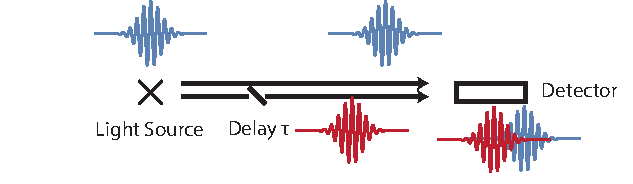
\includegraphics[width=0.8\linewidth]{images/michelson.pdf}
	\caption[Schematic of interferometer]{Schematic of interferometer: Light of (a gaussian) light source with finite coherence time is split and interference with a delayed copy is observed. The time averaged intensity measured by an detector changes with the delay time. }
	\label{fig:michelson}
\end{figure}

\begin{equation}
V=\left|g_1\right|
\end{equation}

Int
-along Glauber/Statistical Optics Goodman



Intensity in double slit leads to normalized degree of coherence $g_1$
Visiblity is modulus of $g_1$.

In a double slit setup (\fref{fig:doubleslit}), $E(r,t)=c_1 E_1(t)+c_2E2(t)$ with complex $c_2$ and $c_2$, $\left|c_1\right|\approx\left|c_2\right|$ describing the propagation to the screen. 

\begin{figure}
	\centering
	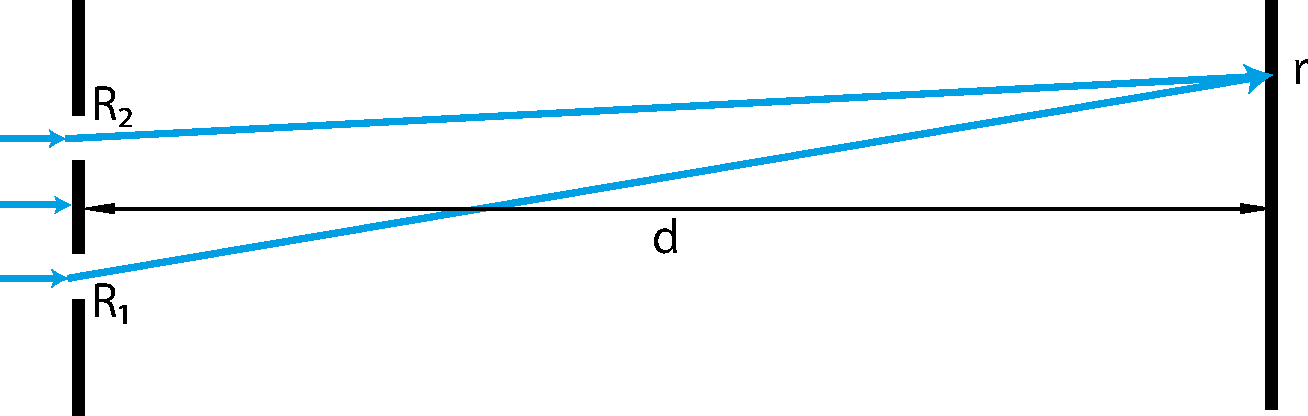
\includegraphics[width=0.8\linewidth]{images/doubleslit.pdf}
	\caption[Schematic of double slit]{Schematic of double slit: Monochromatic light goes through slits located at $R_1$ and $R_2$. The intensity at a position $r$ on the scree (in distance $d$) is the superposition of both paths.  If the slits are within the lateral coherence area of the source, the visibility of the interference pattern depends on the path length difference in comparison to the coherence time $\tau$.}
	\label{fig:doubleslit}
\end{figure}


\paragraph{Second order coherence $g_2(t_1,t_2)$}
The definition of $g_1$ can be extended to the second order by
\begin{equation*}
	g^{(2)}(\vec{r}_1,t_1;\vec{r}_2,t_2= 
	\frac{\left< E^*(\vec{r}_1,t_1)E^*(\vec{r}_2,t_2)E(\vec{r}_1,t_1)E(\vec{r}_2,t_2) \right>}{\left<\left | E(\vec{r}_1,t_1)\right |^2 \right> \left< \left |E(\vec{r}_2,t_2)\right |^2 \right>}	
\end{equation*}
For classical fields normalized correlations of intensities:
\begin{equation}
	g^{(2)}(\vec{r}_1,t_1;\vec{r}_2,t_2)= 
		\frac{\left< I(\vec{r}_1,t_1)I(\vec{r}_2,t_2 \right>}{\left<I(\vec{r}_1,t_1)\right>\left<I(\vec{r}_1,t_1)\right>}	
\end{equation}

\paragraph{Van Cittert Zernicke}
The Van Cittert–Zernike theorem establishes that in the far field, the coherence function of a 
quasi-monochromatic but spatially incoherent light source is proportional to the 2D Fourier transform intensity distribution of the source and Carter and Wolf introduced a generalization for three dimensional sources, showing that in the case of an completely incoherent source field, the complex degree of coherence is proportional to the 3D Fourier transform of the source's intensity distribution \cite{rosen1996, goodman200, carter1981}:
\begin{equation}
	g^{(1)}(\vec{r}_1,\vec{r}_2) \propto I_0^{-1} \int_{S} I_s(\vec{r}) \frac{e^{ik(R_1-R_2)}}{R_1 R_2} \difc \vec{r}
\end{equation}
with the source volume $S$ and intensity distribution $I_s$, total source intensity $I_0=\int I_s(\vec{r}) \difc \vec{r}$ and distances $R_{1,2}=\left|\vec{r}_{1,2}-\vec{r}\right|$. 
%-Hanbury Brown and Twist
\section{Hanburry Brown Twiss}
Hanburry Brown and Twiss 


\paragraph{Siegert Relation}
For thermal light, 
\begin{equation}
	g_2(\vec{r_1},\vec{r_2}) = 1+ |g_1(\vec{r_1},\vec{r_2}) |^2 ,
\end{equation}
which is called the Siegert Relation.
For $N$ Single-Photon-Emitters, a similiar form holds \cite{classen2017}:
\begin{equation}
	g_2(\vec{r_1},\vec{r_2}) = 1+ |g_1(\vec{r_1},\vec{r_2}) |^2 - \frac{2}{N} ,
\end{equation}
As, as according to the van Cittert Zernicke theorem \fref{eq:vcz}, $g_1$ encodes structural information, 
\begin{equation}
g_1(\vec{k_1},\vec{k_2}) \propto \mathscr{F}S(\vec{r}) = S(\vec{q})
\end{equation}
the difference of the intensity-intensity correlation from unity is proportional (with a contrast determining constant $\beta$) to the Fourier transform of the arrangement of emitters with $q=\vec{k_1}-\vec{k_2}$ (see \fref{fig:scatteringvectors}).
 \begin{figure}
	\centering
	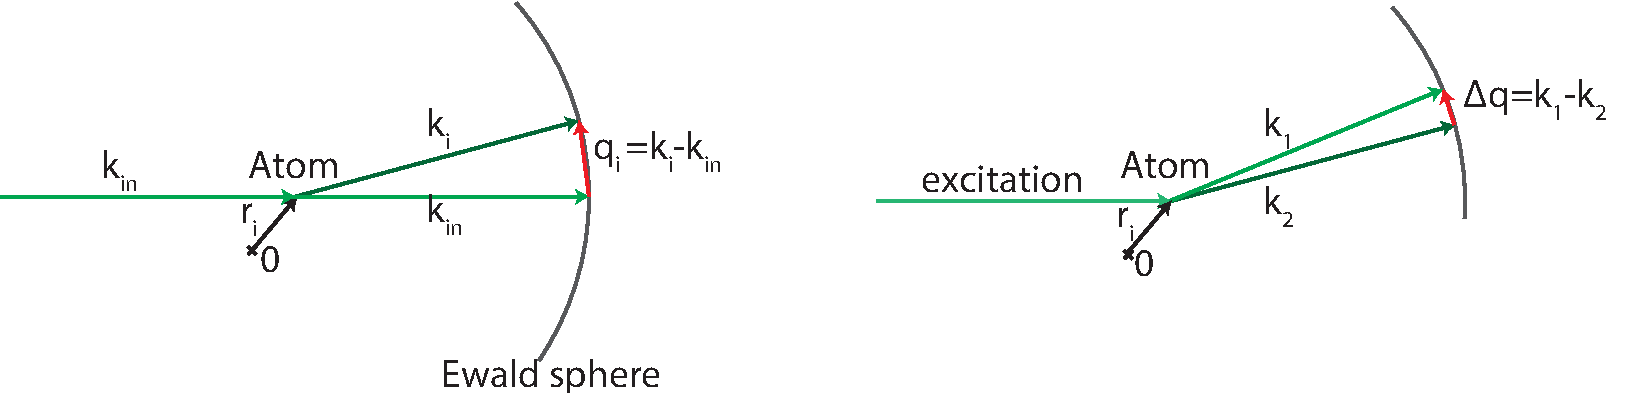
\includegraphics[width=0.9\linewidth]{images/scatteringvectors.pdf}
	\caption[Scattering Vectors]{Scattering vector $q$ in CDI (left) and IDI (right). In CDI, $q$ is the momentum transfer between incoming and outgoing wave. In IDI, there is no momentum transfer from the incoming to the outgoing wave. Instead, intensity correlations of different $k_1$, $k_2$ give a momentum transfer $\delta q$ according to the Siegert relation.}
	\label{fig:scatteringvectors}
	
\end{figure}

%-Single Photon Emitters/2nd Quant description
%(siehe Referenzen in Schaller/resonance fluorescence)
%-Fluorescence g2
%$2 Level with finite Lifetime -> Spectrum of fluorescence
\section{X-Ray Fluorescence}
 \begin{figure}
	\centering
	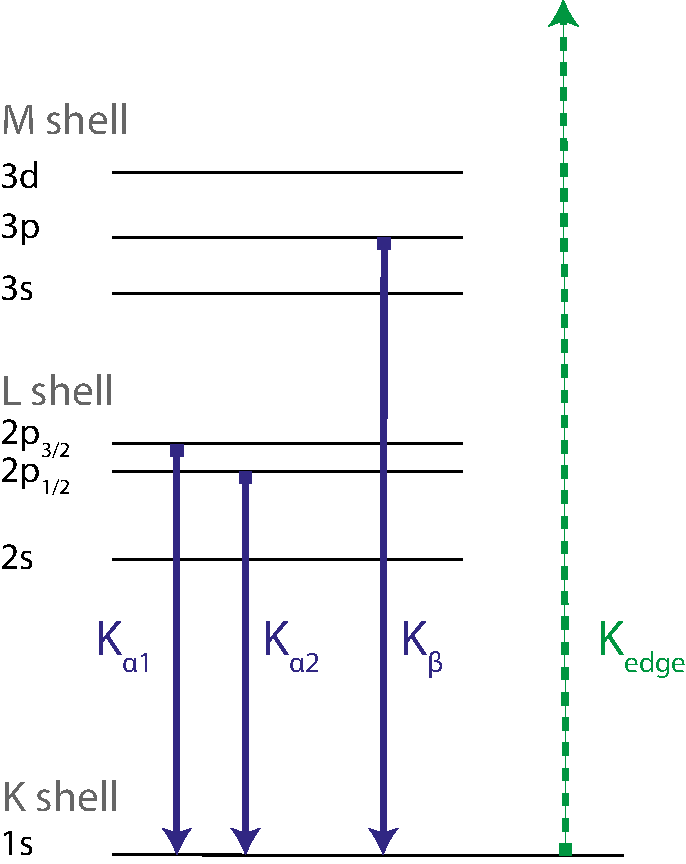
\includegraphics[width=0.4\linewidth]{images/levels.pdf}
	\caption[Atomic Levels]{Atomic levels and associated X-Ray energies}
	\label{fig:levels}
\end{figure}


\begin{table}[]
	\caption[X-Ray Energies]{X-Ray Energies of some relevant elements. }
	\small
	\begin{tabular}{l|l|ll|lll|ll}
		\hline
		Element & K$_{edge}$                                             & \multicolumn{2}{c}{K${_\alpha 1}$}                                                                           & \multicolumn{3}{c}{K${_\alpha 2}$}                                                                                                                                       & \multicolumn{2}{c}{K${_\beta 1,3}$}                                                                              \\
		& \begin{tabular}[c]{@{}l@{}}Energy \\ / eV\end{tabular} & \begin{tabular}[c]{@{}l@{}}Energy \\ / eV\end{tabular} & \begin{tabular}[c]{@{}l@{}}FWHM \\ / eV\end{tabular} & \begin{tabular}[c]{@{}l@{}}Energy\\  / eV\end{tabular} & \begin{tabular}[c]{@{}l@{}}FWHM \\ / eV\end{tabular} & \begin{tabular}[c]{@{}l@{}}rel. \\ Intensity\end{tabular} & \begin{tabular}[c]{@{}l@{}}Energy\\ / eV\end{tabular} & \begin{tabular}[c]{@{}l@{}}rel. \\ Intensity\end{tabular} \\ \hline
		Fe      & 7112                                                   & 6403.8                                                 & 1.61                                                 & 6390.8                                                 & 1.62                                                 & 0.50                                                      & 7058.0                                                & 0.17                                                      \\
		Cu      & 8979                                                   & 8,047.8                                                & 2.11                                                 & 8,027.8                                                & 2.17                                                 & 0.51                                                      & 8905.3                                                & 0.17                                                      \\
		Ga      & 10367                                                  & 9251.7                                                 & 2.59                                                 & 9224.8                                                 & 2.66                                                 & 0.51                                                      & 10263.9                                               & 0.71                                                      \\
		As      & 11867                                                  & 10543.7                                                & 3.08                                                 & 10508.0                                                & 3.17                                                 & 0.51                                                      & 11724.3                                               & 0.19                                                      \\ \hline
	\end{tabular}
\end{table}
\section{Intensity Correlations using X-Ray Fluorescence}
\section{Signal to Noise Considerations}


The noise in the measurement will consist of three parts: First, noise inherent to IDI caused by the random distribution of phases, second, the poissonian noise caused by quantized photons and third, meassurment noise caused by an imperfect detector.

Which factors influence SNR
-lifetime/pulsewidth
-polarisation
-sampling conditions / undersampling
-sample thickness / coherence length
-N images
-N photons



The speckle contrast $\beta$ is governed by the number of independent modes $M$ overlaid in the measurement \cite{goodman2000}.
\begin{equation}
\beta =\tfrac{1}{M}
\end{equation}

If the measurement is performed over a finite amount of time the number of temporal degrees of freedom is
\begin{equation}
M_t=\frac{\left(\int_{-\infty}^{\infty} P(t)\diff t\right)^2}{\int_{-\infty}^{\infty} K(t) \left|\mu(t)\right|^2\diff t}
\label{eq:modes}
\end{equation}
with $P(t)$ the integration window weighting function and $K(t)$ its autocorrelation \cite{goodman2007}. If the integration windows is set by the integration time $T$ of the detector, $P(t)$ is a rectangular function with the width $T$ and
\begin{align}
M_t,rect =T \left[\int_{-\infty}^{\infty} \Lambda\left(\frac{t}{T}\right) \left|\mu(t)\right|^2 \diff t \right]^{-1} .\\
\text{with  }\Lambda(x) = \begin{cases} 
 1-\left|x\right|& \textit{if }|x|<1\\
0 & \textit{otherwise}\\ 
\end{cases}
\label{eq:modesapprox}
\end{align}
Considering the case of a long integration time, $T\gg\tau$, this can be approximated as $M\approx\frac{T}{\tau}$. For a short integration time,  $T\ll\tau$, the number of temporal modes $M$ approaches unity.

If the Integration time can be considered as infinite and instead $P(t)$ is a Gaussian excitation pulse with FWHM of $2\sigma\sqrt{2\ln2}$ and unit area convoluted with an exponential decay with lifetime $\tau$ \cite{butz2015},
\begin{align}
P(t)&=\frac{1}{\tau\sigma\sqrt{2\pi}} \int_0^{\infty} e^{-\frac{t^{\prime}}{\tau}} 
e^{-\frac{(t-t^{\prime})^2}{2\sigma^2}}\diff t^{\prime}
=\frac{1}{2\tau}e^{-\frac{t}{\tau}+\frac{\sigma^2}{2\tau^2}}
\erfc\left[
\frac{\sigma}{\sqrt{2}\tau}
-\frac{t}{\sqrt{2}\sigma}
	\right] ,
	\label{eq:pfull}
	\end{align}
	with the complementary error function $\erfc=\frac{2}{\sqrt{\pi}}\int_x^\infty e^{-z^2}\diff z$, the mode number gets more complicated to evaluate. An approximation can be made if the pulse length is long in comparison to the coherence time, simplifying the autocorrelation of $P$ to
\begin{align}
K(t)=\int_{-\infty}^\infty \frac{1}{4
	\tau ^2}e^{-\frac{t^2}{2 \sigma ^2}-\frac{(t+t')^2}{2 \sigma ^2}}
\erfcx\left(\frac{\sigma^2 -t \tau }{\sqrt{2} \tau \sigma}\right)
\erfcx\left(\frac{\sigma^2 -\tau  (t+t')}{\sqrt{2} \tau \sigma }\right) \diff t'&\stackrel{\tau \rightarrow 0}{\approx} \frac{1}{2\sqrt{\pi}\sigma} e^{-\left(\frac{t}{2\sigma}\right)^2} 
\end{align}
with the scaled complementary error function\footnote{To numerically evaluate \fref{eq:pfull} and integrals involving it, the introduction of the scaled complementary error function  and switching to a sufficient approximation is necessary to avoid under- or overflow of the numerical representation of either the exponential or the error function term.} $\erfcx(x)=e^{x^2}\erfc(x)\stackrel{x\gg1}{\approx}  \frac{1}{\sqrt{\pi}x}$
   \cite{ren2007}.
The number of degrees of freedom in this approximation is
\begin{align}
M_t,gauss&=\left[\int_{-\infty}^{\infty} K(t) \left|\mu(t)\right|^2\diff t\right]^{-1}.
\label{eq:modesapprox2}
\end{align}
For a Lorentzian spectrum (see \fref{eq:docdecay}), the numerical solution of \fref{eq:modes} and the approximations introduced in \fref{eq:modesapprox} and \fref{eq:modesapprox2} is shown in \fref{fig:modes} 

\begin{figure}
	\centering
	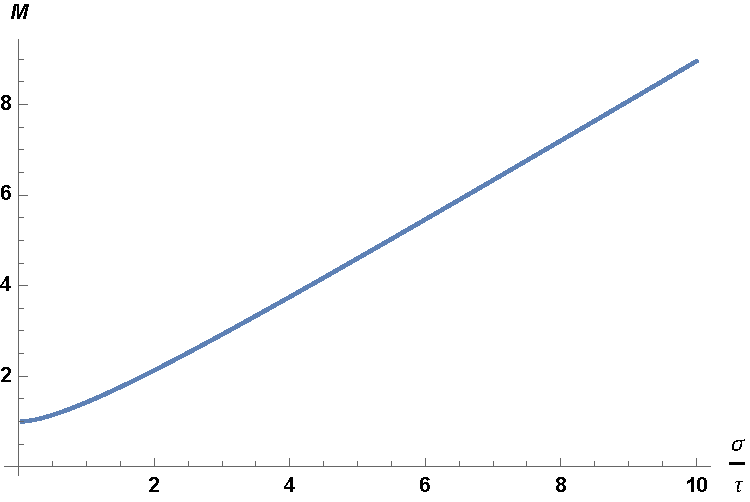
\includegraphics[width=0.5\linewidth]{images/modes_plot.pdf}
	\caption{Temporal Modes}
	\label{fig:modes}
\end{figure}

The experimentally indistinguishable fluorescence energies $K_\alpha,1$ and $K_\alpha,2$ (as well as  $K_\beta$ if no filter is used for suppression) give additional independent modes $M_E$

As the used X-ray detectors are polarization insensitive and X-ray fluorescence is unpolarized and the incoherent field can be separated into two polarization modes, which are pairwise orthogonal with $\vec{k}$ and therefore change slightly for each atom and detector position. For small source dimensions, this change is negligible,  giving $M_P \approx 2$. 


Path differences longer than the coherence length give additional modes $M_S$, therefore the speckle visibility will be reduced for large samples:

If the speckle pattern is not spatially resolved by the detector because its resolution is to low compared to the change in intensity, undersampling will occur, the meassured signal will be spatially averaged giving independent sampling modes $M_D$





As an approximation, the total number of modes can be considered the product of those modes different numbers discussed above, even though in reality, the mode numbers are not completely independent.
Therefore, in \fref{chap:simulation}  simulations under different conditions with experimentally feasible  parameters will be performed.
%- SNR
%will use Peak/stdev bg definition


\label{chap:theory}


\section{Statistics}
Consider a complex sum of phasors of constant amplitude $A$ and independent uniformly in $(-\pi,\pi)$distributed phases $\phi_k$,
\begin{align}
c=\sum^N_k A e^{i\phi_k}
\end{align}
For sufficiently large numbers of $N$, the real and imaginary parts
\begin{align*}
r&=\Re c =  A \sum^N_k \cos(\phi_k)\\
i&= \Im c =A \sum^N_k \sin(\phi_k)
\end{align*}
will (by Central Limit Theorem) be Gaussian random variables with zero mean and variance $\sigma^2=\frac{N}{2}A^2$ and the probability distribution of the amplitude $a=\sqrt(a^2+i^2)$ will  therefore be the Rayleigh distribution
\begin{equation}
p(a)=\frac{1}{2\pi\sigma^2} a e^{\frac{a^2}{2\sigma^2}}
\end{equation}
and  $I=\left|a\right|^2$ will  follow an exponential distribution
\begin{equation}
\label{eq:expdistr}
p(I)=\frac{ e^{-I/\overline{I}}}{\overline{I}}
\end{equation} 
with mean $\overline{I}$ and standard deviation $\sigma=\overline{I}$  \cite{goodman2000,goodman1976}.
A sum of $M$ uncorrelated random variables following identical distributions given by \fref{eq:expdistr} follows a Gamma distribution,
\begin{equation}
\label{eq:gammadistr}
p(I)=\frac{I^{M-1} e^{-I/\overline{I}}} {\overline{I}^M \Gamma(M)},
\end{equation}
for a positive integer $M$ this simplifies with $\Gamma(M)=(M-1)!$ to an Erlang distribution  \cite{forbes2010,trost2020}.
If $I$ is distributed like \fref{eq:gammadistr} and furthermore Poisson sampled as discrete $k$ (such as photon counts), it follows  an negative binomial distribution,
\cite{trost2020,mandel1959,holmes2019}
\begin{equation}
p(k)=
\frac{\Gamma(k+M)}{\Gamma(M)\Gamma(k+1) }
\left( 1+\frac{1}{\overline{I}}
\right)^{-k}
\left( 1+\overline{I}
\right)^{-M}
\end{equation}
with mean $\mu=M\overline{I}$ and variance $\mu+\frac{\mu^2}{M}$ (which differs from the variance of a poisson distribution $\mu$).

This probability distribution can be compared to an experimental measured photon count distribution and the number of modes present in the measurement can be estimated by a regression \cite{lehmkuhler2014,yun2019}.

The variance of a product of (uncorrelated) photon counts  following this distribution will have a variance of
\begin{equation}
\Var_{p\cdot p}= \Var_p^2 +2 \mu^2\Var_p	= \mu^4 \frac{2 M + 1}{M^2 + 2}+ \mu^3 \frac{M+1}{M} + \mu^2 \,.
\end{equation}

Following the idea of Trost et. al, this can be used so estimate the noise of an intensity correlation measurement, even though the actual signal will break the assumption of having uncorrelated photon counts \cite{trost2020}.
\begin{figure}
\centering
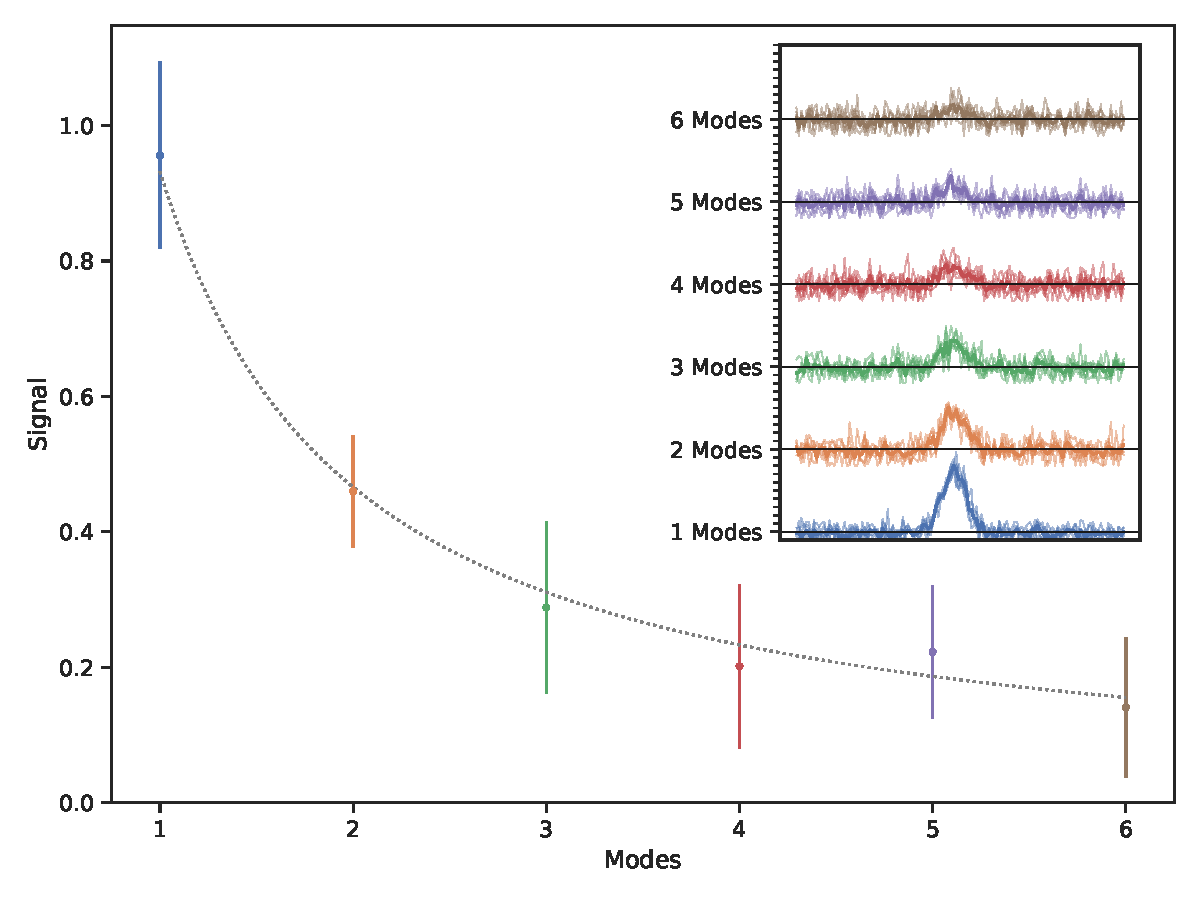
\includegraphics[width=0.6\linewidth]{images/modes.pdf}
\caption[Photon Statistics with different numbers of Modes]{Photon statistics with different numbers of modes $M$ and equal mean of 0.1\,photons. A lower number of modes corresponds the an higher probability of observing multi photon events. The limit of a high number of modes is a Poisson distribution.}
\end{figure}
\section{Kossel Lines}
X-Ray radiation originating from within a single crystal gets Bragg reflected at the lattice planes, causing Intensity variation in $90^o-\theta$ around the direction $k_{hkl}$, forming the \textit{Kossel Cones}. On the spherical detector centered at at the crystal, the points with influenced intensity would lie on circles with radii determined by ...

The visibility of the Kossel lines is governed by the same extinction rules as for the Bragg reflexes for, the structure factor $F_{hkl}$ has to be non-zero. For a zinc blende structure (such as GaAs) with atomic scattering factors $f_a$ and $f_b$, the structure factor is
\begin{align}
F_{hkl} = \begin{cases}
0, & \text{if $h$, $k$, $l$ mixed parity}.\\
4(f_a+f_b), & \text{if same parity and $h+k+l = 4 N$} \\
4(f_a\pm i f_b), & \text{if same parity and $h+k+l = 2 N+1$} \\
4(f_a-f_b), & \text{if same parity and $h+k+l = 4 N+2$} \\
\end{cases}
\end{align}

The structure of the intensity variations (both intense and less intense depends on the which case...
If the fine structure cannot be resolved

The Kossel lines allow to orient the detector with regards to the lattice planes. This can either be done by reprojecting the planar detector onto a sphere by an inverse gnomonic projection and determining circle center and radius, eg. by an Hugh-Transform, or by a fitting conic sections to the lines on the planar detector. As the observable curvature of the Kossel lines on the detector in an IDI setup is small and therefore the circles are difficult to determine, the second method will be used. 

As each point identifyed as beloning to a Kossel line has to be part of a conic section of the same plane with each cone originating from the same point, each point $r$ on a line has to fullfill



\begin{equation}
\frac{\vec{r} \cdot \vec{q}}{\left|\vec{r}\right| \left| \vec{q}\right|} = \frac{\lambda}{2d}
\end{equation}
 for a reciprocal lattice vector $q$ which is an element of the allow reflections $Q$. So finding the dector orientation can be seen as finding a rotation Matrix $R$ as
\begin{equation}
\arg\!\min_{R} \sum_{r} \min_{q\in Q} \frac{2 d * \vec{r} \cdot \vec{Rq}}{\left|\vec{r}\right| \left| \vec{q}\right|} -\lambda
\end{equation}
\begin{figure}
	\centering
	\begin{subfigure}[b]{0.25\textwidth}
	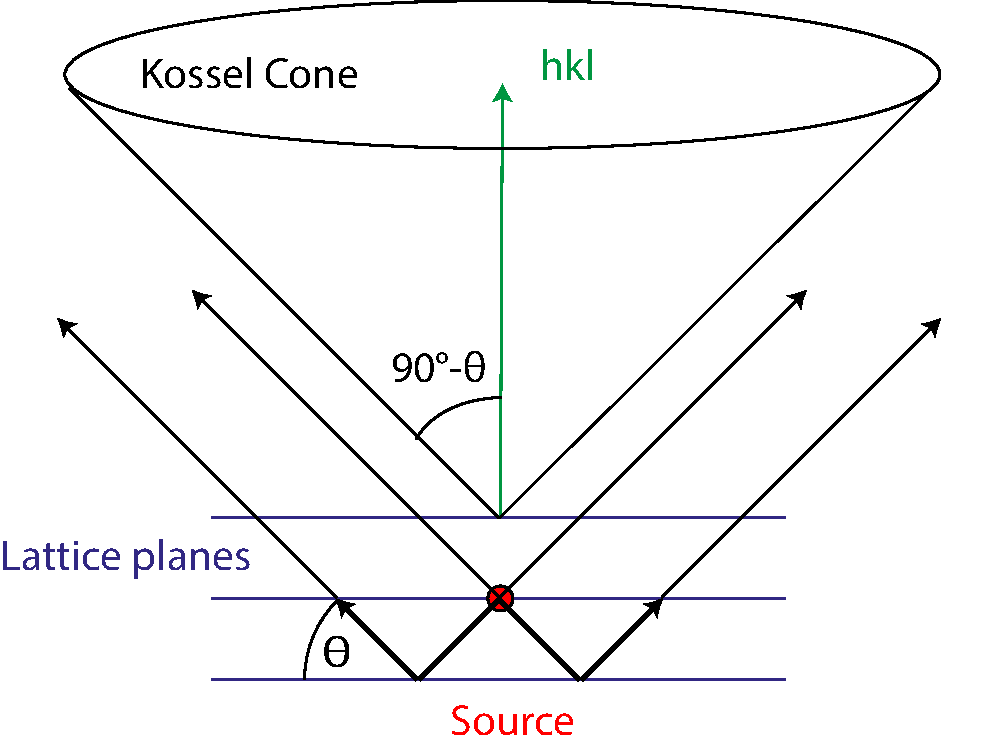
\includegraphics[width=\linewidth]{images/kossel0.pdf}
	\end{subfigure}
	\begin{subfigure}[b]{0.25\textwidth}
	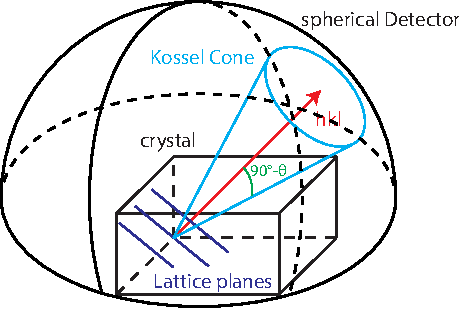
\includegraphics[width=\linewidth]{images/kossel.pdf}
	\end{subfigure}
	\begin{subfigure}[b]{0.35\textwidth}
	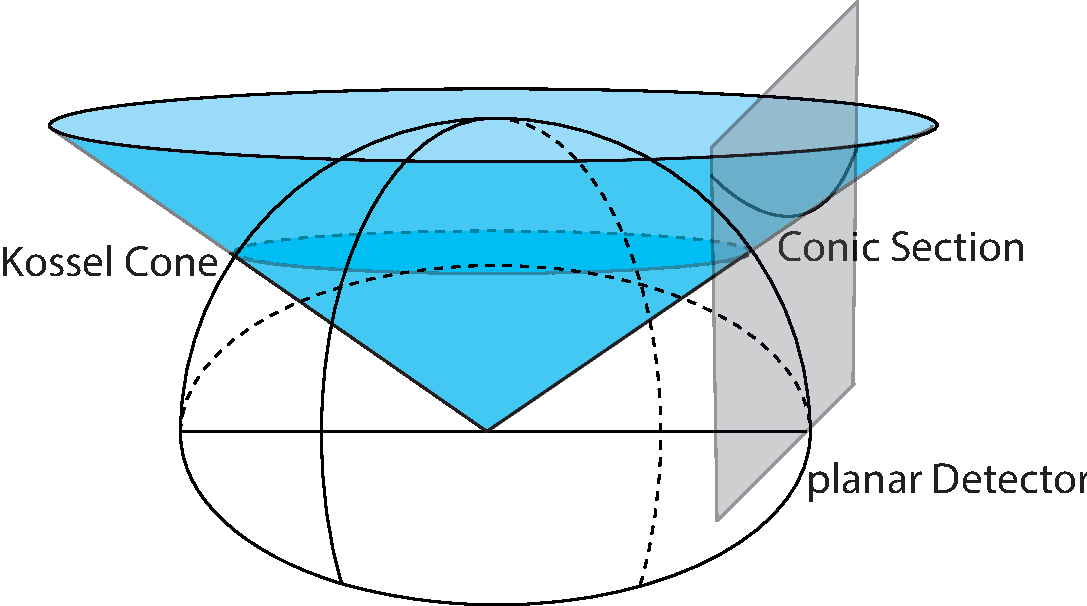
\includegraphics[width=\linewidth]{images/kossel2.pdf}
	\end{subfigure}
	\caption[Geometry of Kossel Lines]{Geometry of Kossel Lines: Radiation from within a light source within a single crystal gets scattered at the lattice planes, causing a change in intensity along a cone of opening angle $90^o-\theta_{hkl}$ and vertex hkl (left). On a spherical detector centered around the sample, those intensity changes would be visible as circular Kossel lines (center). On a planar detector, the intersections of the Kossel cones are visible as conic sections (right)}
	\label{fig:doubleslit}
\end{figure}
\chapter{Simulations}
\label{chap:simulation}
To illustrate the working principle of IDI and to examine the Signal-to-Noise  characteristics, different simulations were performed:

First, it was assumed that the object to be imaged consists of discrete emitters, each emitting monochromatic spherical waves with the same wavelength, but with a randomly chosen phase, and the speckle image on a pixelated detector was simulated by addition of the scalar electric fields and taking the squared magnitude for each pixel. To reduce the influence of this discrete sampling on the simulated speckle patterns, the simulation is performed at XX the resolution and downsampled, such that each data point is the result of 4x4 discrete calculations
In this configuration, the speckle images of a single particle with randomly positioned emitters inside (approximating a single particle imaging setup), a focal volume filled with randomly positioned (non intersecting) hard spheres consisting of randomly positioned atoms (approximating for example many spherical nano particles imaged simultaneously) as well as a crystalline structure with emitters positioned at within a lattice were simulated. In the first two cases, a small-angle regime was chosen and the reconstruction was performed in 2D and as a 1D radial profile. For the crystalline structure, a realistic lattice constant in the same order of magnitude as the K$\alpha$ wavelength moves the reconstruction out of the small-angle regime and a 3D reconstruction of the reciprocal space was performed.
Additionally, in these simulations the effect of under-sampling was studied.

Second, to examine the influence of the fluorescence lifetime and pulse width, a time-resolved simulation was performed.
The results were compared with the approximation, that the contrast is determined by the product of the different number of modes.

Ultimately, the results of these simulations were used the determine the feasibility of an experimental setup using IDI







\section{Time independent Simulations}
In an infinite coherence time, stationary sources approximation, the simulation of the speckle pattern can be performed time independently the superposition of scaler electrical fields emitted with random phases. The simulation of the intensity at multiple discrete points can be performed in parallel using GPU acceleration, resulting in a simple and fast to evaluate model.







\subsection{Detector effects}
To simulate the influence of detector characteristics charge-sharing and readout noise, an image degradation is performed: After Poisson sampling the simulated speckle image, for each photon an uniform random position within its pixel is chosen as the center of Gaussian distribution with FWHM of 0.15 pixel  (similar to the size of the PSF for MPCCD detectors XXX).
The intensity within one pixel is given by the integral over the Gaussian,
\begin{equation}
	I(\Delta x,\Delta y)=\frac{1}{4} \left(\text{erf}\left(\frac{\sfrac{1}{2}-\Delta x}{\sqrt{2}
		\sigma}\right)+\text{erf}\left(\frac{\sfrac{1}{2}+\Delta x}{\sqrt{2} \sigma}\right)\right) \left(\text{erf}\left(\frac{\sfrac{1}{2}-\Delta y}{\sqrt{2}
		\sigma}\right)+\text{erf}\left(\frac{\sfrac{1}{2}+\Delta y}{\sqrt{2} \sigma}\right)\right)
\end{equation}
with $\sigma$ the standard deviation of the Gaussian in pixels and $\Delta x$, $\Delta y$ the distance of the pixel to the chosen photon center, and evaluated for the neighboring pixels. Afterwards a Gaussian readout noise is added. The effect of this degradation on the spectrum is illustrated in \fref{fig:degrad}.



\paragraph{Photon counting}
As the relevant signal for the correlation analysis is the presence of fluorescence photons, but charge sharing and readout noise of the detector as well as the presence of photons caused by air scattering degrades this signal, different approaches  of preprocessing will be compared:

\begin{itemize}
	\item Using the raw signal
	\item Using the raw signal after applying a threshold.
	\item Discretization by closest number of signal photons
	\item Discretization by closest possible combination for each pixel
	\item Discretization by maximum likelihood
	\item Droplet algorithm
\end{itemize}
The noise thresholding will be done with a threshold of 3$\sigma$. To find the closest number of signal photons, the signal after thresholding is divided by the expected energy of a single photon and rounded to the closest integer. Considering possible combinations of signal and scattering photons by finding  $nE_{fluorescence}+mE_{excitation}$ with integer $n$, $m$ closest to the observed value and only using the signal photon number $n$ for the correlation would suppress the influence of scattering, but would still be influenced by charge sharing and doesn't account for the different probabilities of signal and scattering photons.

If the detector noise level, the PSF due to charge sharing as well as the distribution of signal and scattering is known, a Bayesian classifier can be trained on synthetic data, which each observed value on the detector, returns the number of signal photons with the highest conditional probability (\fref{fig:probs}). Depending on the apriori probabilities and the detector characteristics, this maximum likelihood solution can differ from the closest combination. If those parameters are not known with reasonable certainty, an educated guess can still provide decision boundaries.

\begin{figure}
	\centering
	\begin{subfigure}[b]{0.45\textwidth}
		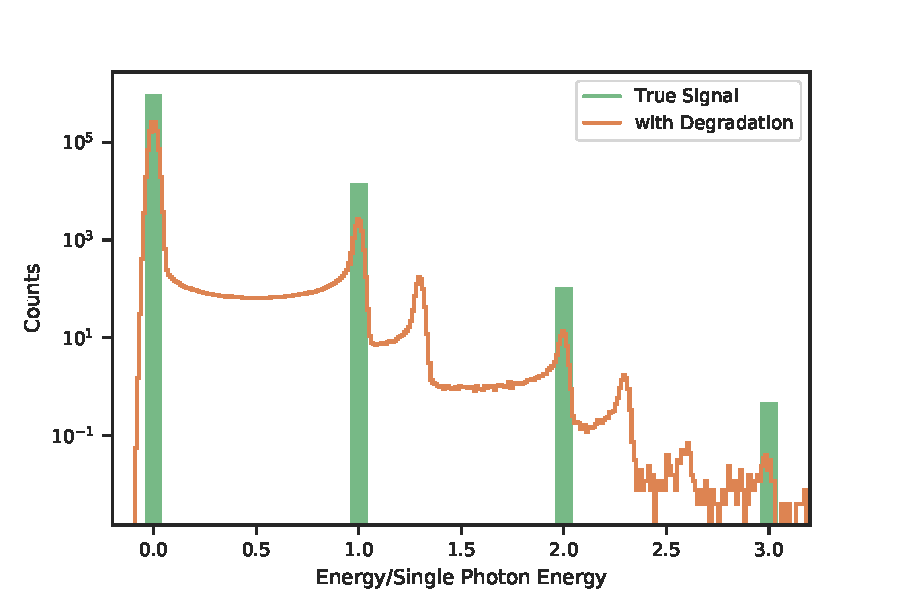
\includegraphics[width=\linewidth]{images/sharing.pdf}
		\label{fig:degrad}
		\caption{True Histogram and Degradation}
	\end{subfigure}
	\begin{subfigure}[b]{0.45\textwidth}
		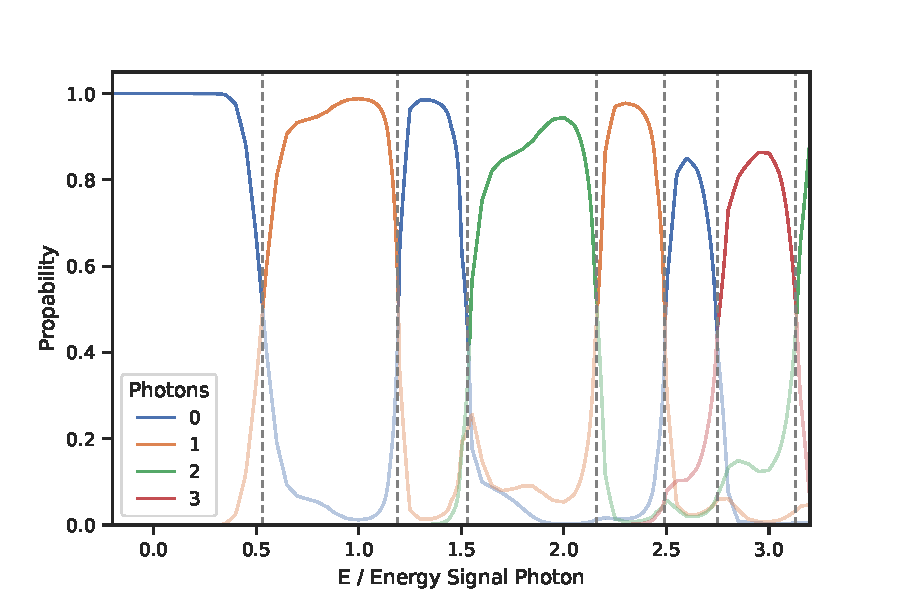
\includegraphics[width=\linewidth]{images/probs.pdf}
		\label{fig:probs}
		\caption{Probabilities and Decision Boundaries}
	\end{subfigure}
	
	\caption[Histogram, probabilities and decision boundaries for the photon number]{For a Poisson distributed signal with mean 0.01 photons/pixel, a Poisson distributed scattering with mean 0.001 photons/pixel and an photon energy of 1.3 times the energy of a signal photon, a charge sharing PSF with $\sigma$ 0.1 pixel and a Gaussian noise with $\sigma$ 0.05 photons, the simulated histogram is shown on the left. Detector noise, charge sharing scattering photons degrade the histogram. The probabilities of an observed energy being caused by a certain number of signal photons is shown on the right, the dashed lines mark the decision boundaries for an Bayesian classifier.} 
\end{figure}


\begin{figure}
	\centering
	\begin{subfigure}[b]{0.85\textwidth}
		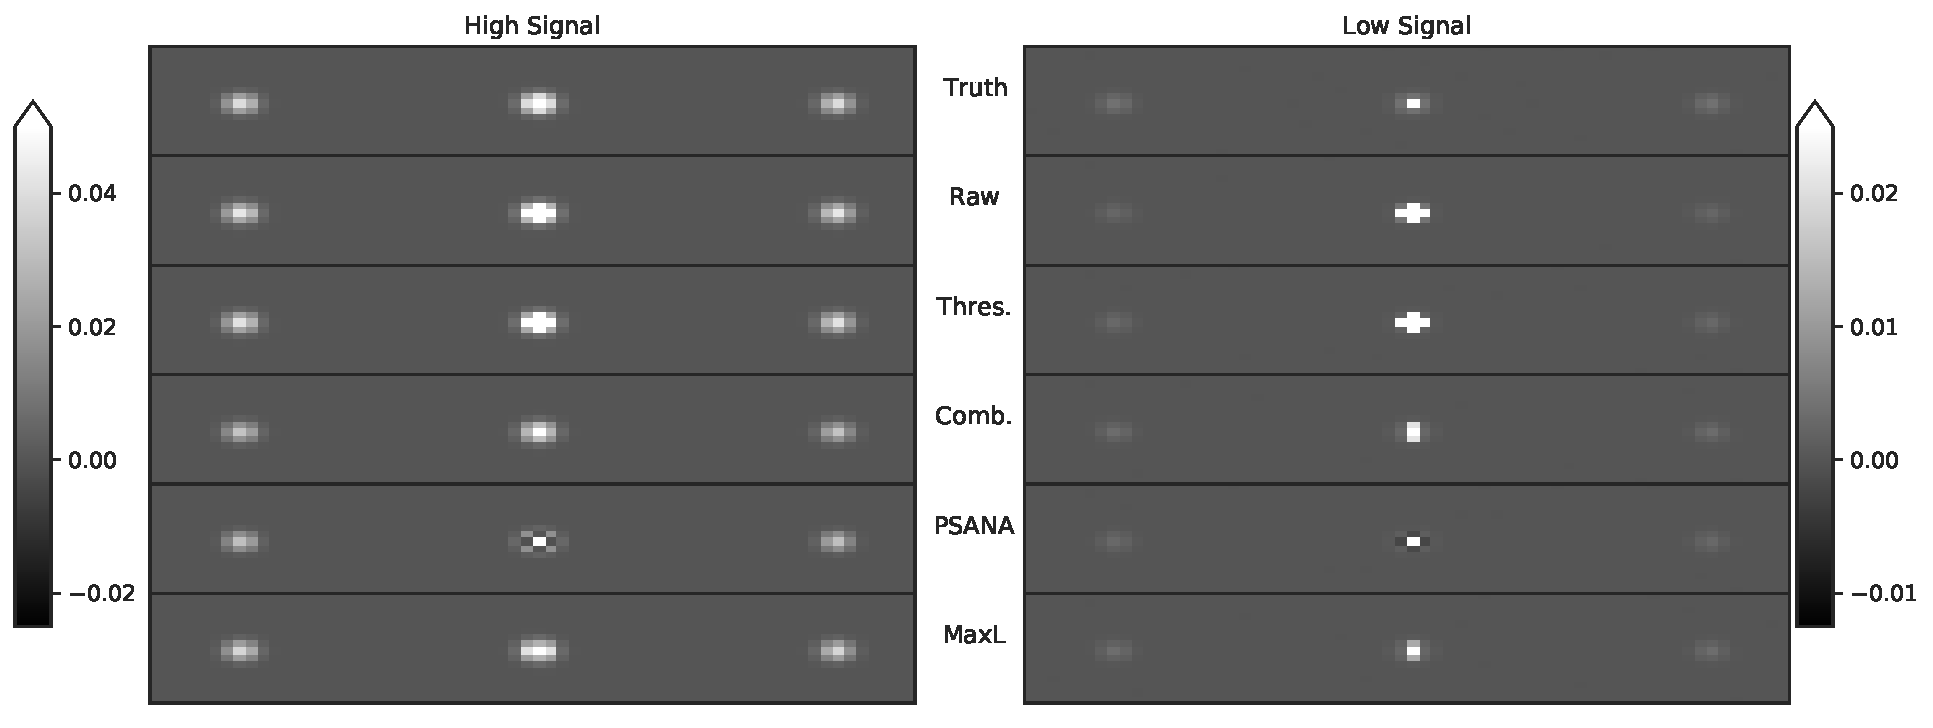
\includegraphics[width=\linewidth]{images/photonreconimg.pdf}
		\label{fig:photonreconimg}
		\caption{Reconstructions}
	\end{subfigure}
\\
	\begin{subfigure}[b]{0.95\textwidth}
		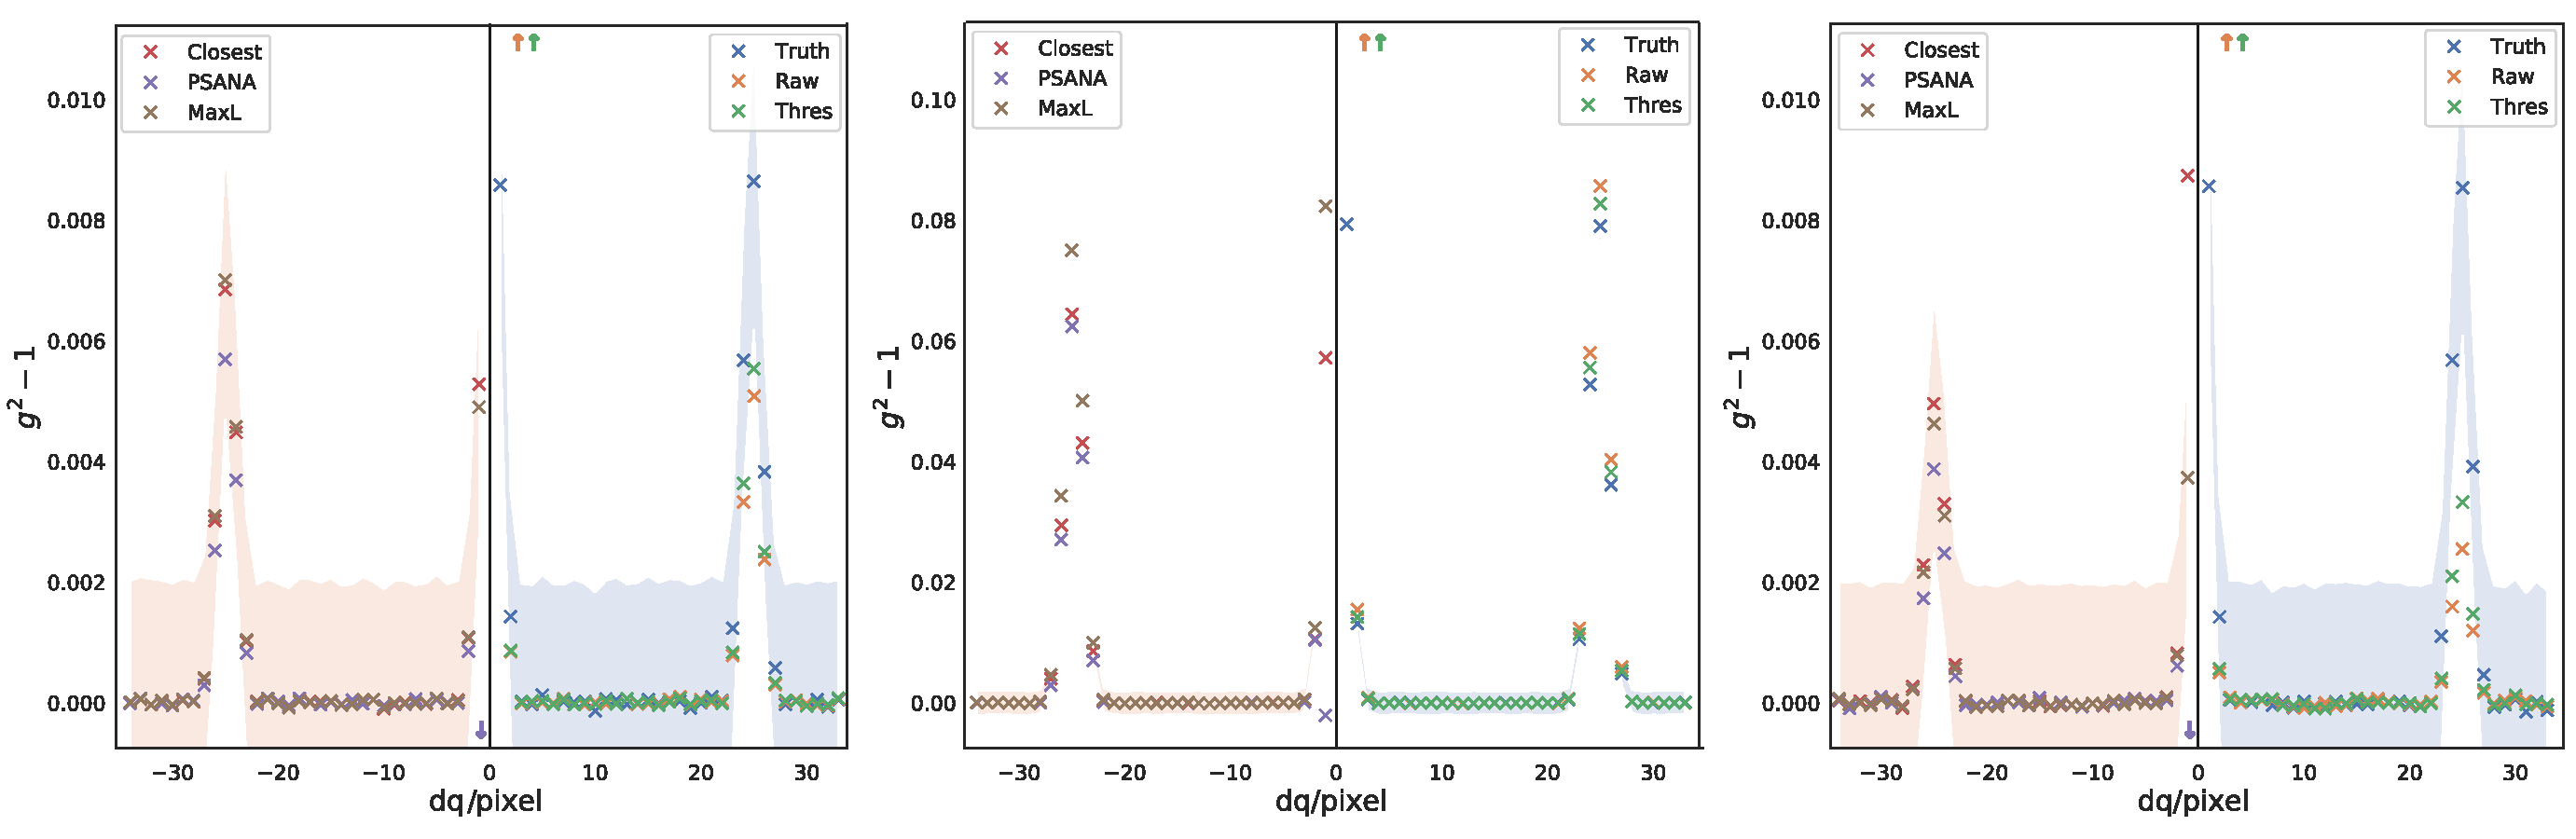
\includegraphics[width=\linewidth]{images/photonrecon.pdf}
		\label{fig:photonrecon}
		\caption{Profiles}
	\end{subfigure}	
	
	\caption{Result} 
\end{figure}





For comparison, the PSANA Photon algorithm, a droplet algorithm considering only the signal photons is used \ref{psana}.

Possible avenues for improvement would be to use a more sophisticated droplet scheme based on error minimization allowing for subpixel resolution, incorporating the scattering photons into the droplet algorithm or using a neural network trained on synthetic images.




\subsection{Normalisation}
Mean of all pixels 
Mean of all pixels inside the overlap

If only a single image is taken, the expectation value for each pixel has to be approximated.

If multiple images are taken, under the assumption of ergodicity, the expectation value for each pixel can be approximated by its mean over many images. To account for fluctuations in the exciting FEL pulse and resulting fluctations of the fluorescence intensity, it can be assumed that the distribution over pixel  intensities and FEL intensities are uncorrelated, and the detection probability of each pixel in each shot can be factorized into the product of the probability to detect a photon in a pixel and to detect a photon in a shot. Therefor, the effect of the FEL intensity fluctuations can be suppressed by normalizing each image by the total intensity of the image.



\subsection{Autocorrelation}

\subsection{Accessible Reciprocal Space}
	\paragraph{Crystal}
	\paragraph{Spherical Samples}


\subsection{Number of images}
\subsection{Undersampling and detector size}
\subsection{Random Orientations}

\subsection{Multiple Samples}
To decide if having more than one spherical sample in the focus is advantageous, an additional simulation is performed:
 
Multiple spheres inside the focal volume, placed randomly but ensuring a minimum distance between neighboring spheres larger than the diameter plus twice the thickness of an additional layer of non-fluorescing organic dispersion agent capping the spheres with no other interaction are simulated.  The number of particles is varied, ranging from a single sphere over multiple spheres to a Poisson Sphere Distribution as a random placement of particles with the minimal allowed spacing and mean a volume fraction of approx. 25\% \footnote{without the buffer layer, the volume fraction would be around 50\%, significantly smaller than the densest possible packing}. 
The structure factor of this ensemble of spherical particles is determined by three factors: The structure factor of the focus, the structure factor of points following an Poisson Sphere Distribution and the structure factor of a single sphere.(see \fref{fig:multisphere1}). As the number of spheres is increased, the influence of the focal volume increases and the distribution of the spheres's centers increases (see  \fref{fig:multisphere2})
For spheres with 20\, nm radius, a spacing layer of 5\,nm around each sphere, with  50000 excited atoms per sphere on average, a focus of 200nm (FWHM), the fluorescence on a 1024x1024 pixel (pixelsize 100\,um) detector placed 30\,cm is simulated. In this geometry, assuming constant distance to the sample for each detector pixel, approximately 1\% of the emitted photons reach the detector. 
For each number of spheres 5000 images are used for an IDI reconstruction.
As the number of photons sphere is kept constant, opposing effects occur:  With increasing number of particles and therefor photons recorded, the Poisson noise is reduced, but the signal strength in low scattering angles is decreased as the structure factor changes from a single sphere to a hard-sphere model. Therefor, for the chosen simulation parameters an optimum in the detectebility of a correlation effect can be found for a medium number of samples in the focus, below


As the number of particles inside the focus is increased, in the low $q$ region of the IDI reconstruction, the focal volume becomes more visible. For high numbers of particles, the structure factor of the distribution of the centers of the particles causes a reduction in the scattering factor in the low $q$ region. For low numbers of particles inside the focus, the Poisson noise casued by the low photon numbers dominates the error.

\
 
\begin{figure}
	\centering
	\begin{subfigure}[b]{0.32\textwidth}
		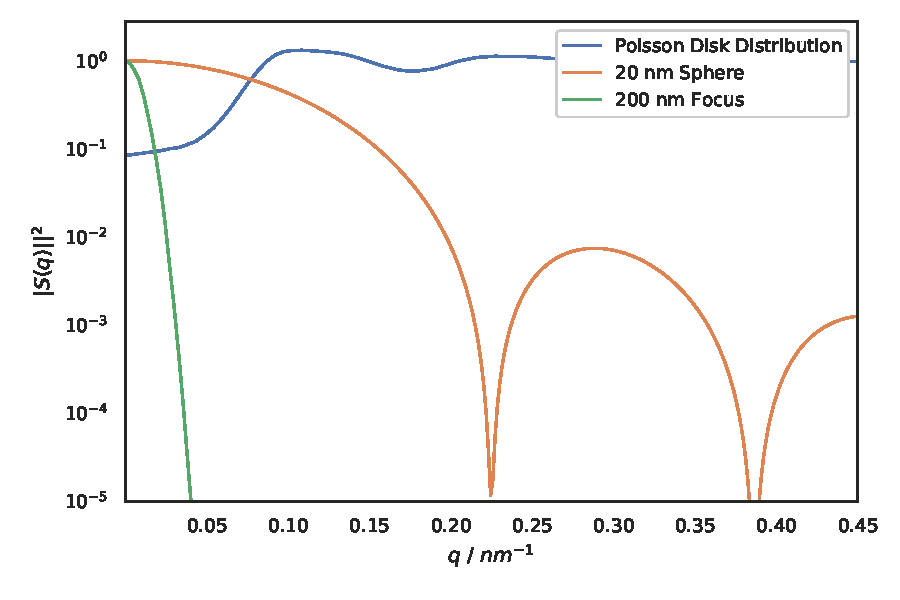
\includegraphics[width=\linewidth]{images/multisphere1.pdf}
		\caption{Structure Factors\\$ $}
	\end{subfigure}
	\begin{subfigure}[b]{0.32\textwidth}
		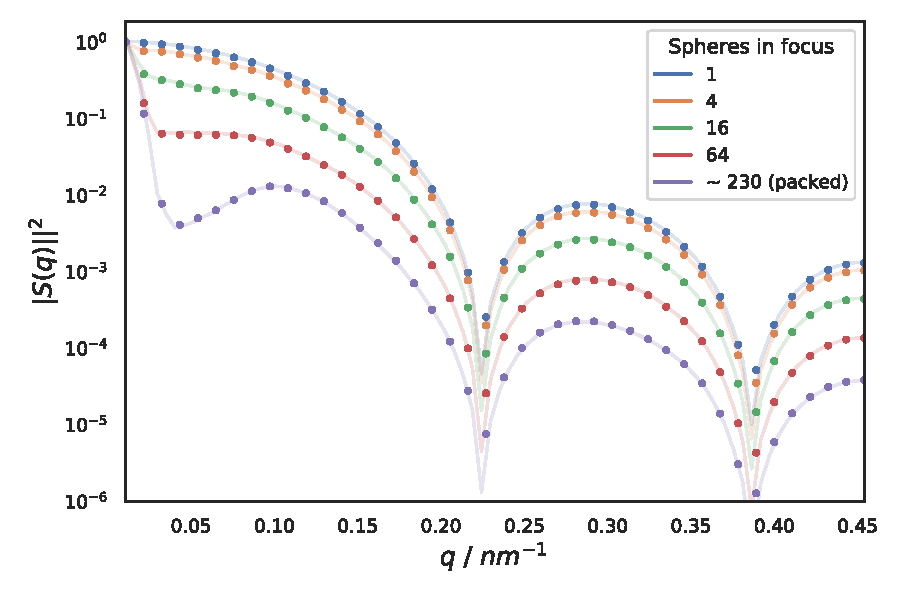
\includegraphics[width=\linewidth]{images/multisphere3.pdf}
		\caption{Structure Factor of Multiple Spheres}
	\end{subfigure}
	\begin{subfigure}[b]{0.32\textwidth}
		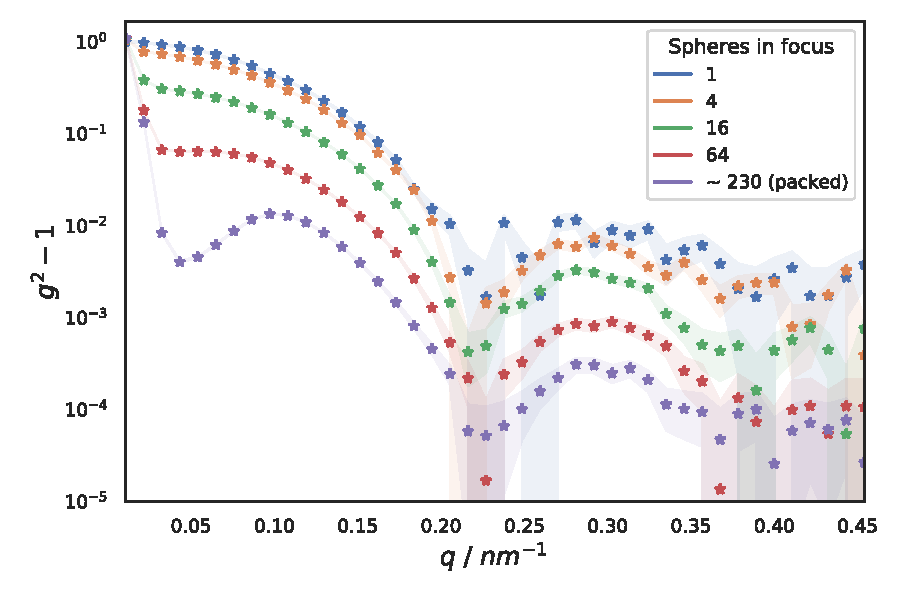
\includegraphics[width=\linewidth]{images/multisphere2.pdf}
		\caption{IDI Reconstruction \\ $ $}
	\end{subfigure}
\caption{Structure factors of a sphere with 20\,nm radius, a 200\,nm Gaussian focus and a random distribution of points at least 50\,nm apart (a), the structure factor of different numbers of hard 20\,nm radius spheres with an additional 5\,nm separating layer on each sphere inside the focal volume (b), and the result of an IDI simulation assuming iron fluorescence, a mean of $5*10^4$ excited atoms per sphere, a 1024x1024 pixel (100\,um pixelsize) detector in a distance of 30\,cm (resulting in approximately 1\% of the emitted photons being captured), and using 5000 images (c). The shaded area is the standard error of the mean over images, the markers show the discrete $q$ steps in the reconstruction.}


\end{figure}

\section{Time dependent Simulations}

Each of the $N$ atoms is assigned an emitting time $t_{n}$ chosen according to the excitation pulse shape and its position. Starting from this emitting time, the atom emits an exponential decaying field with a decay time chosen to match the lifetime. 



For each discrete pixel on the simulated detector, for each atom the distance $d_n$, the arrival time $t'_n=t_n+d_n/c$ of each atom's initial radiance, and its time independent complex field $E_n=\frac{1}{d} e^{ikd_n+\phi_n}$ with initial random phase $phi$ is calculated.
The time dependent E field is the summation over the decaying field of all atoms,
\begin{equation}
E(t)=\sum_{n=1}^N  E_n \Theta(t'_n  - t) * e^{-(t-t'_n )/\tau}
\label{eq:tdsum}
\end{equation}
and the simulated intensity the time integral over the magnitude squared of the E-field,
\begin{equation}
I=\int_0^\infty \left| E(t) \right|^2 .
\label{eq:tdint}
\end{equation}

To efficiently solve this integral for each detector pixel, it can be split into N parts with a constant number atoms which radiations have already arrived, and each of those parts can be solved analytically. For this, first all atoms are sorted by the arrival time at the pixel. At each arrival time $t'_n$, the sum in \fref{eq:tdsum} gets a new term and the field is calculated as
\begin{equation}
E(t_n)=E(t_{n-1})*e^{\sfrac{t_{n-1}-t_n}{\tau}}+E_n
\end{equation}
 This can be done with a parallel inclusive scan, as shown in \fref{algo:td}. This gives the supports for the integral, as show in \fref{fig:tdplot}, which can now be solved as
\begin{align}
	I&=\int_0^\infty \left| E(t) \right|^2 = \sum_{n=1}^{N-1} \int_0^{t_{n+1}-t_n} \left|E(t_n)\right|^2 e^{-2t/\tau} \dif t +\int_0^\infty \left| E(t_N)\right|^2 e^{-2t/\tau} \dif t \\
	 &=  \frac{\tau}{2}  \left|E(t_N)\right|^2 -  \frac{\tau}{2}\sum_{n=1}^{N-1} \left|E(t_n)\right|^2 (e^{-2 (t_{n+1}-t_n)/\tau} -1 ) 
\end{align}

This procedure is efficient in regards of discrete time steps that need to be calculated and can easily be run on a GPU.

In \fref{fig:tdpshere} the results of a simulation with Gaussian pulses with different for a single spherical object is shown. The dependence of the speckle visibility and the visibility of the reconstructions is in agreement with the theoretical considerations.

To investigate the influence of sample thickness for crystalline samples as second simulation is performed. As a thicker sample gives more photons and therefore less Poisson noise, but a higher number of temporal and spatial modes and therefore a lower expected lower speckle visibility, a simulation close to experimentally feasible parameters is desirable.



\begin{figure}
	   \centering
		\includegraphics[width=0.7\linewidth]{images/tdplot.pdf}
	\caption[Integration in Time Dependent IDI Simulation]{To illustrate the integration in the time dependent IDI simulation, the (normalized) scalar field at one point of the detector created by 10 emitting atoms with $\tau$=1\,fs and a pulse FWHM of 2\,fs is shown. The solid colors show each atom's field, the line plot the (phase correct) sum. The simplify the calculations, only the time points marked with stars are calculated. To solve the integral \fref{eq:tdint}, it's sufficient to calculated the squared magnitude at those points and to do a piecewise integration from each star-shaped marker the next dot-shaped marker. The color wheel in the top right shows colors used for phase encoding in the plot.}
	\label{fig:tdplot}
\end{figure}


\begin{figure}
	\begin{subfigure}[b]{0.32\textwidth}
		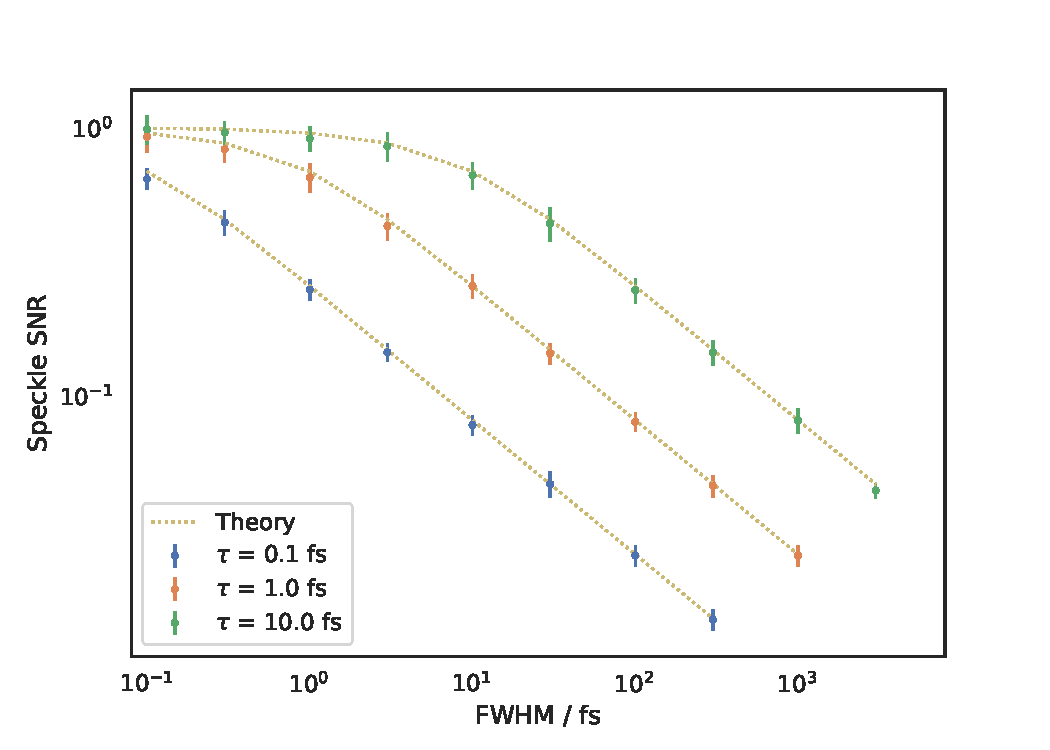
\includegraphics[width=\linewidth]{images/timedependent_1.pdf}
	\caption{Speckle SNR for different pulse FWHM and decay times $\tau$\\$ $}
	\end{subfigure}
	\begin{subfigure}[b]{0.32\textwidth}
		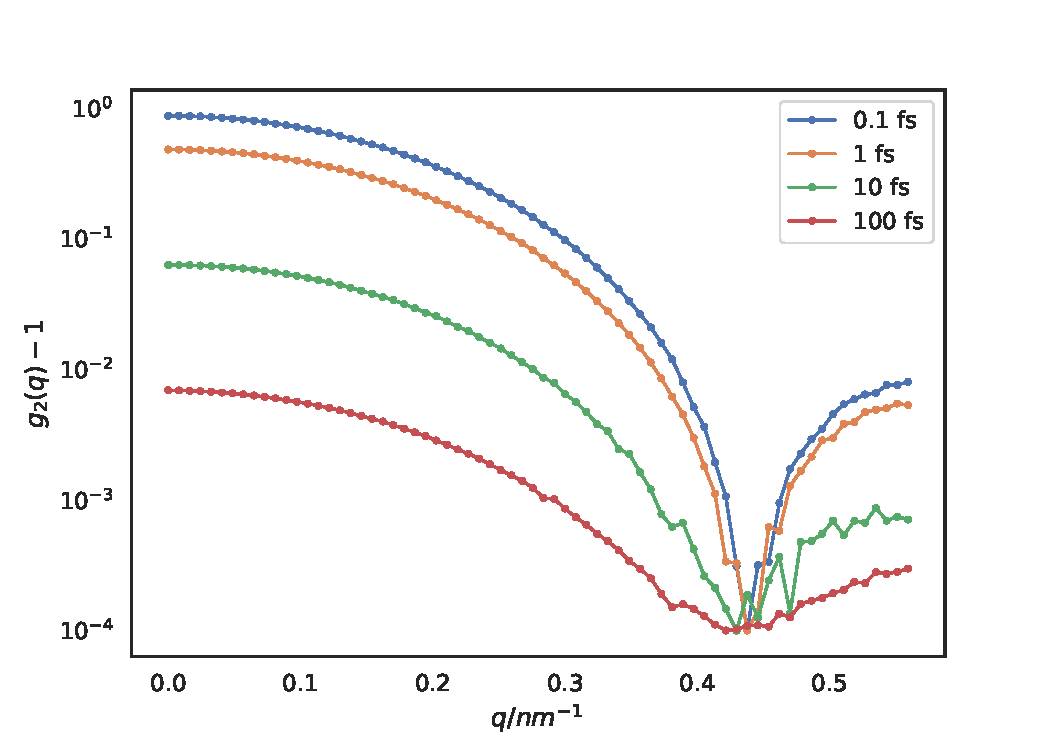
\includegraphics[width=\linewidth]{images/tdsphere.pdf}
		\caption{Reconstructed radial profiles at different pulse FWHM and fixed decay time $\tau = 0.1$\,fs}
	\end{subfigure}
	\begin{subfigure}[b]{0.32\textwidth}
		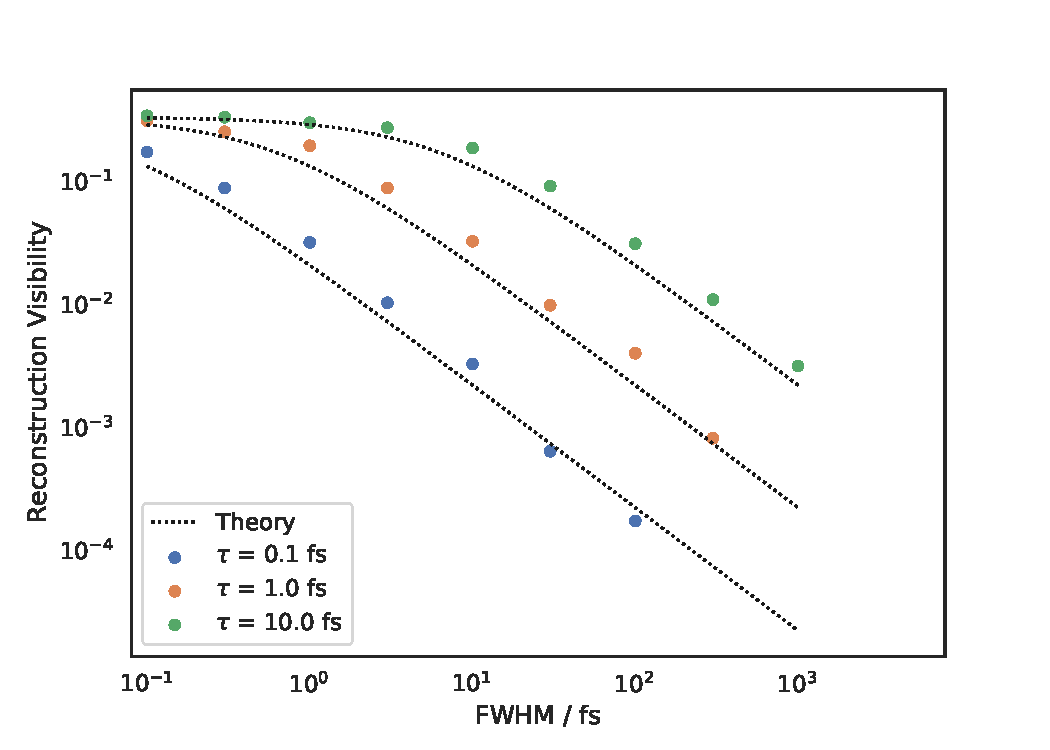
\includegraphics[width=\linewidth]{images/timedependent_2.pdf}
		\caption{Visibility of the reconstruction for different pulse FWHM and decay times $\tau$}
	\end{subfigure}
	\caption[Time Dependent IDI Simulation of a Sphere]{Time Dependent IDI Simulation of a Sphere: For a sphere with 10\,nm radius consisting of $2*10^5$ atoms emitting 6.4\,keV fluorescence captured by an 256x256@50\,um detector in 20\,cm distance, a series of simulations were performed with different decay times $\tau$ of the emission and different exciting pulse FWHM. In a) the SNR of the simulated speckle pattern is compared with the theoretical  $1/\sqrt{erfcx(2\sigma/\tau}$ dependence on the ratio of pulse length and $\tau$. In b) exemplary radial profiles of the reconstruction of 50 images each are shown for one fixed $\tau$. Those reconstructions are used to plot the  dependence of the visibility on the pulse width in c). For long pulses, the reciprocal dependence on the pulse length is visible.}
	\label{fig:tdpshere}
\end{figure}

\subsection{Pulse length}
\subsection{Sample thickness}



\section{Implications for an experimental design}


\chapter{Experimental Verification}
An initial experimental proof of principle experiment was performed at the SACLA FEL.
The experiments consisted of three parts: First, reproducing XXX and imaging projection of the focal volume of the FEL by using metal foils as samples, performing a measurement of the K$\alpha$  fluorescence and an reconstruction in the small angle regime. Second, moving the a smaller length scale and try to image nanoparticles. And Third, leaving the small angle regime and record the fluoresccne of a single crystal and perform a reciprocal space reconstruction.
\section{Sample Preparation}
As an nanoparticle sample, spherical iron oxide nanoparticles where chosen. To improve the number of detected fluorescence photons per FEL shot, the decision was made to have many particles many for each shot within the focus. This ensures a higher number of fluorescence photons recorded and basically eliminates the possibility of having shots without any particles inside the focus. 

Magnetite Nanoparticles coated with Oleic Acid dispersed in Toluene were bought from NN-Labs, inhibited Methylmethacrylate (MMA) and Etyhlhexylmethacrylate (EHMA)  (Sigma Aldrich) were filtered using a prefilled column to remove the Inhibitor,  2,2-azo-bis-isobutyrylnitrile (AIBN) (Sigma Aldrich) was used as thermally activated radical initiator as received. Polystyrene (Sigma Aldrich, MW XXX) was used as received. As solvents, Methanol, Toluene and Chloroform were used.
\subsection{Nanoparticles in Polystyrene Matrix}
The nanoparticles were precipitated with Methanol, centrifuged and redispersed in Chloroform at a concentration of 25\,mg/ml, whereas the weight of nanoparticles includes the weight of the oleic acid capping. Polystyrene was dissolved in Chloroform at a concentration of 250\,mg/ml and different volumes of the nanoparticles solution were added (to account for the different iron contents) to 5\,ml of the Polystyrene solution (see \fref{tab:samplePS}). After ensuring dispersion by strong sonication, fractions of XXX\,ul the solution were dropped onto glass slides and dried. After drying, the approximately 200\,um thick films were carefully removed from the glass slides.
As an iron containing control sample, 60mg FeCl3 and XXX Polystyrene were dissolved in 6ml acetone, sonicated and  fractions of XXX were dropped onto slowly spinning glass slides (XXX rpm for XX 5\,min) and carefully removed after drying.
\begin{table}[tp]
	\centering
	\caption{Nanoparticles in Polystyrene recipes}
	\label{tab:samplePS}
	\begin{tabular}{llll}
		\hline
	NP size&   Volume NP in CF &  Iron Concentration &Volume PS in CF    \\
		\hline
	  5\,nm&700 ul & & 5\,ml  \\  
	   10\,nm&  500 ul& &5\,ml  \\    
	   20\,nm &  425 ul& &5\,ml  \\  
	   	Control   &  & &5\,ml  \\  
		\hline
	\end{tabular}
\end{table}

\subsection{Nanoparticles in Poly(MMA/EHMA)  Matrix}
As a second nanoparticle in polymer sample, a AIBN initiated Poly(MMA/EHMA) polymerisation with magnetite nanoparticles was performed. 
The nanoparticle solution was concentrated to XXX in toluene by precipitation, centrifugation and redispersion. To account for the different iron concentration, to different amounts of the nanoparticle solution and additional toluene, 800\,ul of EHMA was added each (see \fref{tab:sampleCP}). After strong sonication to ensure dispersion, 3.2\,ml of MMA were added and the solution was bubbled with N$_2$ for 5\,min. To start the polymerisation, 20\,mg of AIBN were added and the solution was bubbled again with N$_2$  for 10\,min before heating it up to XXX using a water bath under weak sonication using a sonic bath. The mixture was kept at XXX for XXX.
The vials were uncapped and the polymer dried for 12h at XXX. The polymer was removed from the vials and cut into slices of approximatly XXX thickness using a slow spinning diamond saw.
As a control sample, the polymerisation was performed without any nanoparticles added.

\begin{table}[tp]
	\centering
	\caption{Nanoparticles in PMMA/EHMA recipes}
	\label{tab:sampleCP}
	\begin{tabular}{llllll}
		\hline
		NP size &NP in Toluene&Toluene & EHMA & MMA & AIBN \\
		\hline
		5\,nm& & &800\,ul&  3.2\,ml&   20\,mg    \\
		10\,nm& & &800\,ul&  3.2\,ml&   20\,mg    \\
		10\,nm& & &0\,ul&  4\,ml&   20\,mg    \\
		20\,nm& & &800\,ul&  3.2\,ml&   20\,mg    \\
			Control& & 1\,ml&800\,ul&  3.2\,ml&   20\,mg    \\
		\hline
	\end{tabular}
\end{table}

\subsection{Nanoparticle Sample Characterisation}
Before sample preparation, the iron oxide nanoparticles as received were diluted with Toluene, deposited on a silicon nitride membrane and imaged using a FEI Tecnai microscope  (see \fref{fig:tem}).  For each of the three nominal sizes, 3 different areas on the membrane were analyzed using ImageJ, resulting in mean radii of 8.3$\pm$1.7\,nm ("20\,nm") 4.1$\pm$0.8 \,nm	("10\,nm") 3.1$\pm$0.6\,nm ("5\,nm"). In the TEM images, the effect of the oleic acid ligands used to stabilize the nanoparticle dispersion  can be seen as the inter-particle distance.

\begin{figure}[tp]
	\centering
	\begin{subfigure}[b]{0.3\textwidth}
		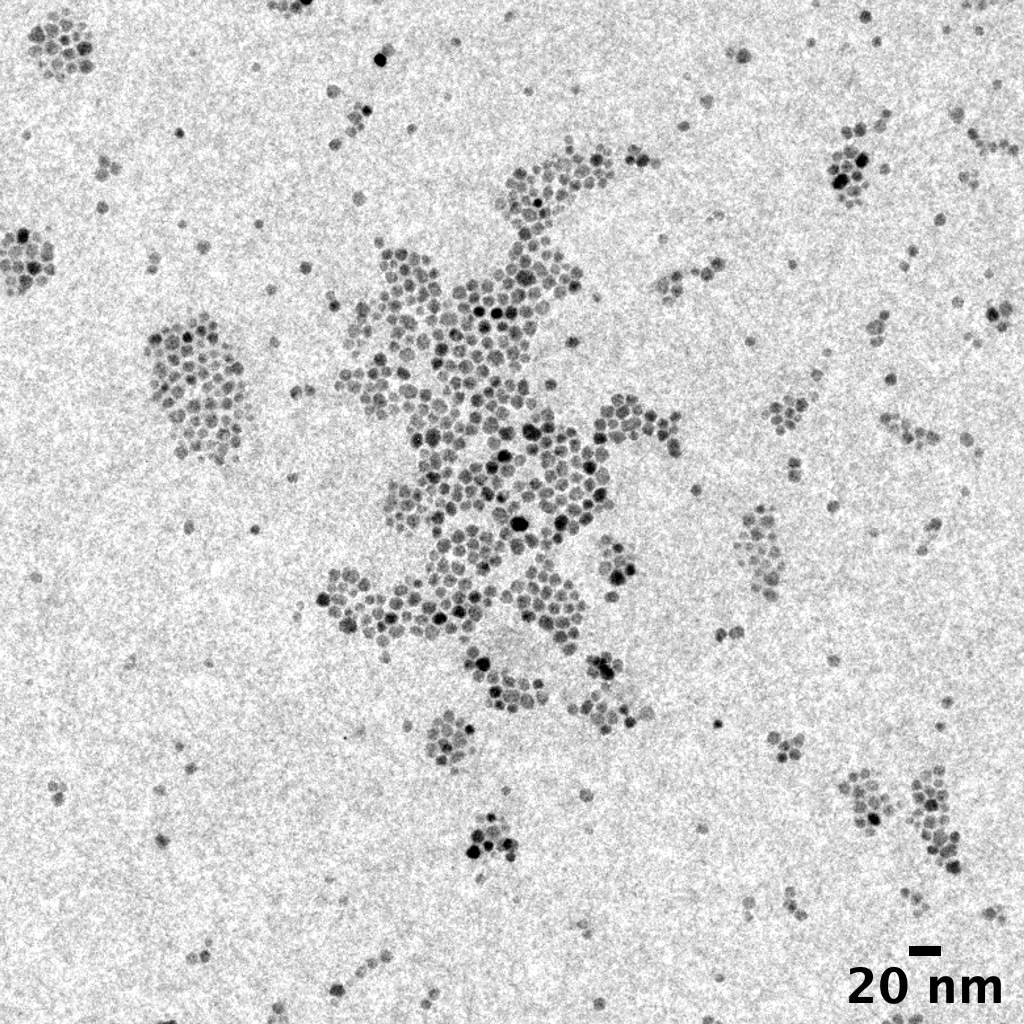
\includegraphics[width=\linewidth]{images/tem5.png}
	\end{subfigure}
	\begin{subfigure}[b]{0.3\textwidth}
		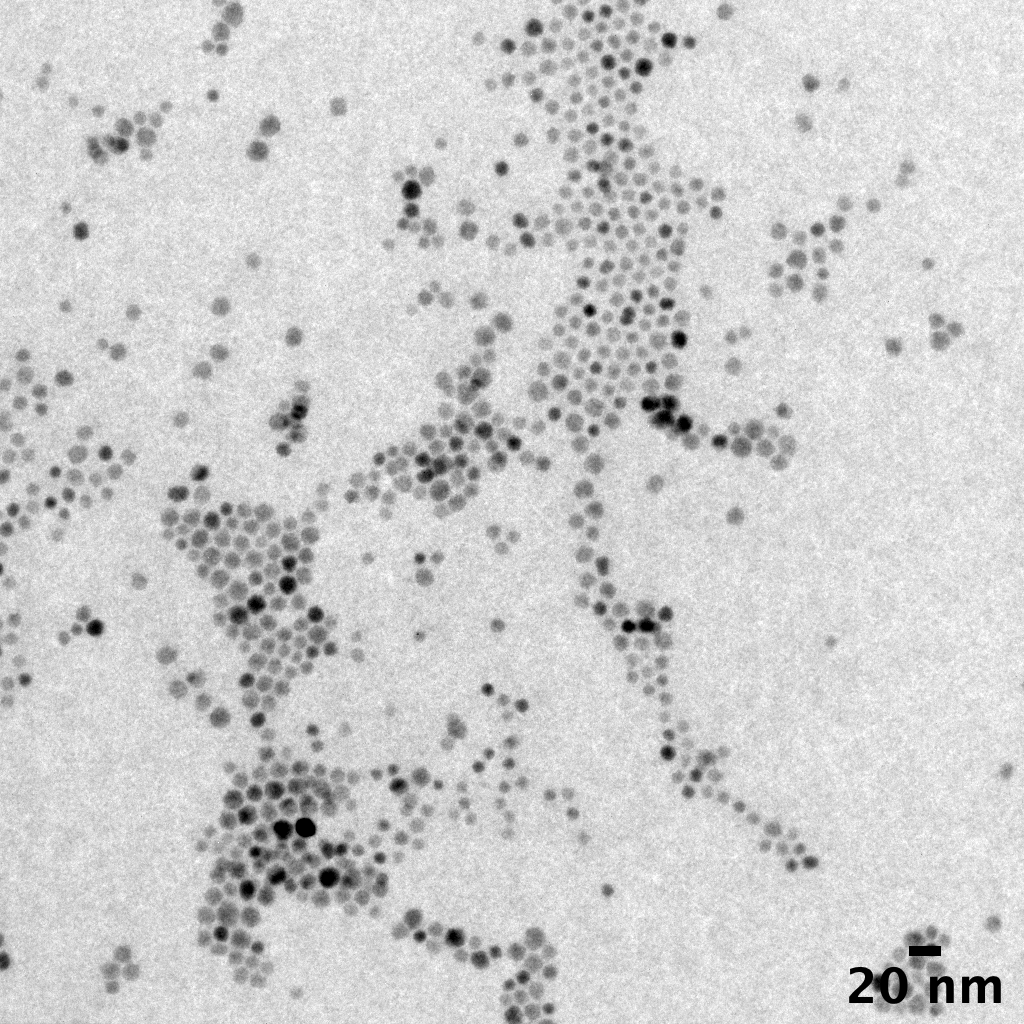
\includegraphics[width=\linewidth]{images/tem10.png}
	\end{subfigure}
	\begin{subfigure}[b]{0.3\textwidth}
		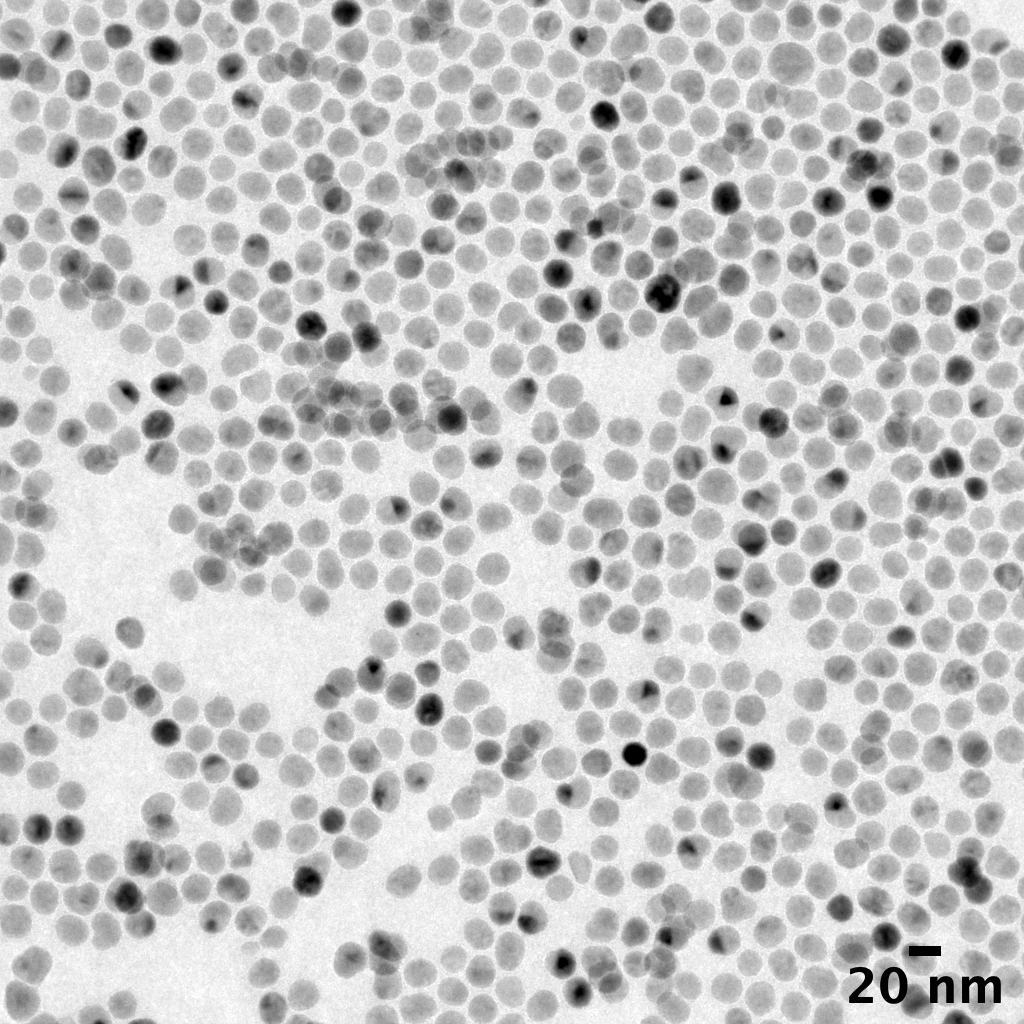
\includegraphics[width=\linewidth]{images/tem20.png}
	\end{subfigure}
\par\smallskip
	\begin{subfigure}[b]{0.3\textwidth}
		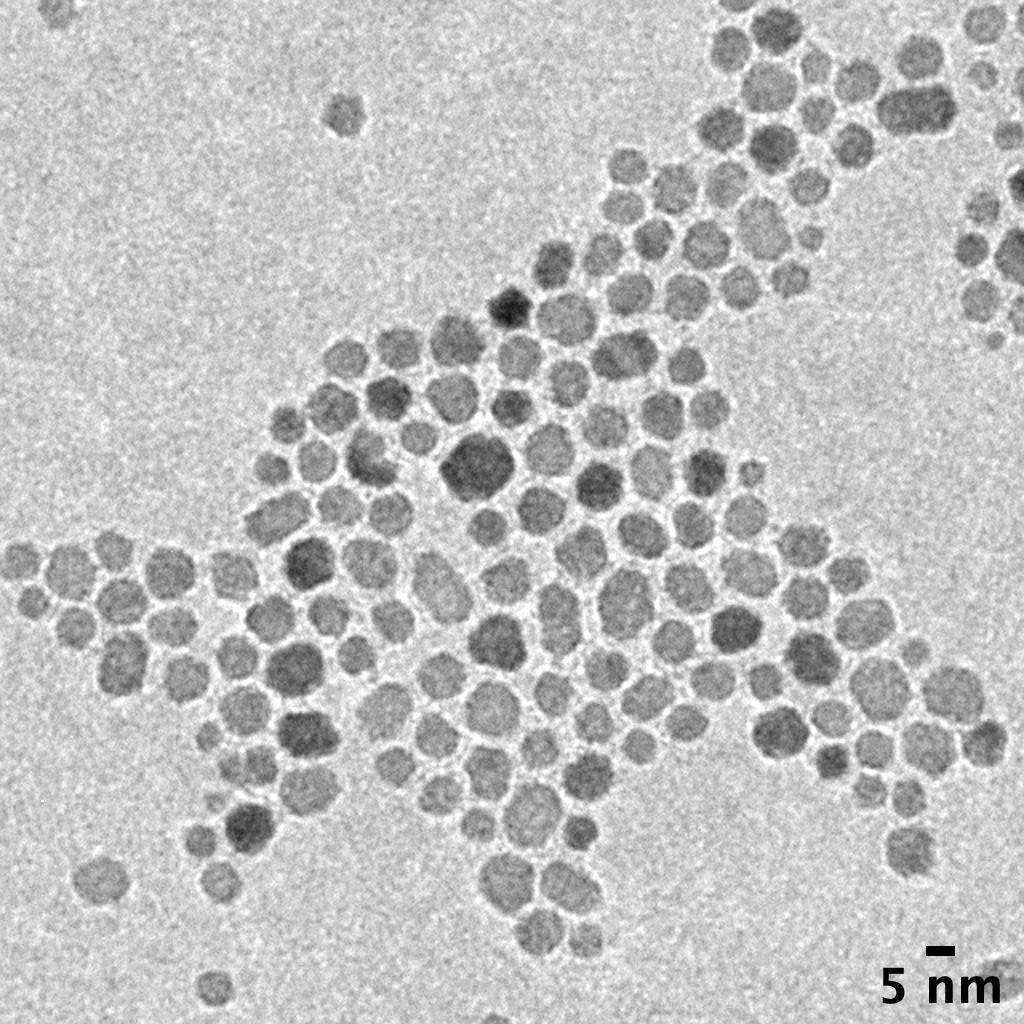
\includegraphics[width=\linewidth]{images/temh5.png}
	\end{subfigure}
	\begin{subfigure}[b]{0.3\textwidth}
		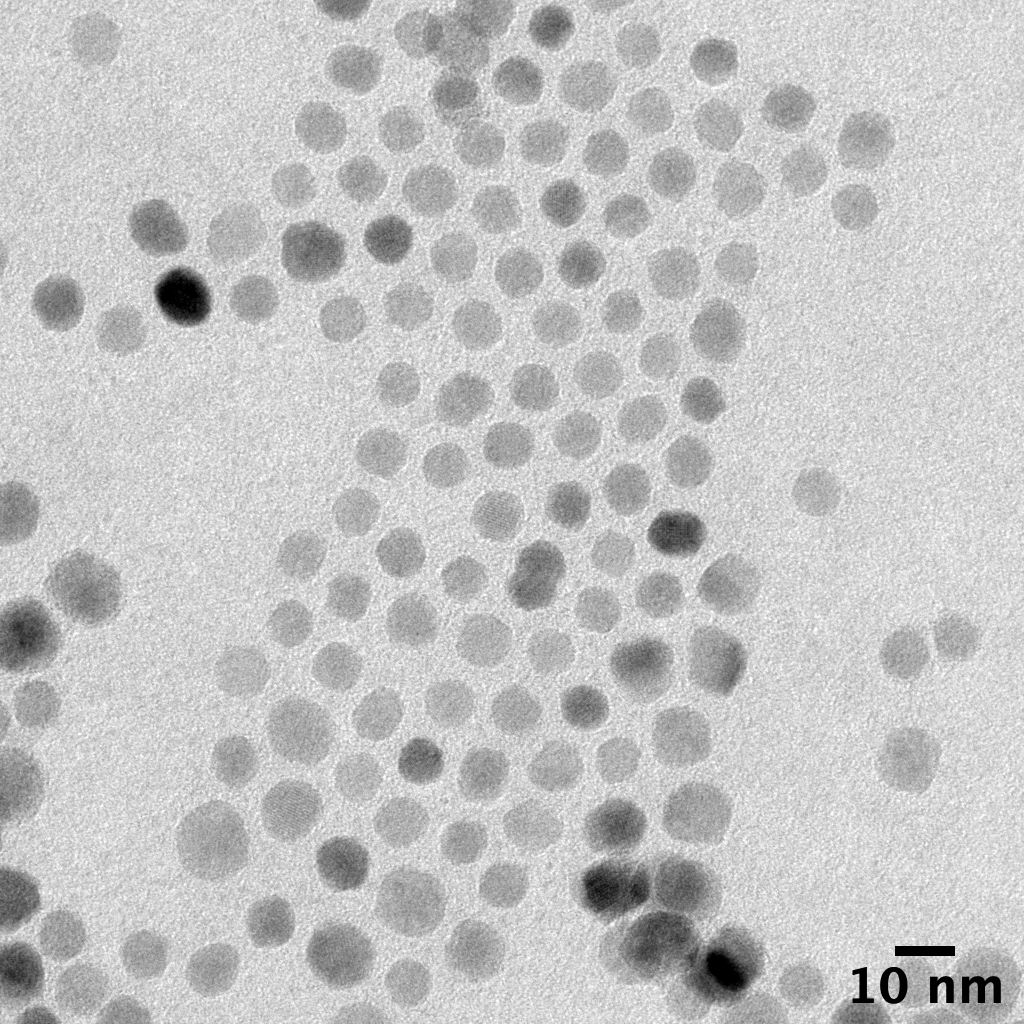
\includegraphics[width=\linewidth]{images/temh10.png}
	\end{subfigure}
	\begin{subfigure}[b]{0.3\textwidth}
		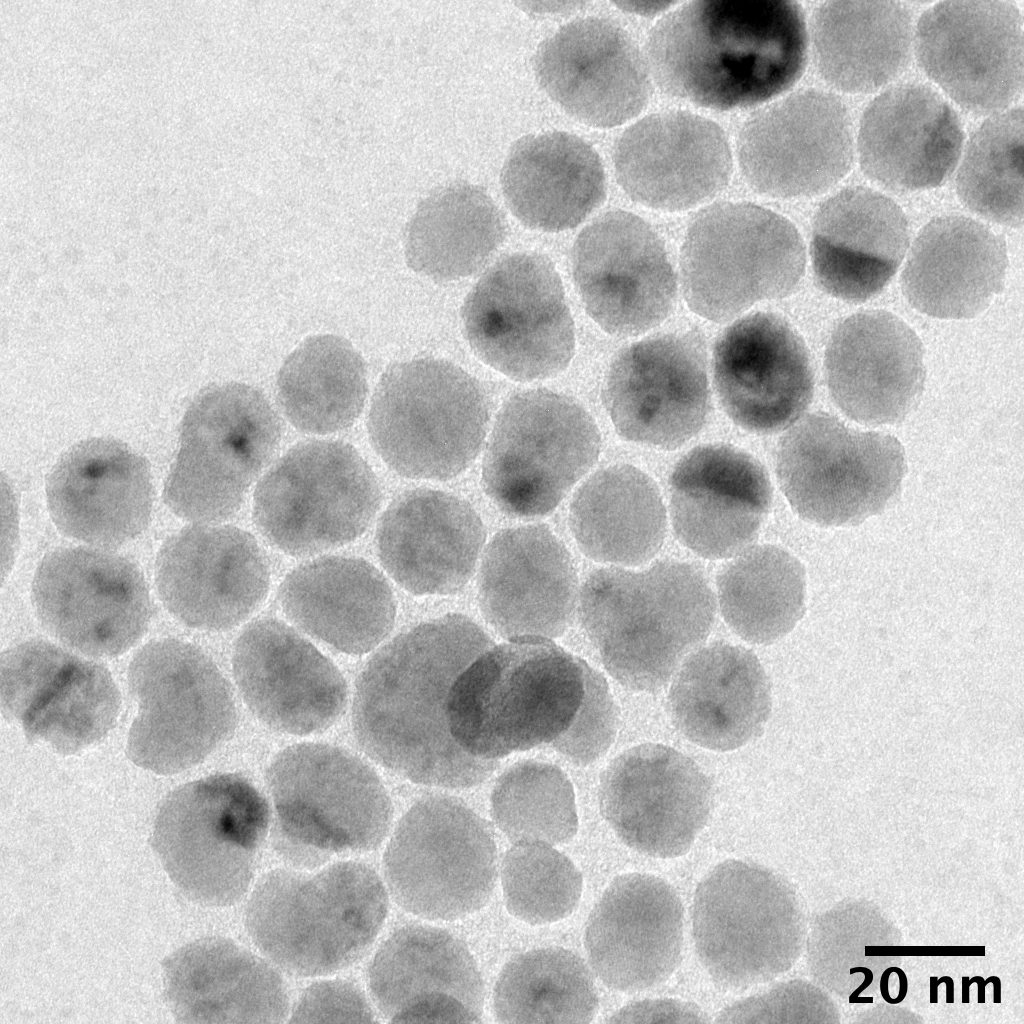
\includegraphics[width=\linewidth]{images/temh20.png}
	\end{subfigure}
\caption[TEM images of iron oxide nanoparticle]{TEM images of the iron oxide nanoparticles. From left to right: 5\,nm 10\,nm and 20\,nm nominal size in two different magnifications each (rows).}
\label{fig:tem}
\end{figure}
.


SAXS measurements of the prepared nanoparticle polymer foils where performed at the SSRL beamline 1-5. Samples were measured at 12\,keV for at two different spots for 5\,min each and averaged, a subtraction of the polymer matrix background was performed and a size distribution of spherical particles with hardsphere interaction was fitted to the radial profile. The low-q area is dominated by aggregate formation, which cannot be precisely quantified due to stray light and limited measuring range and is accounted for by a guinier-porod function, see \fref{fig:saxsps}  and  \fref{fig:saxspmma} \cite{percus1958,feigin1987,Ilavsky2009}.
The measurements do not show a clear and significant difference between the two polymer matrices. According to the regressions, the aggregates seem to have a radius of gyration of 20-30\,nm (the straylight limits the measurement validity in those small q areas), the porod $P$ of 2.5-3.8 suggests a dimensionality of the aggregates between 2 and 3.  \cite{feigin1987,lili2005}. The radii of the form factor agree within the corresponding margin of error with the values of determined by TEM measurements, the difference between the radius parameters of the structure factors and the form factor is most likely caused by the thin layer of oleic acid ligands between aggregating particles.


\begin{figure}[tp]
	\centering
	\begin{subfigure}[b]{0.3\textwidth}
		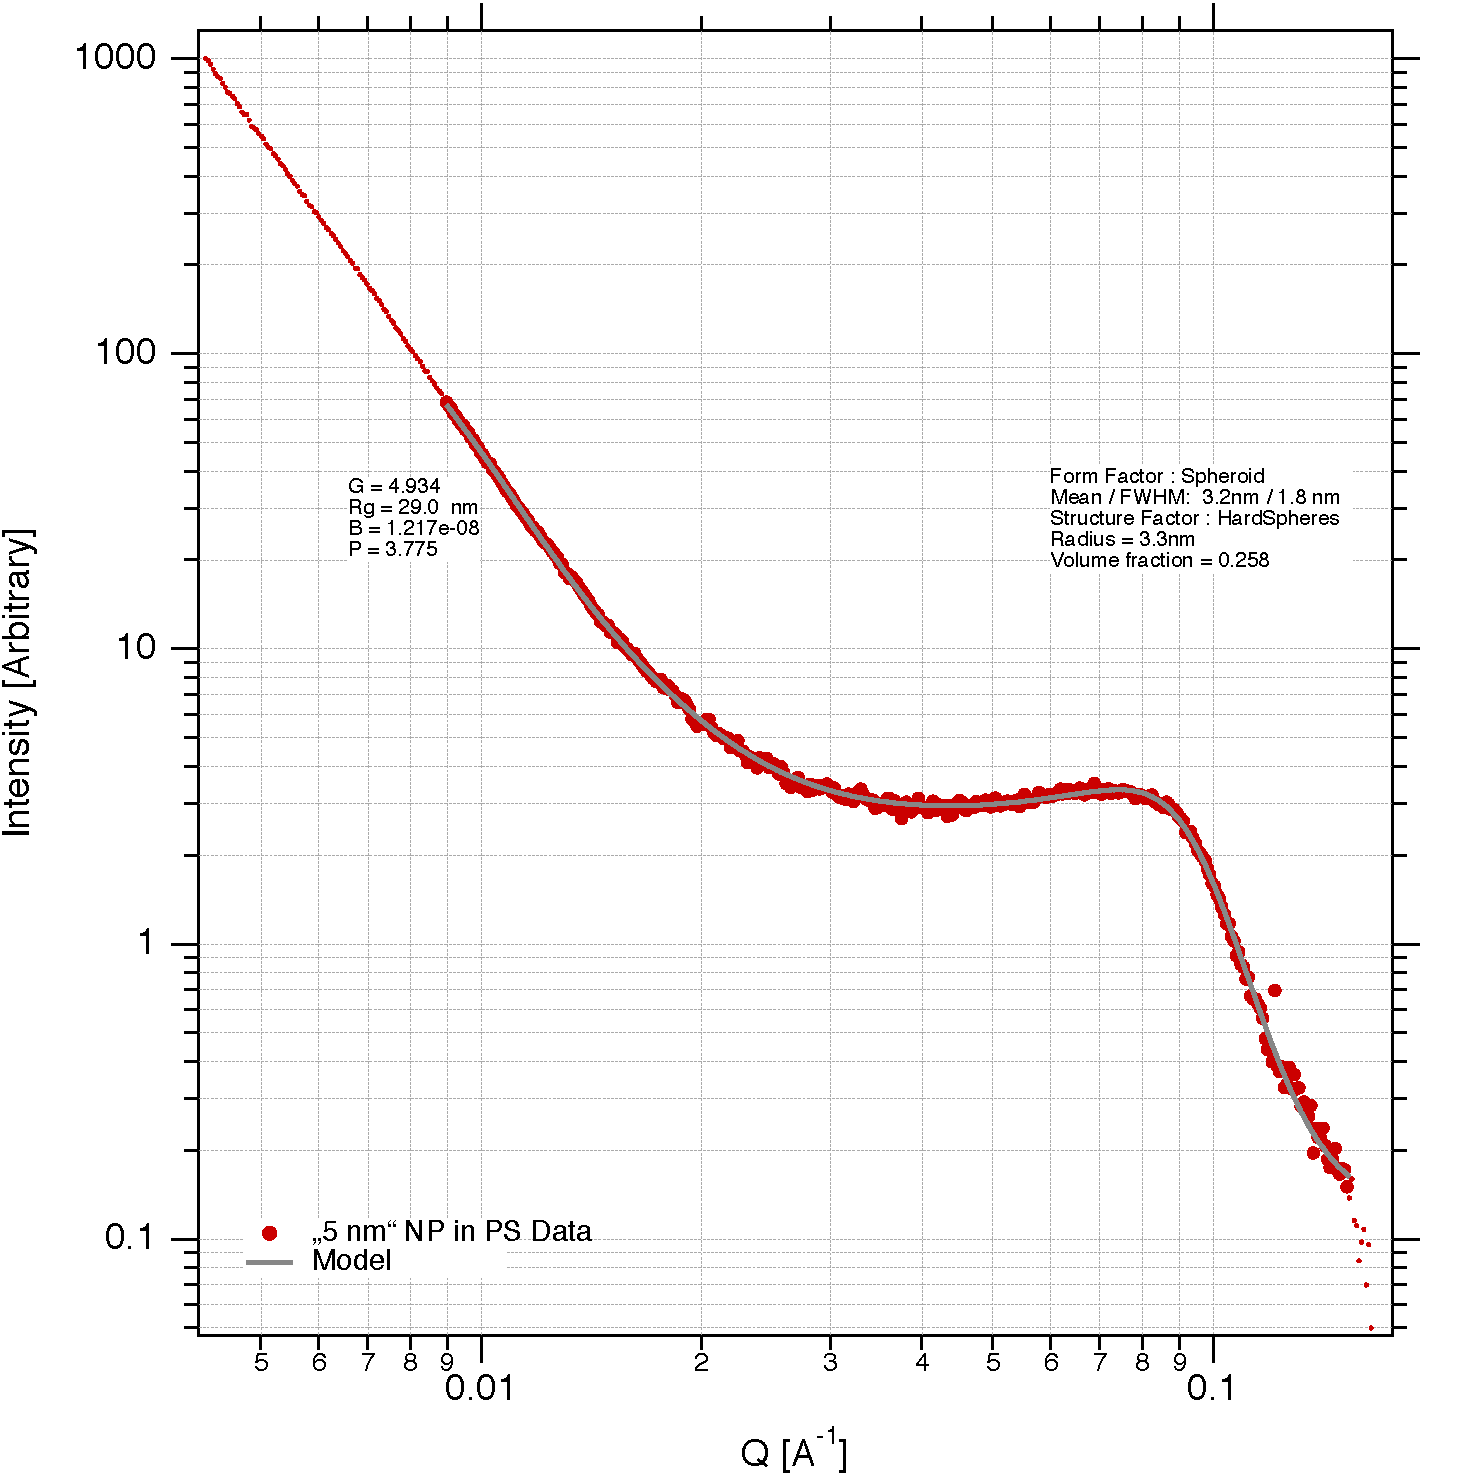
\includegraphics[width=\linewidth]{images/ps5.pdf}
	\end{subfigure}
	\begin{subfigure}[b]{0.3\textwidth}
		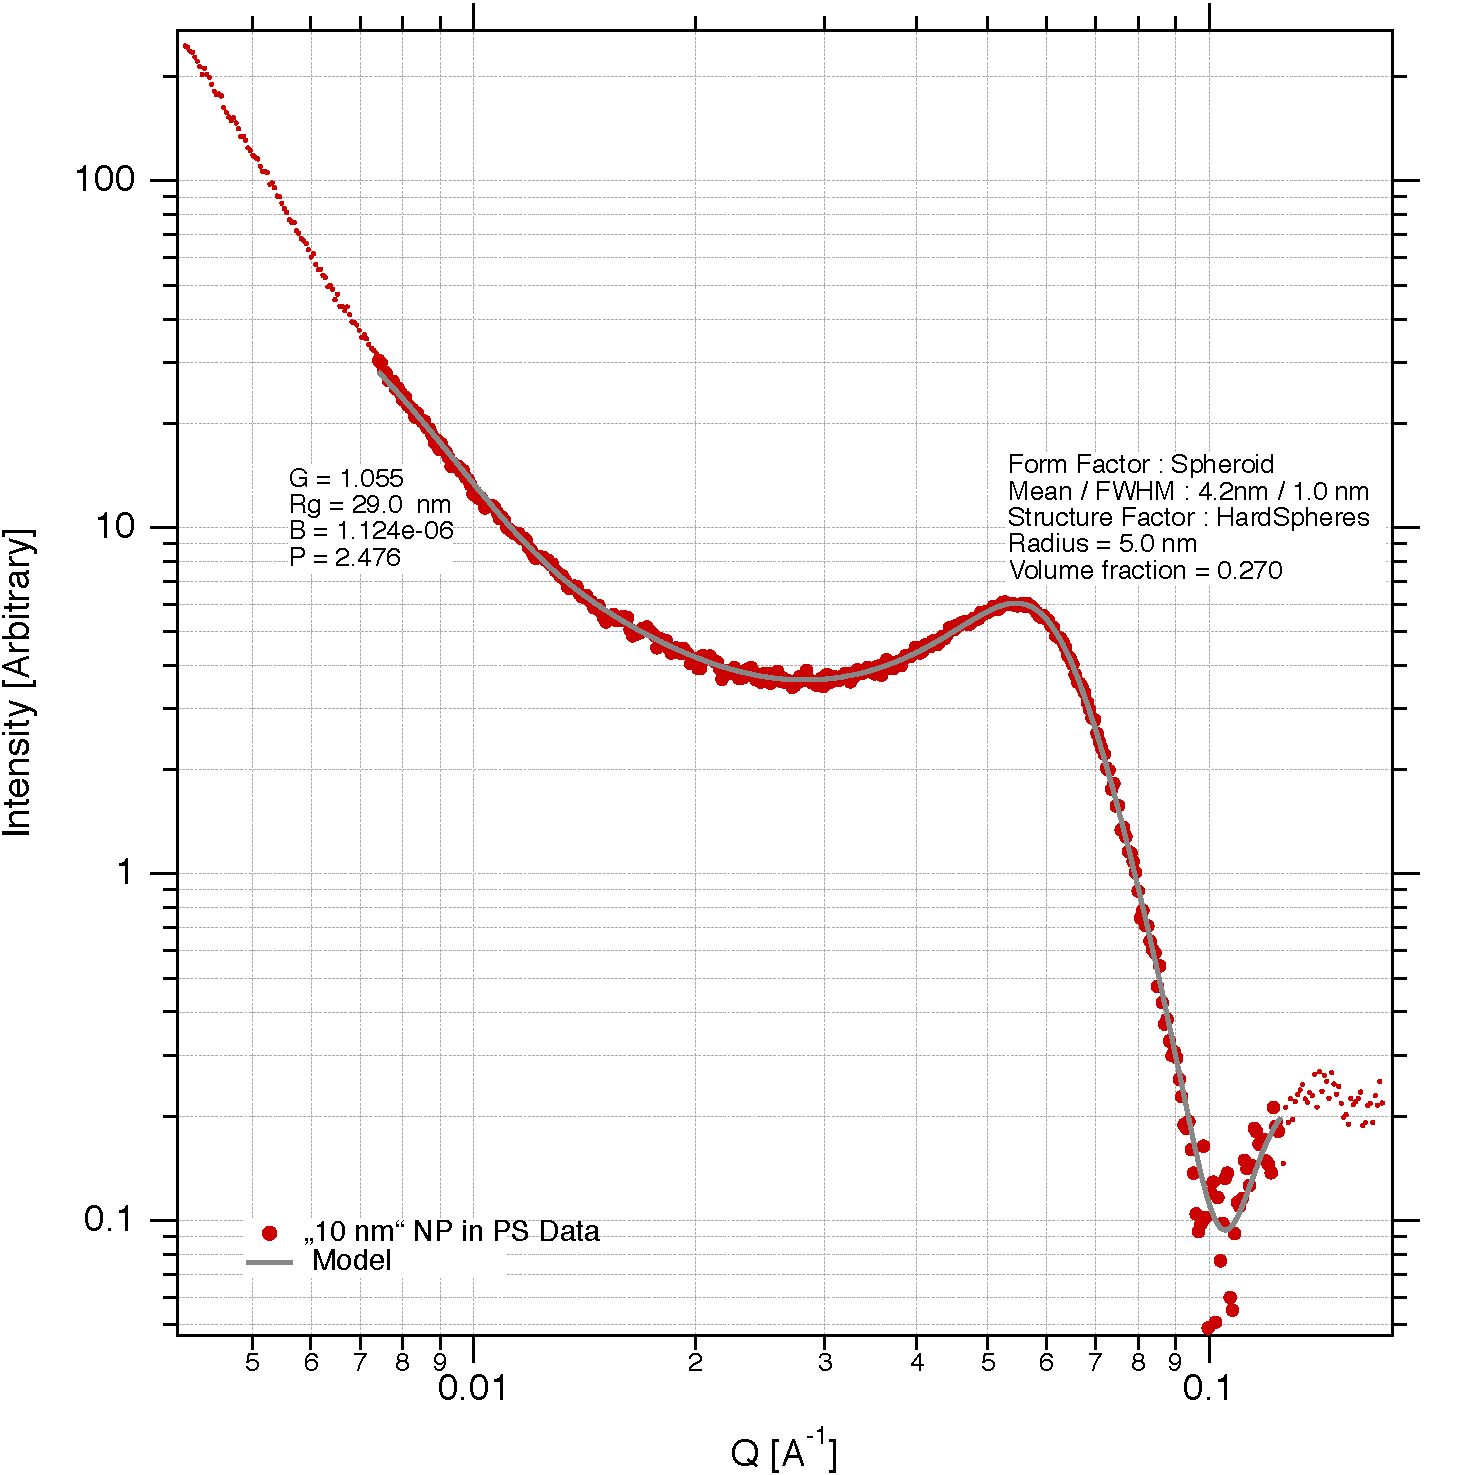
\includegraphics[width=\linewidth]{images/ps10.pdf}
	\end{subfigure}
	\begin{subfigure}[b]{0.3\textwidth}
		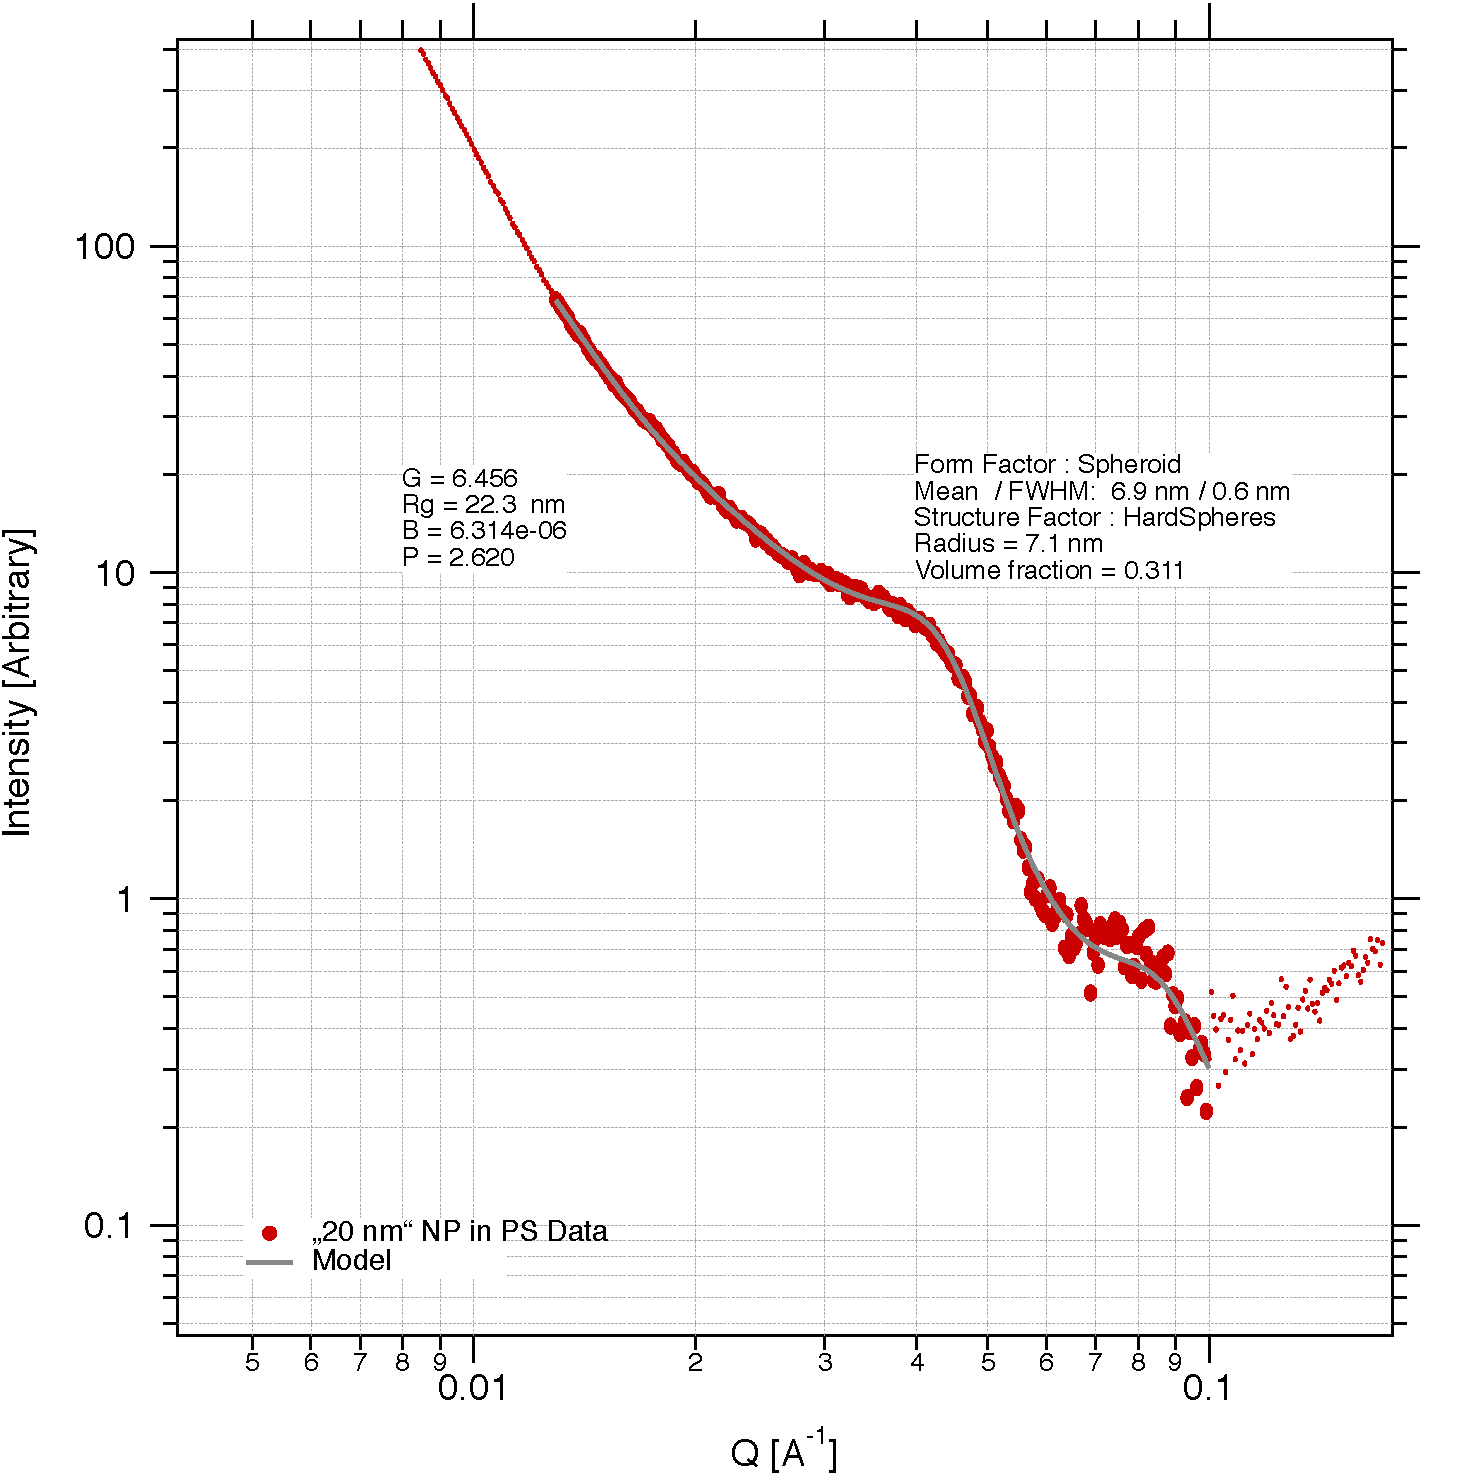
\includegraphics[width=\linewidth]{images/ps20.pdf}
	\end{subfigure}

	\caption[SAXS profile of iron oxide nanoparticles in polystyrene matrix]{SAXS profiles of nominal 5\,nm, 10\,nm and 20\,nm iron oxide nanoparticles in polystyrene matrix (left to right).}
	\label{fig:saxsps}
\end{figure}
\begin{figure}[tp]
	\centering
	\begin{subfigure}[b]{0.3\textwidth}
		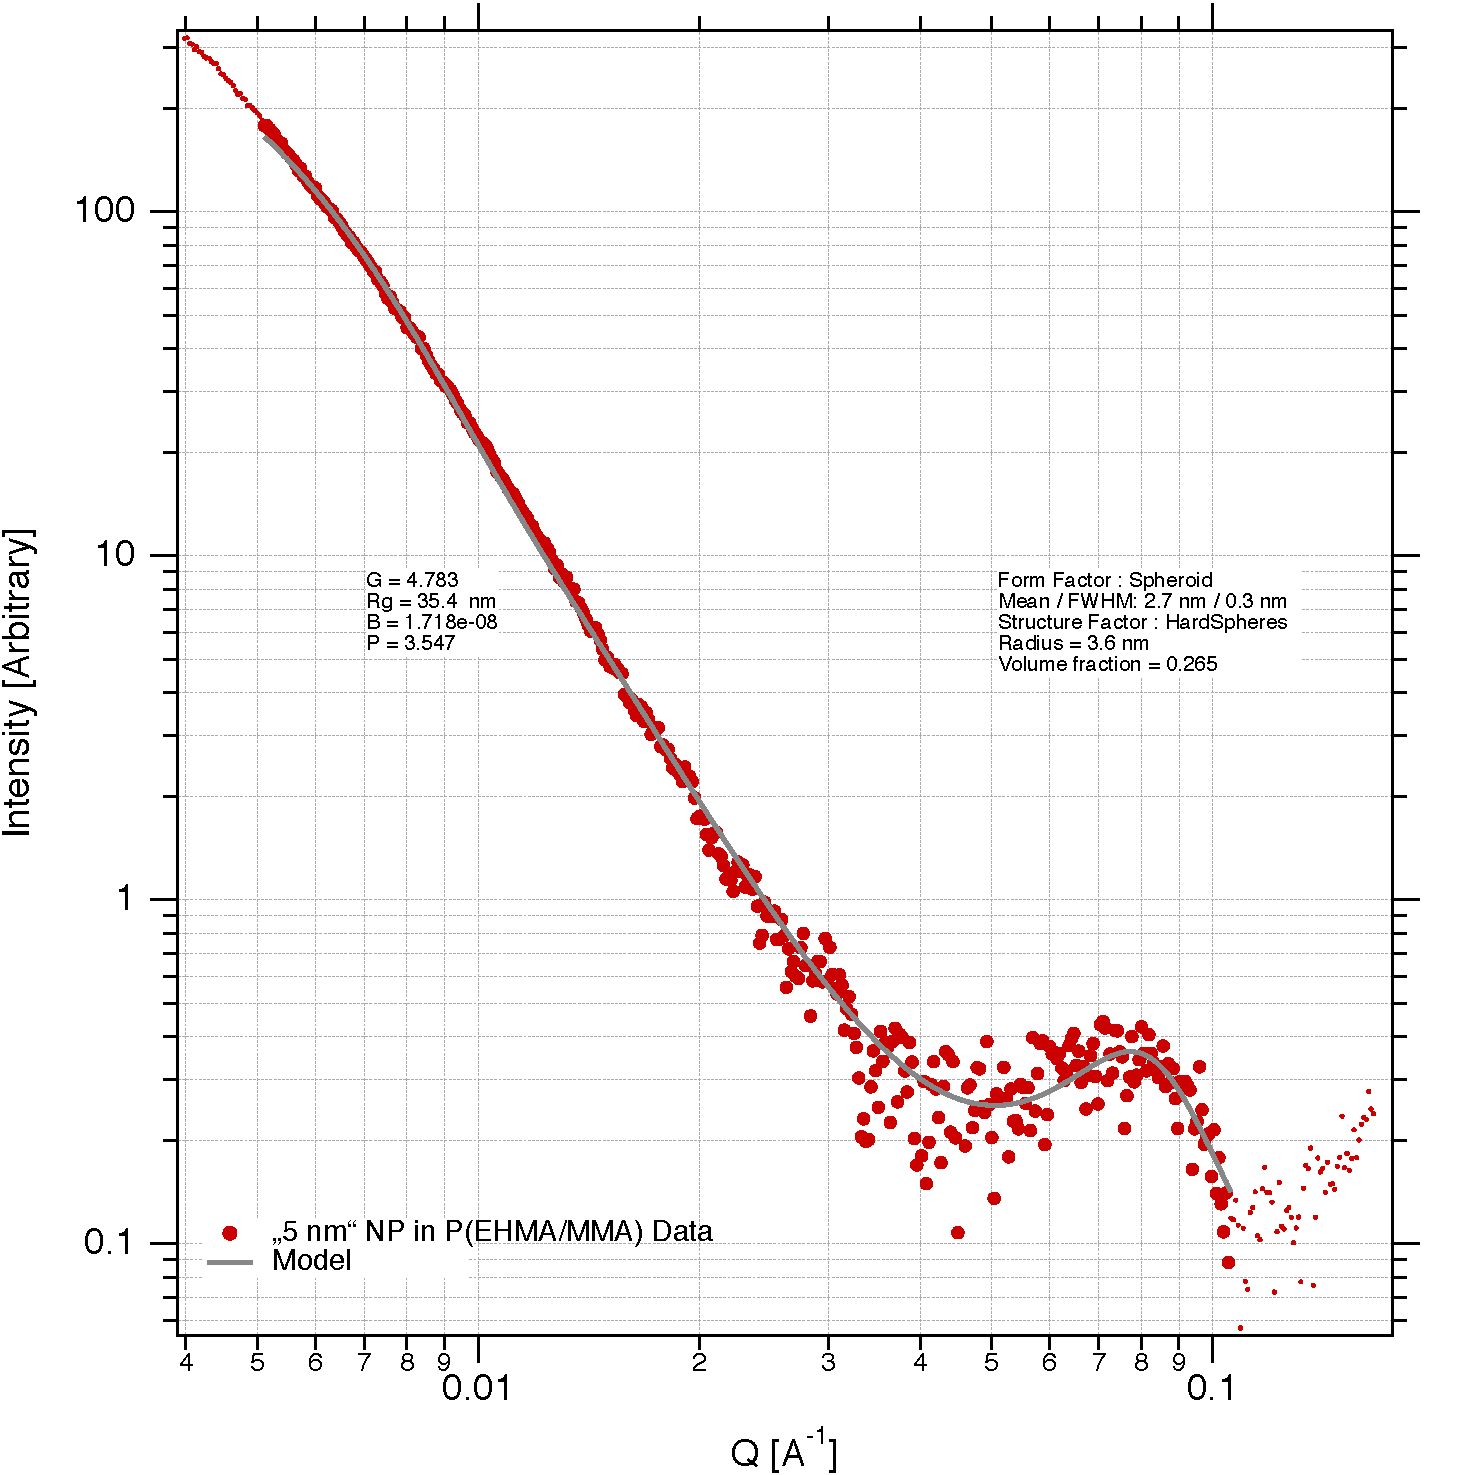
\includegraphics[width=\linewidth]{images/pmma5.pdf}
	\end{subfigure}
	\begin{subfigure}[b]{0.3\textwidth}
		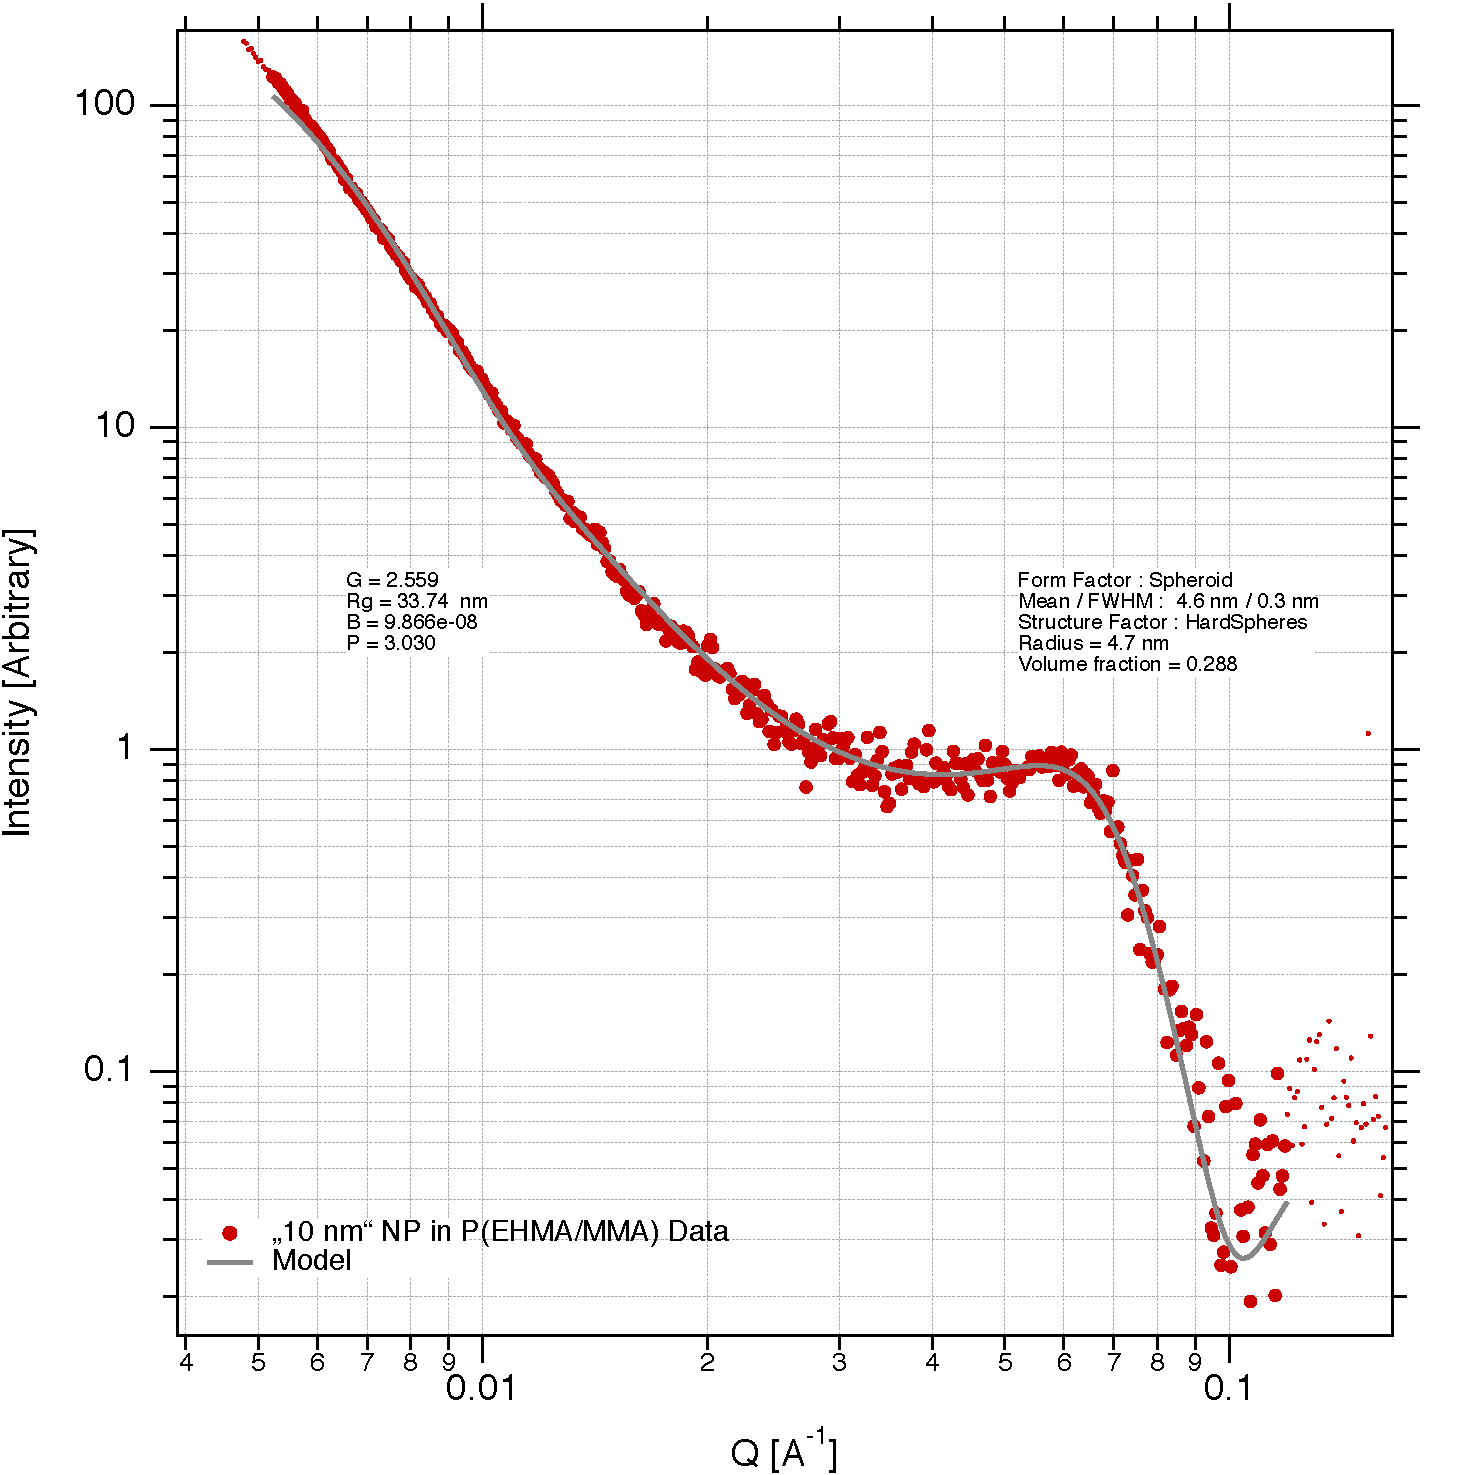
\includegraphics[width=\linewidth]{images/pmma10.pdf}
	\end{subfigure}
	\begin{subfigure}[b]{0.3\textwidth}
		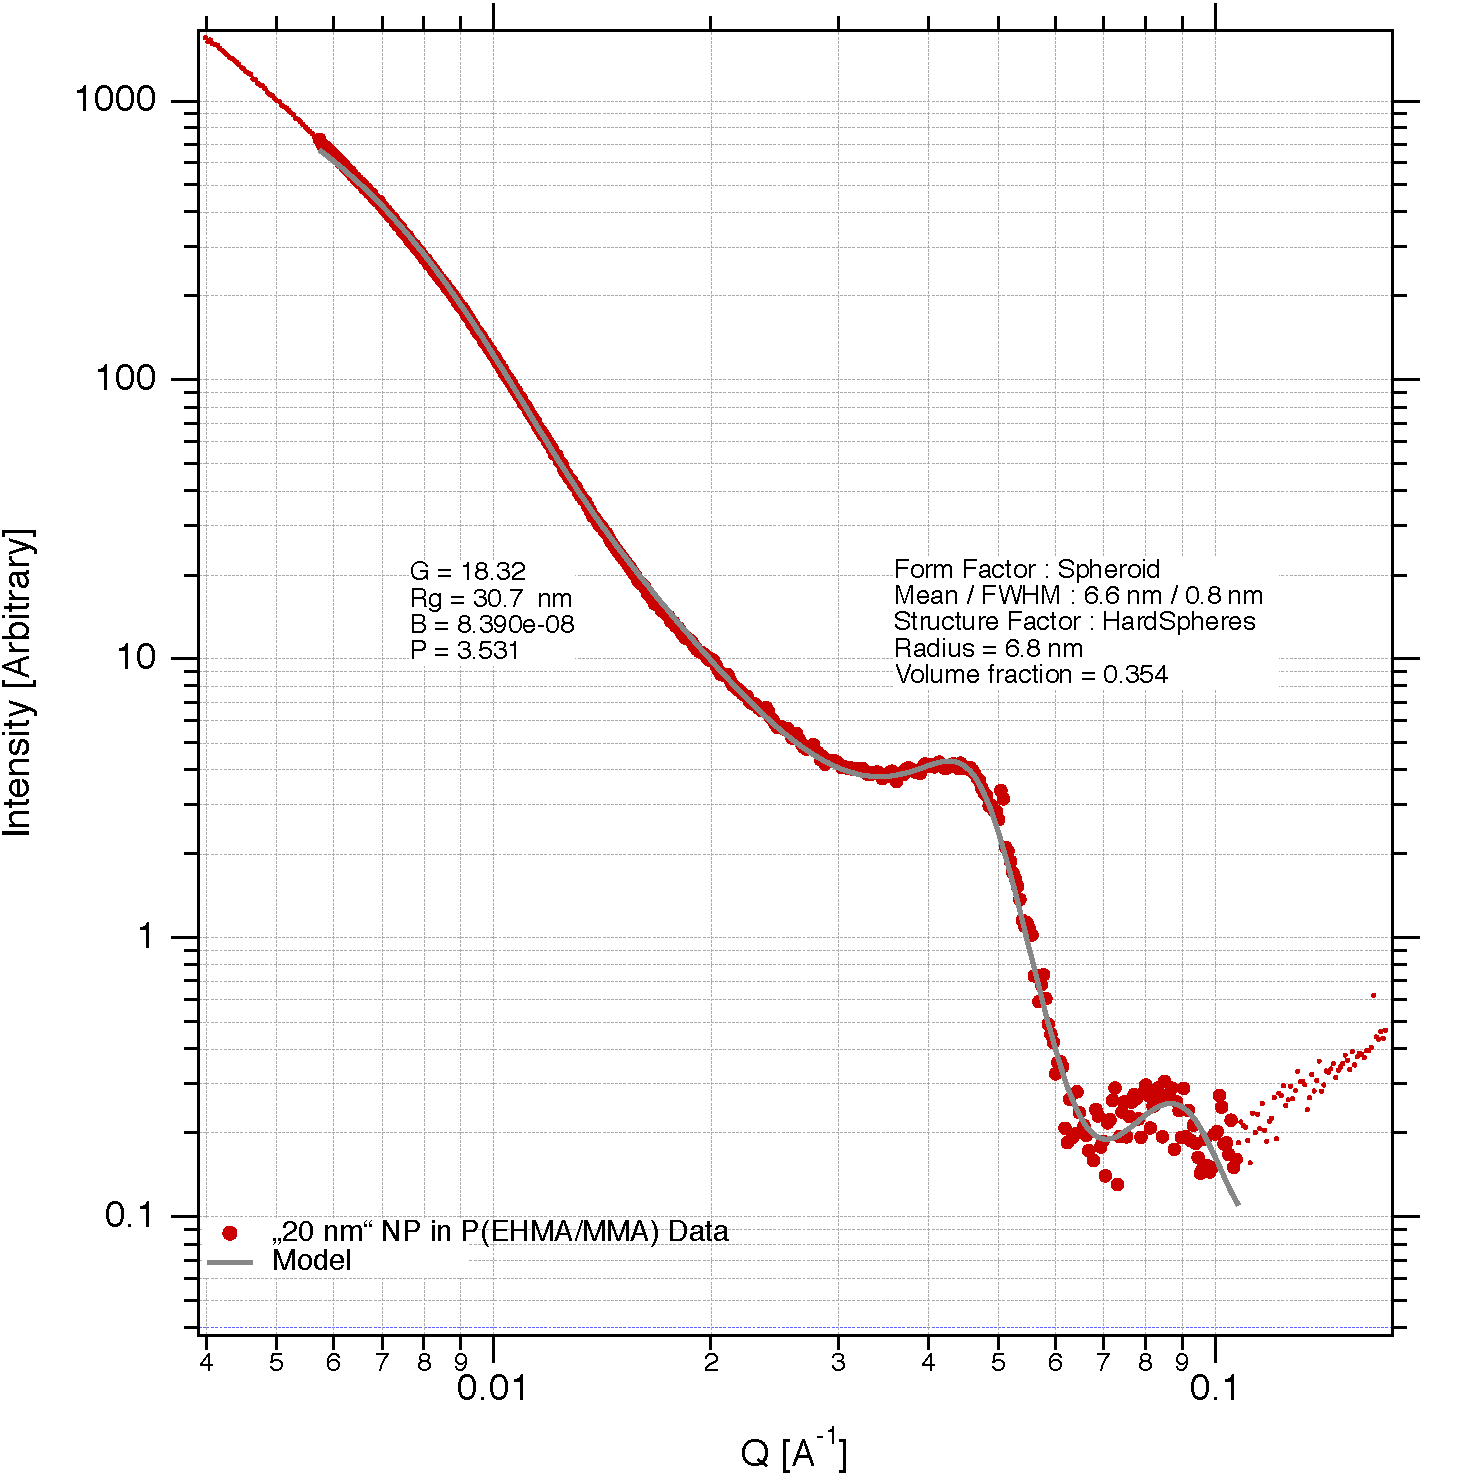
\includegraphics[width=\linewidth]{images/pmma20.pdf}
	\end{subfigure}
	
	\caption[SAXS profile of iron oxide nanoparticles in  Poly-(EHMA/MMA) matrix]{SAXS profiles of nominal 5\,nm, 10\,nm and 20\,nm iron oxide nanoparticles in Poly-(EHMA/MMA) matrix (left to right).}
	\label{fig:saxspmma}
\end{figure}

The SAXS measurements give a reasonably good insight into the expected results of the IDI scheme measurement of the same sample, which will differ due to the iron specificity and the smaller focal volume in the latter.  

\subsection{GaAs crystal films}
As a crystalline sample GaAs was chosen for its simple fcc structure and large product of the gallium K-shell fluorescence Energy and lattice constant. The samples were prepared by Ben Reeves at the Stanford Nanofabrication Facility. 
Using MOCVD, 50\,nm GaAs, 400\,nm AlGaAs as an etch stop and finally a 5\,um GaAs film were grown on an epi-ready (100)±0.1° GaAs substrate. The speciman was cut into 12\,mm\,x\,15\,mm pieces, each glued to an approx. 100\,um thick fused silica cover slip with the 5\,um film layer facing towards the silica. The substrate and the AlGaAs layer were selectively etched away via C6H8O7:H2O2 and HF:H2O wet etches, respectively. This left 5\,um thin GaAs films glued onto the the quartz slides (see \fref{fig:gaas_sample}).  XRD with Cu K-alpha was used to measure the width of the (004) GaAs bragg peak as 0.004°, indicative of high quality single crystals. 

\begin{figure}[tp]
	\centering
	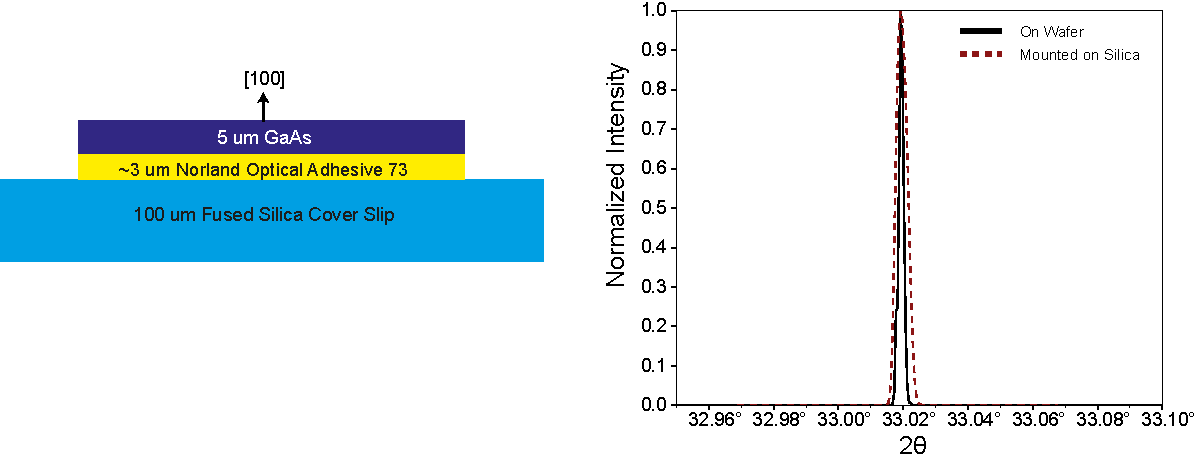
\includegraphics[width=0.8\linewidth]{images/gaas_sample.pdf}
	\caption[GaAs Sample]{Sketch of the GaAs single crystal glued to a fused silica cover slip and Cu-K$\alpha$ XRD measurement of the GaAs (004) reflex, showing a single crystal. After mounting on the cover slip, the peak is slightly broadened, most likely by an slighly uneven thickness of the glue layer. }
	\label{fig:gaas_sample}
\end{figure}


\section{Setup}
The setup used at EH5 at SACLA is shown in \fref{fig:setup}. 

The sample was mounted in an XXX angle to the beam on an XXX axis stage to allow scanning of the sample, ensure perpendicularly of the scanning directions to the beam to stay within the Rayleigh length of approx. XXX\,um while also ensuring a parallel alignment of the sample surface to one of the detectors. Overall, two MPCCD detectors were used: A Dual detector with two tiles, each 512x1024 pixels perpendicular to the FEL beam in a distance of 1\,m and a Short Working Distance Octal detector, consisting of eight 512x1024 tiles, parallel to the sample surface in a distance $d_{octal}$ ranging from XXX to XXX cm. To supress absorption and more importantly, air scattering, a vacuum pipe with Kapton windows was installed in between the sample and the Dual detector
An L-shaped aluminum plate was installed to reduce stray light as well as to allow mounting of the beamstop and filters to suppress coherent scattering and K$\beta$ fluorescence and between sample and detector.
\begin{figure}
	\centering
	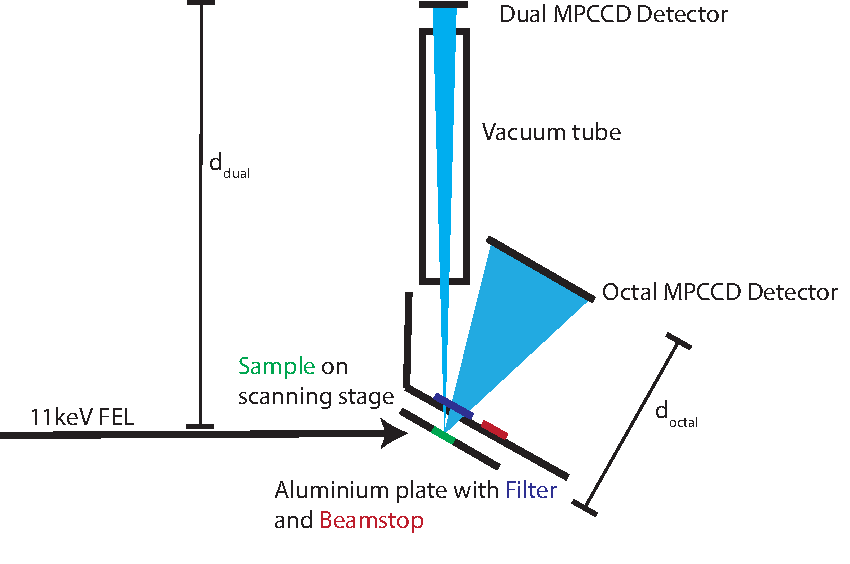
\includegraphics[width=0.8\linewidth]{images/setup.pdf}
	\caption[Experimental setup at SACLA]{Experimental setup at SACLA: The sample is mounted on a scanning stage and aligned to stay in focus during the scan and be parallel to the Octal MPCCD detector, which is in a distance $d_{octal}$. The angle between incoming FEL and Sample is XXX. Behind the sample, a stray light filter, beamstop and (depending on the sample) a filter foil is installed. The Dual detector is mounted $d_{dual}$=1\,m away from the sample in a XXX angle. To reduce air scattering, a vacuum tube is installed in the path from sample to Dual.}
	\label{fig:setup}
\end{figure}
\paragraph{Imaging the Focus}
The image to focus, 
\paragraph{Imaging Nanoparticles}
\paragraph{Imaging Crystals}

\section{Data Processing}
As the amount of recorded data is huge, an efficient strategy for filtering on shots, preprocessing the data to eliminate interferences and finally reconstruction has to be implemented.
\subsection{Shot filtering}
\subsection{Preprocessing}



\begin{figure}[tp]
	\centering
	\begin{subfigure}[b]{0.45\textwidth}
		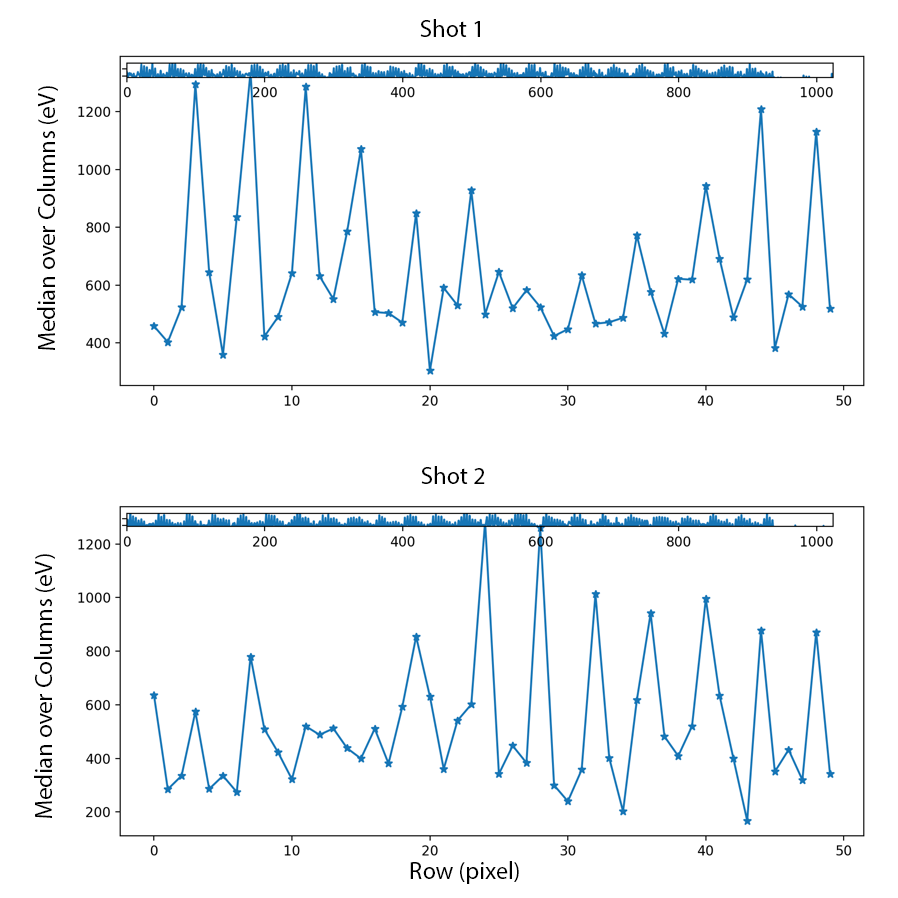
\includegraphics[width=\linewidth]{images/octalissue2.png}
	\end{subfigure}
	\begin{subfigure}[b]{0.45\textwidth}
		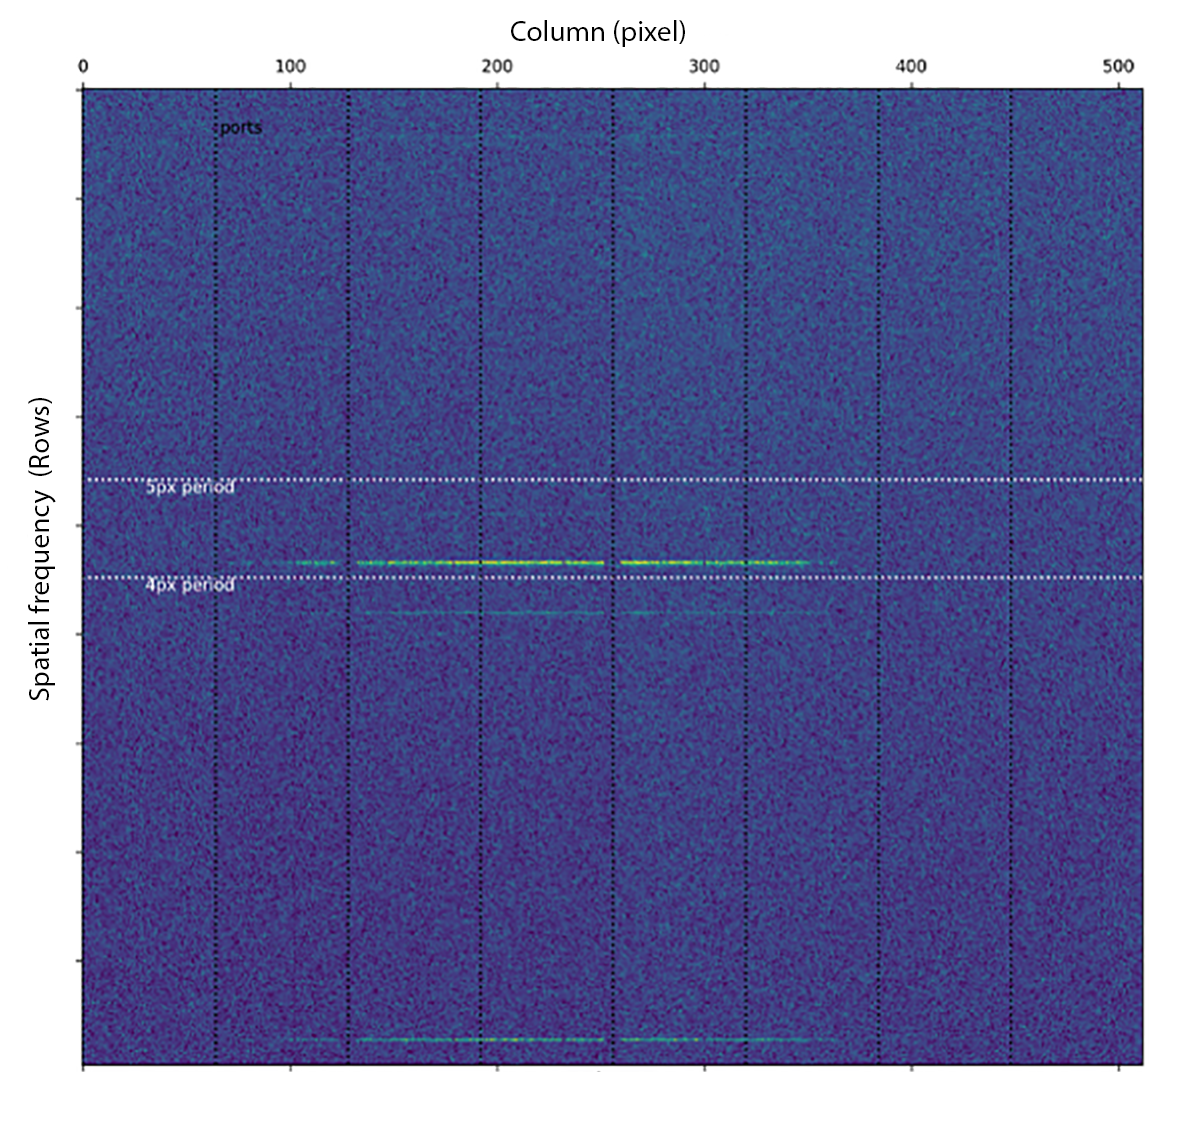
\includegraphics[width=\linewidth]{images/octalissue.png}
	\end{subfigure}

	\caption[Periodic noise on octal detector]{Periodic noise on octal detector after background subtraction: For two exemplary shots the median over columns of one detector tile is shown. A periodic noise is visible. The mean spatial spectrum (over the rows) for each column of the tile is shown on the right. The periodic noise is not uniformly affecting all the columns of the tile.}
	\label{fig:octalissue}
\end{figure}



\begin{figure}
	\centering
	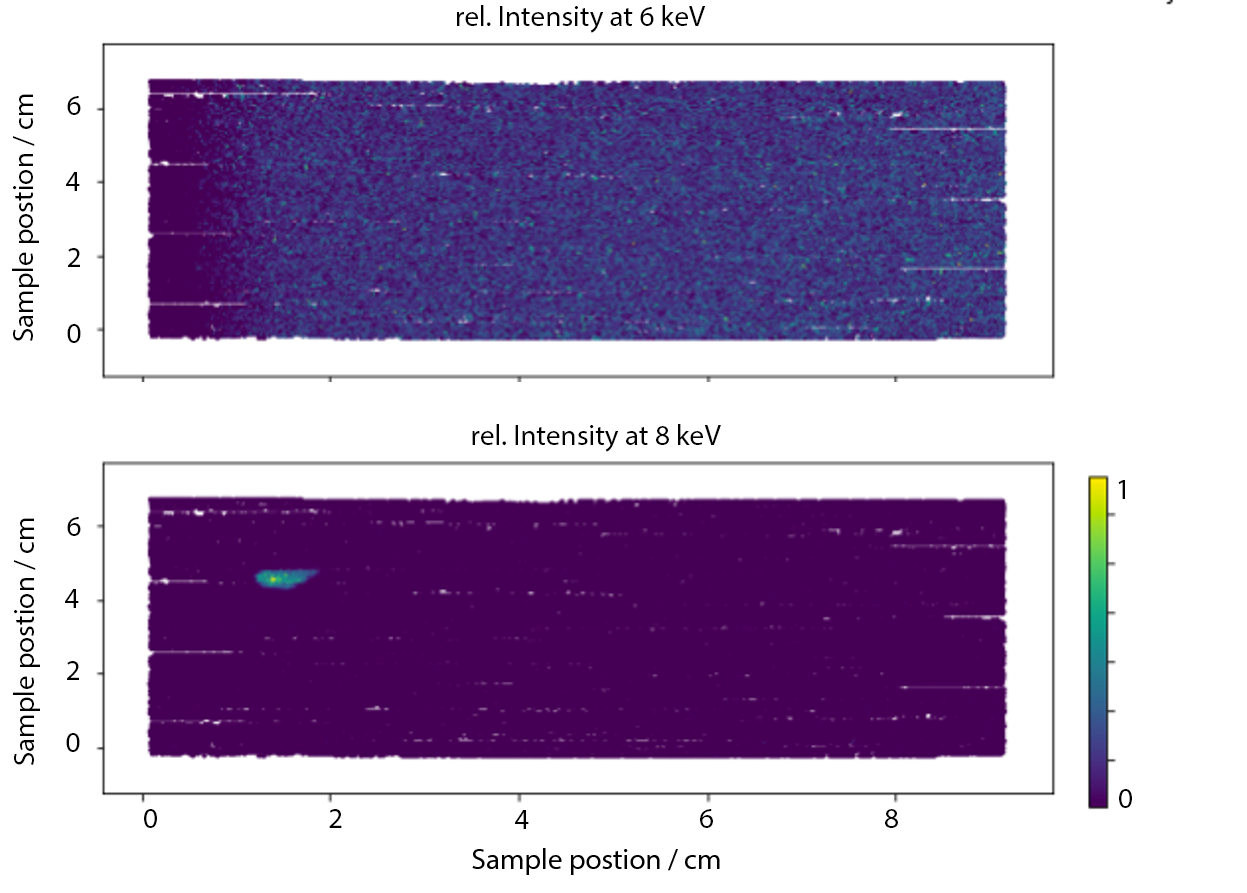
\includegraphics[width=0.9\linewidth]{images/xrf.png}
	\caption[Exemplary relative intensity of the 6 keV and 8 keV photon peak on the detector for different scanning positions on the sample]{Exemplary relative intensity of the 6 keV and 8 keV photon peak on the detector for different scanning positions on the sample. In this iron sample, a localized impurity, most likely copper, is clearly visible and can be masked out .}
\end{figure}

\begin{figure}
	\centering
	\begin{subfigure}{0.45\textwidth}
		
\includegraphics[width=\linewidth]{images/mask.png}
	\end{subfigure}
	\begin{subfigure}{0.45\textwidth}
		
\includegraphics[width=\linewidth]{images/mask.png}
	\end{subfigure}
	\caption[Usable detector area]{Usable detector area (yellow) of the dual (a) and octal (b) detector after signal correction and statistical filtering. Only the intersection of good areas for each run will be used. This way the same mask and number of correlation pairs will be used for samples that will be compared to each other.}	
\end{figure}

\paragraph{Shot filtering}

\paragraph{Filtering by sample position}
\paragraph{Detector masking}

\paragraph{Photon counting}



As shown in \fref{fig:spectrum}, the background corrected and masked spectrum of the detector shows peaks at multiplex of the fluorescence and excitation energy with a FWHM of .... . 


As discussed in \fref{chap:simulation}, the number of fluorescence photons can be estimated...


% Raw Data
% Spectrum
% Peaks


\paragraph{Crystal orientation}
For determining the relative orientation of the crystal with regards to the detector, Kossel lines as described in \fref{chap:kossel} can be used.  A semi-automatic alignment program was developed (\fref{fig:kosselfit}) and used the find the crystal orientation (\fref{tab:kosselfit}). As initial parameters, 5.65\,\AA\, lattice constant, 9.25\,keV energy and 800\,px detector distance and the result of a simple 2D cubic fit for the values of the translational shift were used. 
\begin{figure}
	\centering
	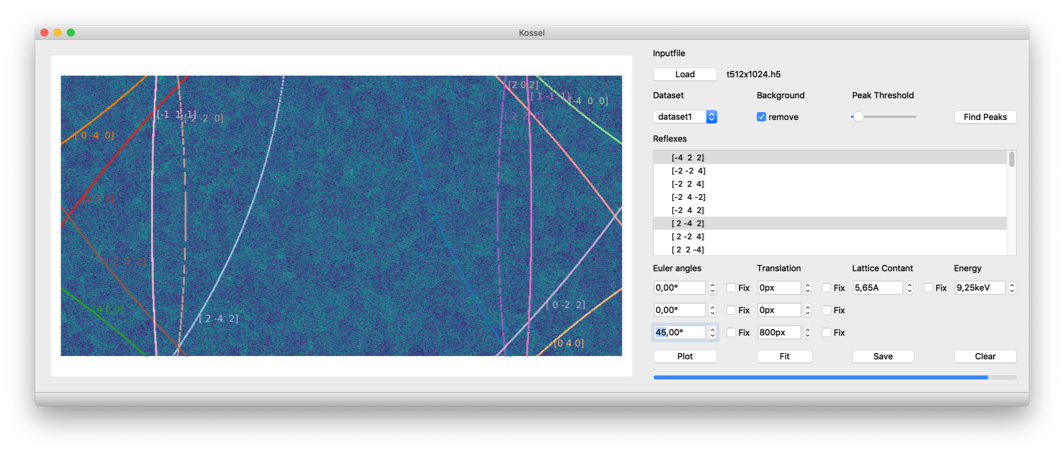
\includegraphics[width=0.8\linewidth]{images/kosselfit.png}
	\caption{Program for fitting Kossel lines to experimental data}
	\label{fig:kosselfit}
\end{figure}

\subsection{Reconstruction}




\section{Results}
\subsection{Imaging the Focus}
\subsubsection{Filtering}

\subsection{Imaging Nanoparticles}
\subsubsection{Filtering}
\subsection{Imaging Crystals}



\begin{table}[]
	\caption{Results of the Kossel line analysis}
	\begin{tabular}{lllll}
		\hline
		Sample & Initial Translation & Initial Rotation    & Energy & Rotation           \\
		& x,y in pixels      & Euler angles x,y,z & in keV    & Euler angles x,y,z \\
		\hline
		GaAs 1 &                    &                    &        &                    \\
		GaAs 2 &                    &                    &        &                   \\
		\hline
	\end{tabular}

\label{tab:kosselfit}
\end{table}

\section{Discussion}
The estimated number of overlaid modes from the foil spectra is lower than expected. However, one must keep in mind that the used regression scheme has a low sensitivity for higher $M$ values due to the diminishing gradient and might underestimate the number of modes. Nevertheless, this indicates that the number of modes is much higher than the \enquote{optimal} value for unpolarized light ($M=2$), resulting in severely reduced contrast. 
As the measurement was performed perpendicular the the FEL beam coherent scattering was many orders of magnitude weaker than the fluorescence.  Therefore, in contrast to previous experiments, any observed intensity correlations can only stem from the incoherent fluorescence.
The disappearance of the observed correlations after defocusing strongly suggests that they actually include spatial information about the sample and are not caused by detector artifacts. This could be further examined in future experiments by simply rotating the detector and observing if the reconstruction rotates as well. The amplitude observed in the foil samples matches approximately the result of the simulation presented in \fref{chap:simulation}  (\fref{fig:simfoil}) after accounting for polarization and multiple emission lines but is a factor of 2-4 less than previously measured by Inoue et al. and suggests more than 200 modes \cite{inoue2019}. At its root, there might be various causes for this: 1) a longer pulse length as a result of the less strict filtering of the shots (a different trade-off chosen with regards to peak contrast vs. noise reduction by averaging over more images), 2) the only partially by the regression corrected undersampling and 3) the higher observation angle creating additional spatial modes. For an accurate measurement of the focal width in horizontal and vertical direction, the experiment would have had to be conducted in a small angle regime with the foil placed perpendicular to the beam and the detector placed close to forward direction. 

The nanoparticle samples have much less prominent features according to the SAXS measurements than initially planned and compared to the structure factor for non-interacting spheres, leading to an overestimated SNR in the simulations. The SAXS measurements give a reasonably good insight into the expected results of the IDI measurement of the same sample. However, there will be some differences in the reconstructed structure factor due to the iron specificity of IDI and the smaller focal volume capturing fewer aggregates. Mechanical limitations in the experimental setup made is necessary to perform the experiment with the excitation beam under a 45° angle. The path length differences due to this angle and the relatively high thickness of the samples created a large number spatio-temporal modes reducing the contrast. At the time of sample simulations, design, and preparation, this experimental limitation was not yet known and therefore not considered.
Optimization of the preparation method resulting either in higher concentrations of non-aggregating particles or to complete aggregation and the formation of super-crystals might lead to stronger features. Also, liquid injectors might be an option, even if there would be clear practical downsides: The tight focus and short Rayleigh length would make it difficult to achieve spatial overlap of the beam and sample and controlling the number of particles in the focal volume would be challenging. Taken together, the results indicate that follow-up measurements should be designed to be in forward direction under the small-angle regime to reduce the detrimental effect of the sample thickness.

The achieved alignment of the crystalline samples after determination of the mean orientation and translational offset is still worse than the resolution of the reconstruction and the size of the expected Bragg peaks. This results most likely in a reduction of the signal contrast through averaging of different pixel pairs not belonging to the same true $\vec{q}$. Mounting of the sample and the damage done during the measurement by the focused beam might have resulted in a slight bending of the thin glass stabilizing the crystal sheet. The resulting variations of the orientation over the scanning of the sample would not have been corrected, as the alignment has only been performed on averaged images.  Furthermore, it has proved to be challenging to validate that the orientation correction works as designed and the Bragg peaks would be reconstructed at the positions chosen as regions-of-interest. A non-comprehensive search using local maxima filter (as used to determine the Bragg peak positions in the simulated correlations for \fref{fig:accesiblebraggq}) did not lead to reasonable, i.e., symmetric and at the correct $\left|\vec{q}\right|$, candidates at other positions.
The energy of the excitation X-ray being close to the gallium K$_\alpha$ energy to avoid excitation of the arsenic atoms makes it impossible to quantify or filter coherent scattering in the recorded data. Combined, it is concealable that these effects reduced the peak intensity below the noise level. 

Severe detector artifacts unnoticed during the experiment reduced the amount of usable data significantly -- showing the necessity of better continuous online monitoring of the recorded data. The photon-counting applied to the raw images improved the fidelity of the focal images. Depending on the PSF of the detectors and sufficiently low photon counts, more sophisticated droplet schemes based on error minimization while incorporating the scattering photon and allowing for subpixel resolution, or using a neural network trained on synthetic images could further reduce the influence of noise and undersampling and might increase the contrast in for the single crystal images \cite{baumann2018,collaboration2014,schayck2020,sun2020}.\\
Even though the application of non-uniform FFT (NUFFT) based correlation estimators with sophisticated interpolation kernels, which have successfully been used in other fields, would require more memory, the reduction in under-sampling by making full use of the smaller $\vec{q}$ spacing at higher detector angles could make it a worthwhile extension of the used 3D reconstruction \cite{laguna1998,yang2008,chang2020}. Another possible avenue for improvement of the implementation might be to reconstruct only relevant parts of the reciprocal space, significantly reducing computational time and memory requirements. 


\chapter{Conclusion and Outlook}

\section{Developed tools for CDI/IDI experiments}
Both the GPU-accelerated simulation code and the reconstruction code developed for this thesis are open source\footnote{available under \url{https;//github.com/fzimmermann89/idi}} and will be used for planning and analyzing future IDI experiments. The simulation code allows to compare IDI and CDI experiments for the same sample, comparison for different samples and experimental parameters as shown in \fref{chap:simulation}.
The analysis code implements 2d, 3d and radial correlations for small and wide angle experiments with different normalization approaches as well as library of commonly needed auxiliary functions, such as dark and mask generation for pixel detectors, a new common mode correction with adaptive block sizes, photon counting procedures, different regression tools as well as tools for center finding and similar tasks.
Furthermore, the Kossel line alignment tool with its graphical user interface allows easy analysis of the detector orientation for future experiments with strict alignment margins.


\section{Using Incoherent Imaging for Online Beam Diagnostic}



The posibility to run an IDI setup in parallel with other detectors would allow for a combination of IDI with CDI

Larger detectors

Short pulses

Element specific 


Even just the ability to image to focal volume might be an useful diagnostic tool in certain experiments




\begin{figure}
	\centering
	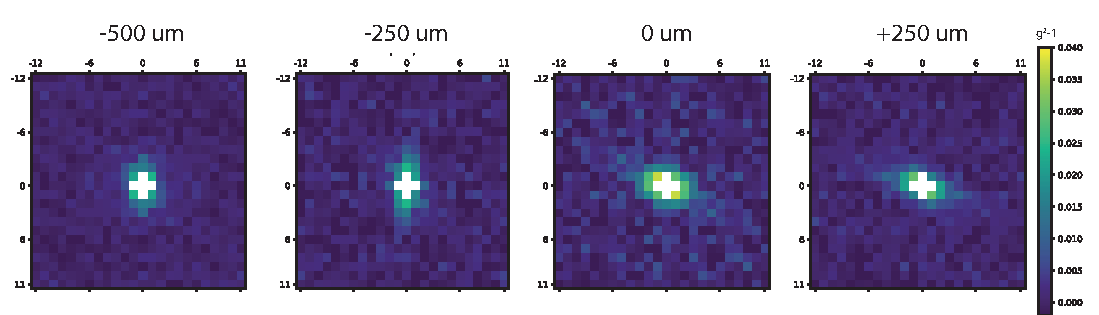
\includegraphics[width=\linewidth]{images/lv65_vanadium.pdf}
	\label{fig:outlook_vanadium}
	\caption[Focus finding using IDI]{Preliminary results of the $g^2(\vec{q})$ calculation of the fluorescence of a 4\,um vanadium foil, placed at 4 different positions along the x-ray beam at the CXI experimental hutch (LCLS, running in an experimental configuration for short pulse duration under 1\,fs \cite{subfs2017,argosecond}) using the "100 nm" KB focusing (optimal theoretical focus size 90\,nm x 150\,nm, theoretical beam divergence 2 mrad x 1 mrad) on one tile of a Jungfrau detector (75\,um pixelsize, placed 480\,mm downstream of the sample). The axis are in detector pixels. Shown are averages over ~2000 shots with minimal shot based filtering. The position captioned "0" was determined during the experiment as the focus based on these results, the other positions are 250\,um and 500\,um further downstream and 250\,um upstream (this position was previously determined as the focus by imprints).  Some astigmatism is visible.}
\end{figure}

\section{Experimental Improvements}

Recently, we performed an experiment using sub-1\,fs pulses at the CXI beamline at the LCLS free electron laser. In this experiment, three major improvements made over the SACLA experiment: First, the shorter pulse length reduces the number of temporal modes and a shot-by-shot high resolution spectrometer allows for better filtering of the x-ray pulses by estimated pulse length and intensity. Second, the data was recorded in forward direction, solving the undersampling issue and reducing the spatial modes. And third, two new, signal optimized samples were chosen: Anodic aluminum oxide (AAO) membranes with regular spaced 20\,nm or 30\,nm wide pores, with are filled with Nickel or Vanadium using atomic layer deposition, creating an array of hexagonal placed 500\,nm long cylinders 60\,nm/100\,nm apart \cite{carina2019}. As the range of the order of the self-organizing pores is smaller than the total area used in the experiment, the simulated reconstruction shows rings (\fref{fig:outlook_aao}). 
The other sample is will be lithographically produced gratings with two diffferent pitches, 60\,nm  and 80\,nm \cite{mojarad2015}. For these samples, a simulation is shown in \fref{fig:outlook_grating}. Both samples combine the advantages of a single crystal sample (namely intense features) while providing more signal and requiring less accessible reciprocal space. 
Based on the simulations, it can be estimated, that a few hundred images taken with sub-fs pulses exciting 20\% of the atoms would suffice to reach a SNR of >3.
We were able to record full datasets on multiple samples. The data analysis of this experiment has not yet been completed and might result in the first experimental proof of using fluorescence intensity correlation for structural imaging at the nano-scale.  



\begin{figure}
	\centering
	\begin{subfigure}[b]{0.50\textwidth}
		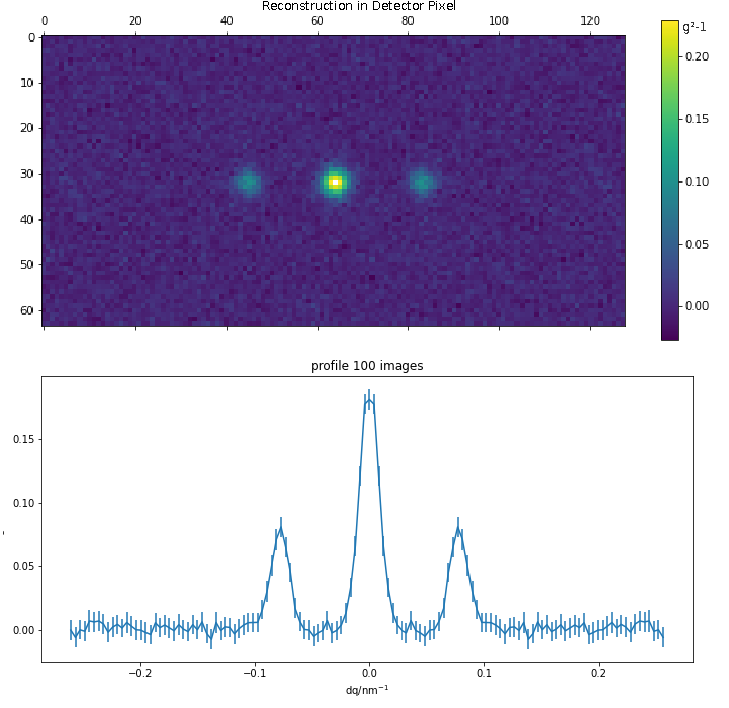
\includegraphics[width=\linewidth]{images/lv65simA.pdf}
		\caption{Nano-Grating}
		\label{fig:outlook_grating}
	\end{subfigure}
	\begin{subfigure}[b]{0.37\textwidth}
		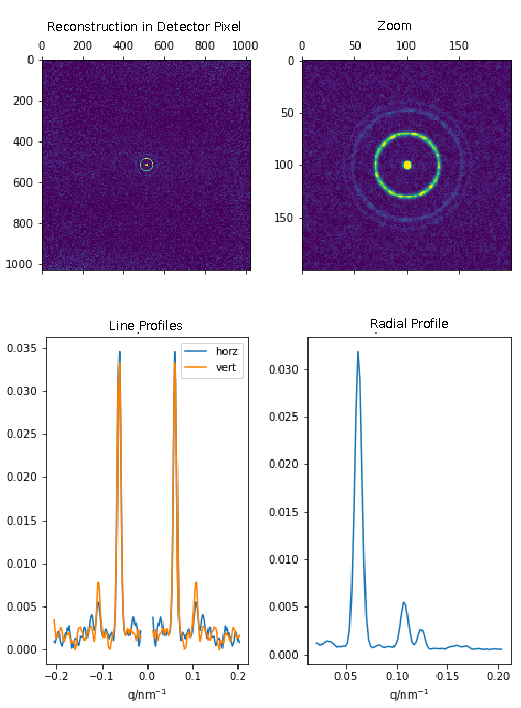
\includegraphics[width=\linewidth]{images/lv65simB.pdf}
		\caption{AAO membrane  }
		\label{fig:outlook_aao}
	\end{subfigure}
	\caption[Simulations in Preparation of LV65 Experiment]{Examples of simulations performed with the tools developed in this thesis in preparation of the LCLS free electron laser experiment LV65, which will use nano-gratings and AAO membranes with metal filled self-organized pores as samples for an IDI measurement. The simulations were used to chose an optimized sample geometry and to estimate the feasibility with respect to the expected SNR. The images shown are the calculated fluorescence intensity correlations between pixels of a quarter of an Jungfrau 4M detector placed at a distance of 70\,cm (grating) and 1\,m (membrane) respectively. The simulated grating has a pitch of 80\,nm, 40\,nm line width and 40\,nm thickness; 20\% excitation and 4 modes were simulated. The AAO membrane has and inter pore distance 105\,nm, the pores are filled with vanadium and 20\% excitation are assumed. For both samples, the average over 100 images is shown.}
\end{figure}

%%%%%%%%%%%%%%%%   ANHANG   %%%%%%%%%%%%%%%%%%



\begin{appendices}
	\addtocontents{toc}{\protect\setcounter{tocdepth}{1}}
	\makeatletter
	\addtocontents{toc}{%
		\begingroup
		\let\protect\l@chapter\protect\l@section
		\let\protect\l@section\protect\l@subsection
	}
	\makeatother
	\chapter{Additional Graphs and Tables}
\section{Simulation}

\begin{table}[h!]
	\caption[Ratio of $g^2-1$ of different photon counting schemes to ground truth value]{Ratio of $g^2-1$ of different photon counting schemes to ground truth value  for $\Delta$=1\, pixel/first maximum. \textit{Closest} is \textit{Combination} without considering Noise photons, giving good results in the low noise cases.}
	\label{tab:photonrecon}

\begin{adjustwidth}{-1em}{-2em}	
\small
\begin{tabular}{lllllll}
	\toprule
	 &        Raw &       Threshold &         Combination &      Closest &         MaxL &          PSANA \\
	\midrule
	Low Signal  &  12 / 0.59 &  6.9 / 0.64 &  0.62 / 0.79 &  0.88 / 0.68 &  0.57 / 0.81 &    -0.5 / 0.66 \\
	High Signal &  2.4 / 1.1 &   1.8 / 1.0 &  0.72 / 0.82 &   1.1 / 0.96 &   1.0 / 0.95 &  -0.026 / 0.79 \\
	High Noise  &  9.3 / 0.3 &  8.1 / 0.39 &   1.0 / 0.58 &   1.3 / 0.46 &  0.44 / 0.54 &   -0.37 / 0.45 \\
	\bottomrule
\end{tabular}
\end{adjustwidth}
\end{table}

\section{Experiment}

\begin{figure}[h!]
	\centering
	\begin{subfigure}[b]{0.45\textwidth}
		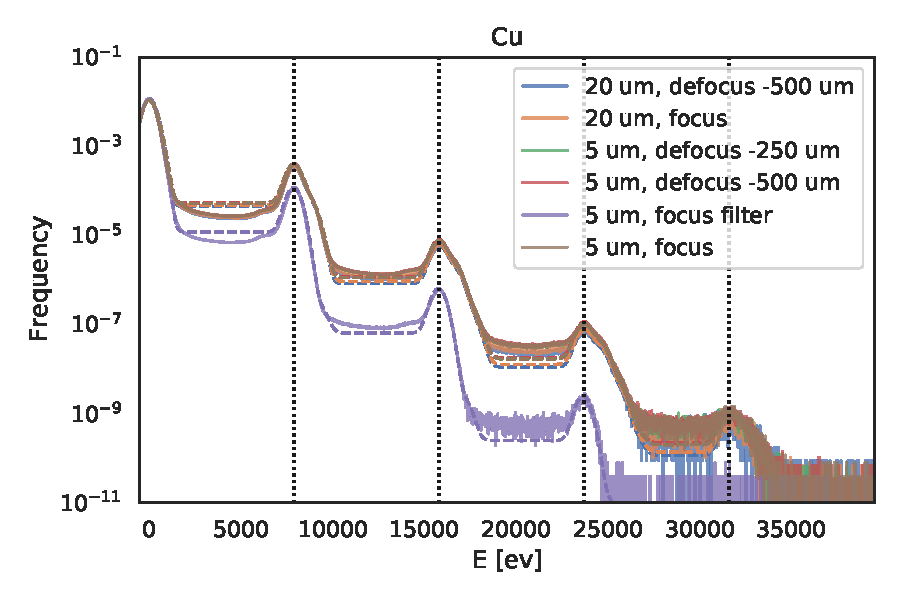
\includegraphics[width=\linewidth]{images/spectrum_foil_cu.pdf}
	\end{subfigure}
	\begin{subfigure}[b]{0.45\textwidth}
		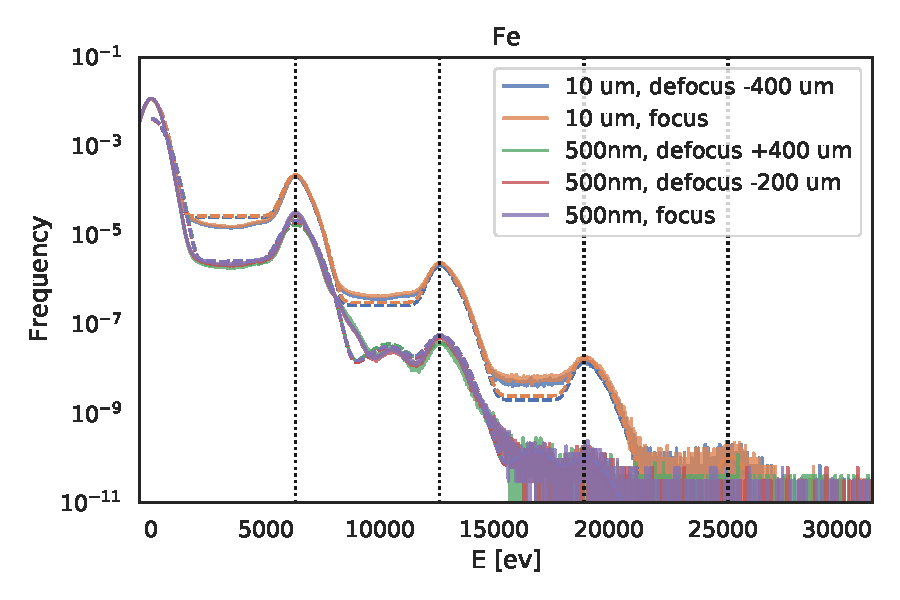
\includegraphics[width=\linewidth]{images/spectrum_foil_fe.pdf}
	\end{subfigure}
	\caption[Spectra of fluorescence using foil samples ]{Spectra of fluorescence using foil samples (left for copper, right for iron) and best fit of the regression using an approximated charge sharing.}
	\label{fig:spectrafoil}
\end{figure}

\begin{figure}[h!]
	\centering
	\begin{subfigure}[b]{0.30\textwidth}
		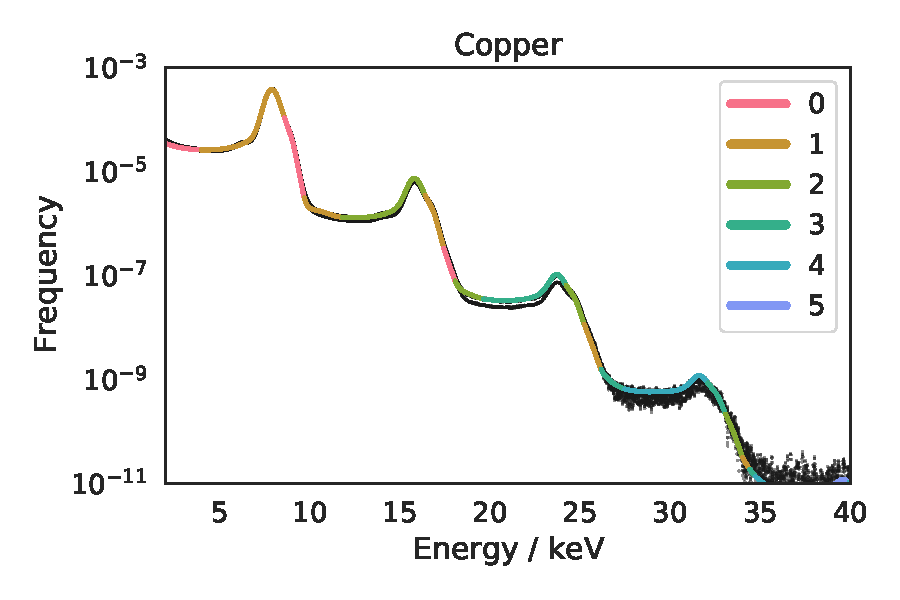
\includegraphics[width=\linewidth]{images/thresholdsCopperHighNoBeta.pdf}
	\end{subfigure}
	\begin{subfigure}[b]{0.30\textwidth}
		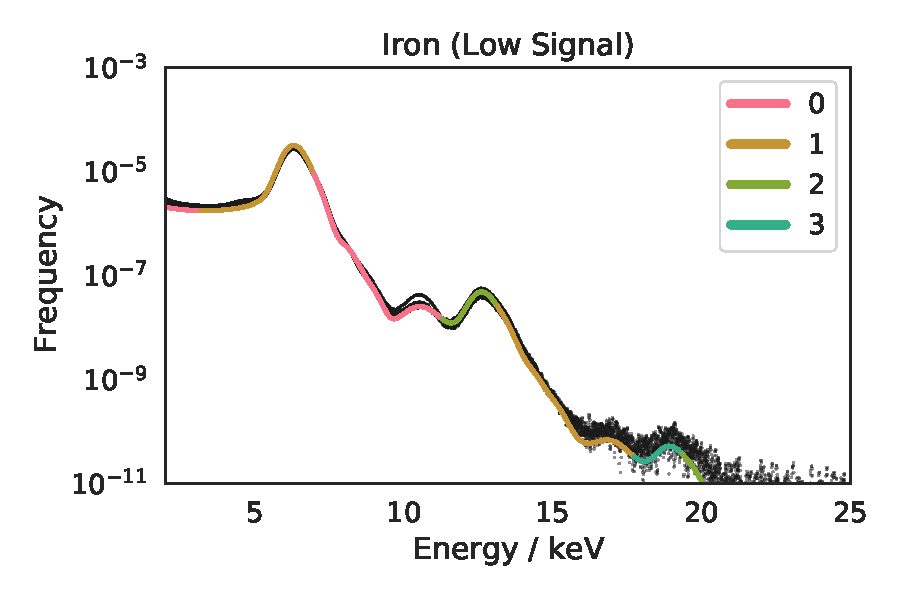
\includegraphics[width=\linewidth]{images/thresholdsIronLow.pdf}
	\end{subfigure}
	\begin{subfigure}[b]{0.30\textwidth}
		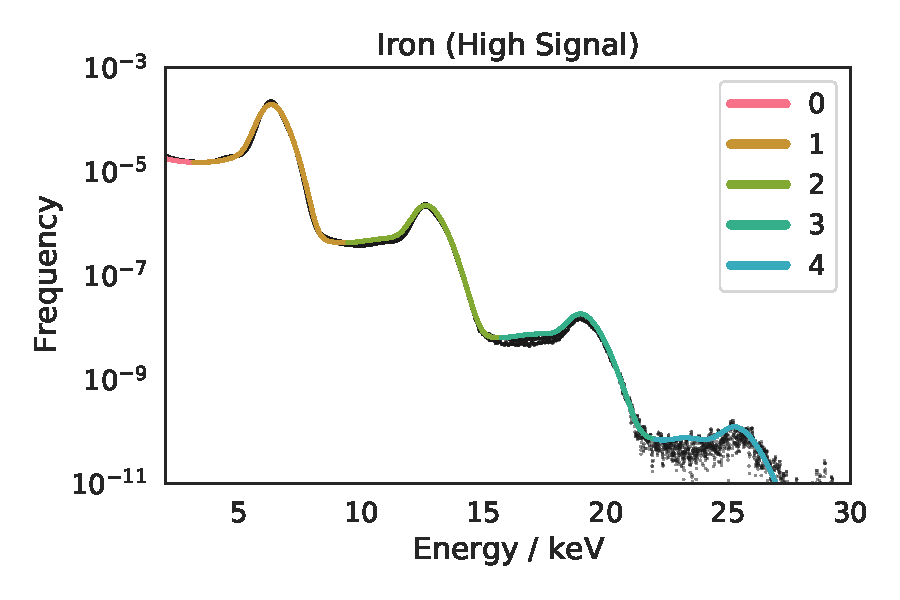
\includegraphics[width=\linewidth]{images/thresholdsIronHigh.pdf}
	\end{subfigure}
	\caption[Spectra of fluorescence using foil samples with photon number classes]{Spectra of fluorescence using foil samples (black), and spectra of the final regression models used for classification, colored by the assigned class of signal photon numbers. The initial values used for the regression are the average values found in the regression using approximated charge sharing, for the sharing width the estimation $\sigma\approx\frac{1}{6} \left(1-\sqrt{1-\rho }\right)$ is used.  The final values of the regression used for classification of photon events are show in \fref{tab:fitvalues}.}
	\label{fig:thresholdsfoil}
\end{figure}
\begin{figure}
	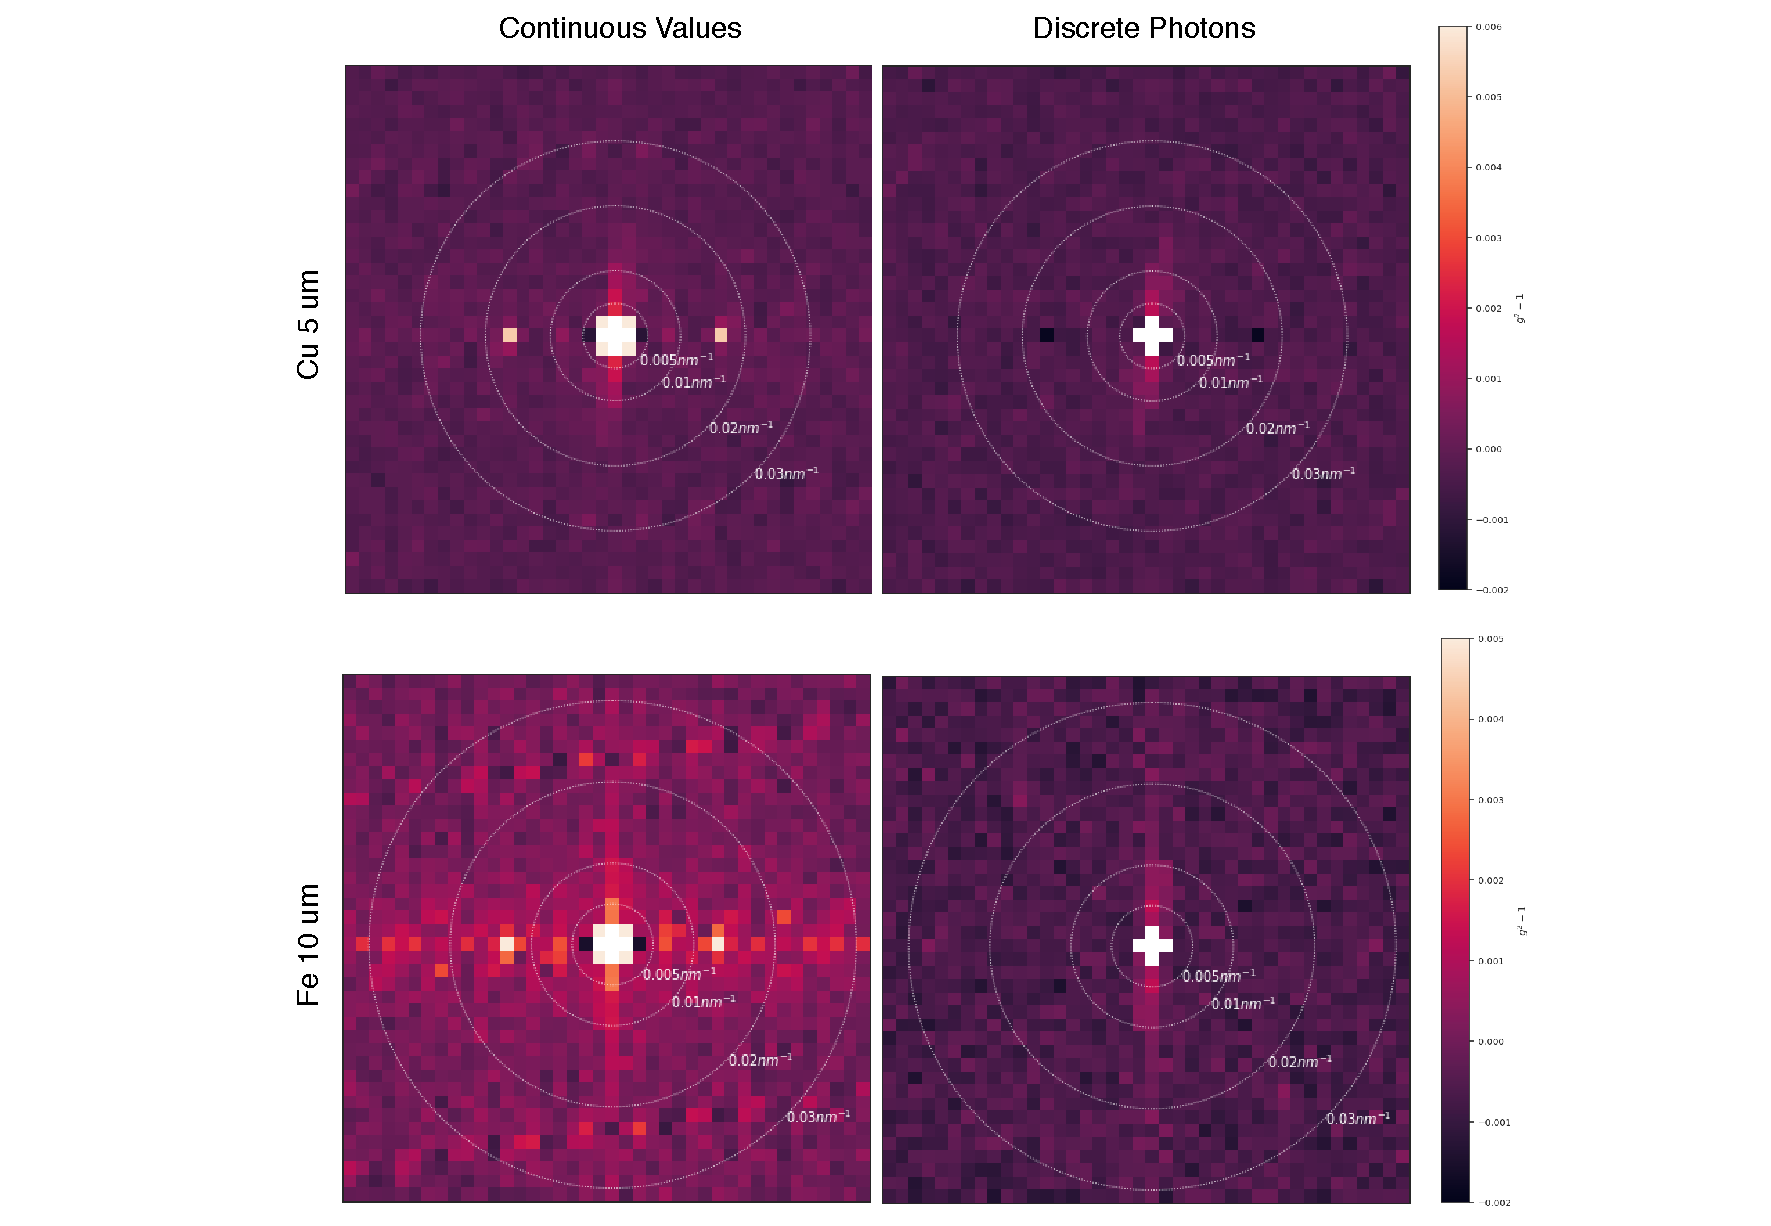
\includegraphics[width=\linewidth]{images/foil_photonmodes.pdf}
	\label{fig:foil_photonmodes}
	\caption[Effect of discretizing the signal into photons]{Effect on the reconstruction of discretizing the signal into photons: For two foils at focal position,  correlations of the continuous, thresholded values read by the detector as well as  correlations after discretizing into photons are shown. Artifacts caused by charge sharing (for example diagonally neighboring pixels being correlated, visible as a square in the center) and other detector imperfections are greatly reduced by discretizing.}
\end{figure}
\begin{table}[h]
	\centering
	\caption[Parameters for simulated spectra used to find thresholds]{Parameters for simulated spectra used to find thresholds. $E_{sig}$/$E_{scat}$ denote the energy of the signal/scattering background photons, $p_{sig}$/$p_{\beta}$/$p_{scat}$ the probability of a signal/K$_{\beta}$/scattering photons, $\sigma_{scat}$ the width (standard deviation) of the (approximated as Gaussian) scattering peak, $\sigma_{det}$ the standard deviation of (assumed as Gaussian) broadening due to detector noise and $\sigma_{sharing}$ the width of the charge sharing cloud.  As the $K_beta$ peak can be distinguished as a shoulder in the Copper spectra, $K_{\beta}$ is considered as noise there and treated like the scattering noise in the classification, resulting in tighter final thresholds ()resulting in partial rejection of  $K_{\beta}$) compared to counting those photons as signal.}
	\label{tab:fitvalues}
		\tiny
	\begin{adjustwidth}{-2em}{-2em}	
\begin{tabular}{lrrrrrrrrrrrr}

	\toprule
	{} &  $E_{sig}$ &  $p_{sig}$ &  $p_{\beta}$ &  $E_{scat}$ &  $p_{scat}$ &  $\sigma_{scat}$ & $E_{scat,2}$ & $p_{scat,2}$ &  $\sigma_{det}$ &   M &  $\sigma_{sharing}$ &  $K_{\beta}$ as noise \\	\midrule
	Copper &          7940 &       4.7e-02 &     1.5e-01 &          10500 &        5.0e-05 &                 450 &           8150 &        5.9e-05 &             350 &  20 &             4.2e-02 &                  True \\
	Iron High         &          6340 &       2.5e-02 &     1.5e-01 &          10700 &        1.5e-05 &                 500 &                &                &             420 &  20 &             3.5e-02 &                 False \\
	Iron Low          &          6320 &       3.3e-03 &     1.5e-01 &          10570 &        3.0e-06 &                 380 &           8000 &        3.7e-05 &             350 &  20 &             3.0e-02 &                 False \\
	\bottomrule
\end{tabular}
\end{adjustwidth}
\end{table}

\begin{figure}[h!]
	\centering
	\includegraphics[width=0.8\linewidth]{images/kossel_gaas.png}
	\caption[Mean image of fluorescence of GaAs after background subtraction with visible Kossel lines ]{Mean images of 5000 shots after background subtraction for sample 1 (left) and sample 2 (right), showing the Kossel lines and some artifacts at the edges.}
	\label{fig:kosselgaasmean}
\end{figure}


\begin{table}[h!]
	\caption[Miller Indices considered in Kossel line least squares regression of GaAs sample]{Miller Indices considered in Kossel line least squares regression of GaAs sample 1 (left) and sample 2 (right). Not all possible Kossel lines are visible in the recorded images.}
	\begin{tabular}[t]{lll}
		\toprule
		h&           k &        l \\
		\midrule
	 1 & -1 &  1 \\
	-1 &  1 &  1 \\
	-1 & -1 &  1 \\
	2 & -2 &  0 \\
	-2 &  2 &  0 \\
	-2 & -2 &  0 \\
	2 &  2 &  0 \\
	-3 & -1 &  1 \\
	3 &  1 &  1 \\
	-1 & -3 &  1 \\
	2 & -2 &  4 \\
	-2 & -2 &  4 \\
	2 &  2 &  4 \\
	-2 &  2 &  4 \\
	-4 &  0 &  4 \\
	0 &  4 &  4 \\
	4 &  0 &  4 \\
	0 & -4 &  4 \\
				\bottomrule
	\end{tabular}
\hspace{1cm}
	\begin{tabular}[t]{lll}	
	\toprule
	h&           k &        l \\
	\midrule
 2 &  2 &  0 \\
-2 &  2 &  0 \\
2 & -2 &  0 \\
0 & -2 &  2 \\
0 &  2 &  2 \\
2 &  0 &  2 \\
-2 & -2 &  0 \\
-2 &  0 &  2 \\
-3 & -1 &  3 \\
-1 & -3 &  3 \\
1 &  3 &  3 \\
3 &  1 &  3 \\
-1 &  3 &  3 \\
1 & -3 &  3 \\
0 & -4 &  4 \\
-4 &  0 &  4 \\
0 &  4 &  4 \\
4 &  0 &  4 \\
0 &  2 &  6 \\
2 &  0 &  6 \\
-2 &  0 &  6 \\
0 & -2 &  6 \\
	\bottomrule
\end{tabular}
\end{table}
\FloatBarrier

	\chapter{Implementation Details}
All source code is made available under \url{https;//github.com/fzimmermann89/msc}.
In \fref{algo:td} the procedure for time dependent simulations is show in detail.
\begin{algorithm}
	\caption{Time dependent Simulation}\label{timesim}
	\begin{algorithmic}
		\Procedure{Scan}{$x \in \mathbb{C}^N$, $t \in \mathbb{R}^N$, $\tau\ \in \mathbb{R}$}
		\Comment{Exponentially decaying inclusive prefix sum} 
		\State $s \gets 1$
		\While{$s<N$} 
		\Comment{Scan Upsweep}
		\For{k  $\gets 0$ to $N-1$ step $2s$ \textbf{parallel}}
		\State $decay \gets exp\left(\frac{t[k+s-1]-t[k+2s-1]}{\tau}\right)$ 
		\State $x[k+2s-1] \gets x[k+2s-1] + decay*x[k+s-1]$				
		\EndFor
		\State $s \gets 2s$ 
		\EndWhile
		\State $s \gets N/2$
		\While{$s>1$}  
		\Comment{Scan Downsweep}
		\State $s \gets s/2$
		\For{k  $\gets 0$ to $N-1-2s$ step $2s$ \textbf{parallel}}
		\State $decay \gets exp\left(\frac{t[k+2s-1]-t[k+3s-1]}{\tau}\right)$
		\State $x[k+3s-1] \gets x[k+3s-1] + decay*x[k+2s-1]$
		\EndFor
		\EndWhile
		\EndProcedure
		\Function {Prepare}{$x \in \mathbb{R}^{Nx3}$,  $y \in \mathbb{R}^{3}$, $t_0 \in \mathbb{R}^N$, $\phi \in [0,2\pi)^N$}
		\Comment{ommitted for brevity}
		\State \Return Time independent fields $a \in \mathbb{C}^N$, Arrival times $t \in \mathbb{R}^N$ for each atom
		\EndFunction
		\Function{Simulation}{Atom positions $x \in \mathbb{R}^{Nx3}$,  Detector position $y \in \mathbb{R}^{3}$, \newline Initial Phases $\phi \in [0,2\pi)^N$, Emission Times $t_0 \in \mathbb{R}^N$, $\tau\ \in \mathbb{R}$}
		\State	(a, t) = \Call {Prepare}{$x$, $y$, $\phi$}
		\State	\Call{Sort}{} ($a$,$t$) by $t$
		\State 	\Call{Scan}{$a$, $t$, $\tau$}
		\State $Result \gets \frac{\tau}{2} \left|a_N\right|^2 -\frac{\tau}{2}\sum_{n=1}^{N-1} \left|a_n\right|^2 \left(exp(-2 (t_{n+1}-t_n)/\tau)-1\right)$   
		\State \Return $Result$
		\EndFunction
		
	\end{algorithmic}
	\label{algo:td}
\end{algorithm}
\clearpage

The algorithm used to sample points a minimum distance apart from inside an n-dimensional volume used in the simulation of multiple samples inside the focal volume based on an algorithm first described by Bridson is shown in \fref{algo:bridson} \cite{bridson}. To draw random points uniformly from the annulus between $d$ and $2d$ around an existing point, the radius is sampled from the inverse of the radial CDF and the direction is generated using normalized n-dimensional normal distributed coordinates \cite{muller1959}.
An example of generated points is shown in \fref{fig:bridson}.
\begin{algorithm}
	\caption{Bridson's Poisson Sampling Algorithm}\label{algo:bridson}
	\begin{algorithmic}
		\Function{bridson}{ndim,d,r}
			\State $cellsize \gets d / \sqrt(ndim)$
			\State $grid \in \mathbb{Z}^{{{(2(r+d)/cellsize)}^{ndim}}} \gets 0$
			\State $Initialpoint \sim (2\mathcal{U}^2-1)*r$
			\State $queue \gets$ List(1)
			\State $points \gets$ List(Initialpoint)
			\While{queue}
				\State $ActivePoint \gets$ \textbf{pop} \textit{random element from queue}
				\Loop{k times}:
					\State $Candidate \gets$\Call{DrawCandidate}{$ActivePoint$}
					\If{\Call{Fits}{$Candidate$}}
						\State \textit{mark in grid}
						\State \textbf{add} $Candidate$ to $points$
						\State \textbf{add} $Candidate$ to $queue$
					\EndIf
				\EndLoop
			\EndWhile
			\State \Return $points$
		\EndFunction
		
		\Function {PointFits} {point, points, grid,d}:
			\State find points coordinate in grid
			\ForAll{cells less than d+cellsize away}
				\If{$cell\neq 0$}
					\State neighbor$\gets$ points[cell]
					 \If{$\left|neighbor-points\right|_2<d$} 	
					 	\State \Return False 
					 \EndIf
				\EndIf
			\EndFor
			\State \Return True
		\EndFunction
		\Function{DrawCandidate}{AroundPoint}
			\State $u \sim \mathcal{U}$
			\State $r \gets d * (1 + (2 ^ {ndim} - 1) * u) ^ {\sfrac{1}{ndim}}$
			\State $n \sim \mathcal{N}^{ndim}$
			\State \Return  $n/|n|_2 * r + AroundPoint$
		\EndFunction
	\end{algorithmic}
\end{algorithm}

\begin{figure}[H]
	\centering
	\includegraphics[width=0.4\linewidth]{images/bridson.pdf}
	\caption[Points generated by the Bridson algorithm inside a 2D circle]{Points generated by the Bridson algorithm inside a 2D circle (r=50) with a minimum distance of d=2.}
	\label{fig:bridson}
\end{figure}



%\cite{born1980,griffiths2005}
%\cite{mandel1995,baym1997,zernike1938,santra2009,sorum1987,lajunen04,tono2013}


	\addtocontents{toc}{\endgroup}
\end{appendices}


%%%%%%%%%   LITERATURVERZEICHNIS   %%%%%%%%%%%

%\nocite{*}
\singlespacing
\bibliography{ffz}
\bibliographystyle{ffz}
\addcontentsline{toc}{chapter}{Bibliography}
\cleardoublepage




\end{document}
